\section{はじめに}
OOD検知は，学習時のクラス（ID）以外の入力を見分ける問題である．CLIP~\cite{radford2021clip}などのVLMは学習なしにOODを検知でき~\cite{ming2022mcm}，負例ラベル~\cite{jiang2024neglabel}やテスト時の適応~\cite{zhang2024adaneg,zhang2026tanl,xu2026interneg,yang2026tins}でfar-OODの\AUC{}は97\%に達したが，IDに近いnear-OODは難しい．OpenOOD v1.5~\cite{zhang2023openood}のImageNet-1Kでは，VLMによる最良の報告値でもnear-OODの\AUC{}は82.65\%，\FPR{}は57.88\%にとどまり~\cite{yang2026tins}，ImageNet-1Kのラベルで学習した検出器~\cite{park2023nnguide,li2024moodv2}や教師なし生成モデルのDisCoPatch~\cite{caetano2025discopatch}でも\FPR{}は29--48\%残る（\tabref{main}）．

本研究は，凍結した特徴抽出器とIDクラスあたり16枚のラベル付き画像だけで，この残りを学習なしで減らす転導的な枠組み\textbf{Salmon Ladder}を提案する．支持画像・ラベル付きの参照画像と較正画像・テスト画像を節点とする1つのグラフの上で，支持画像に置いた質量を伝播させ，届いた質量をラベル付き画像の中での順位（\textbf{較正順位}）で読む．支持画像から遠く互いに近い未知の塊には質量が届かず，較正順位はAdaDetect~\cite{marandon2024adadetect}の意味での共形$p$値になる．この伝播だけで見出しの数字の大半が得られる（\tabref{abl}）．その上で，テスト集合に同じ未知クラスの画像が複数枚含まれる（\textbf{再出現}）ときの拡張として，偽発見率を制御する多重検定で未知の側に偏った画像を自己ラベル付けして\textbf{種}にし，種に置いた質量を同じグラフで伝播させて同じクラスの残りの未知を引き上げる\footnote{コード：\url{https://github.com/omotes24/SalmonLadder}}．種の選択と読み出しの順位を参照画像に対して取ることで，テスト画像を折に分けずに，種を含む読み出しの較正順位そのものが共形$p$値になる．

主たる設定はテスト集合全体を見て採点する\textbf{事後採点}（transductive）で，\textbf{到着時採点}も示す（付録\ref{sec:app_online}）．貢献は4点である．(1) \textbf{共形ラベル伝播}：グラフ上のラベル伝播を共形$p$値として読む検知器（命題1--3）．学習なし・16枚のラベルだけで，OpenOOD v1.5 ImageNet-1Kのnear-OODで\AUC{} \NRAloneNearAuroc\%，\FPR{} \NRAloneNearFpr\%（6通りの抽出の平均，単体）を達成し，公開の最良値を\AUC{}で\NRAloneGapNearAuroc{}ポイント，\FPR{}で\NRAloneGapNearFpr{}ポイント更新した（\tabref{main}）．far-OODとFour-OOD~\cite{huang2021mos}でも最良で，構成を固定したまま評価したImageNet-200とCIFAR-100でも報告値の最良を上回る（\secref{in200}）．$u^{+}=\sqrt{\delta}\times$（確率）の分解で，確率の因子が検知の大半を担い，密度の因子は単独では手がかりにならず確率の因子と組んで効く（向きはデータセットに依る）ことを示す（\secref{abl}）．(2) \textbf{種と参照画像}：種は再出現（クラスあたり10枚以上）のときの拡張で，ImageNet-1Kのnear-OODで\FPR{}を\NRvsLpAloneNearDAbs{}（単体）／\NRvsLpTinsNearDAbs{}（$\times$TINS）ポイント下げるが，未知が大半を占めるImageNet-200とCIFAR-100では効かない．参照画像による読み出し$\sR$は折なしで共形$p$値になり（命題4），較正画像とテスト画像が交換可能なら，利用者は閾値を「IDの誤警報率$\alpha$」として直接指定できる．同じ未知クラスの画像に小さな$p$値を保証する分離の上界（系2）を導き，格子で実測する（\secref{rec}）．(3) \textbf{比較と限界}：同じ特徴の静的な検出器，同じグラフ上のクラスラベル伝播，全学習画像を使う基線，ゼロショットの手法と比べて利得の出どころを切り分け（\tabref{abl}，\secref{in200}），1枚だけ現れる未知には静的な検出器より弱く，描画への共変量シフト（ImageNet-R）をIDとして受け入れないことを示す（\secref{rec}，\secref{csid}）．(4) \textbf{選択手続きと逸脱の開示}：構成は開発用分割の事前登録した規則で選び，登録からの逸脱2件（いずれもテスト集合の値を見た後）と，開発用分割が構成の細部（$q$や種の規則）の差を予測しないことを開示する（\secref{exp}）．

\begin{figure}[t]
\centering
\scalebox{0.76}{% 図1：Salmon Ladder の概要（1段幅 8.4 cm 以内）．(a) 1つのグラフと支持画像からの質量 u+，(b) 参照画像での順位 p+ への BH 法で種を選ぶ（プール全体，折なし），(c) 種からの質量 u- と参照画像による読み出し sigma_ref, p_fin．
\providecommand{\figfont}{\fontsize{6.74pt}{8pt}\selectfont}
\begin{tikzpicture}[font=\figfont, >={Latex[length=1.3mm]}, x=1cm, y=1cm,
  sup/.style={draw=black, fill=black!75, minimum size=0.21cm, inner sep=0pt},
  idsq/.style={draw=black!55, fill=black!10, minimum size=0.19cm, inner sep=0pt},
  oodA/.style={draw=blue!60!black, fill=blue!35, minimum size=0.22cm, inner sep=0pt, regular polygon, regular polygon sides=3},
  seed/.style={draw=red!70!black, fill=red!45, minimum size=0.22cm, inner sep=0pt, regular polygon, regular polygon sides=3},
  calp/.style={draw=blue!70!black, fill=white, line width=0.6pt, minimum size=0.17cm, inner sep=0pt, circle},
  refp/.style={draw=teal!70!black, fill=teal!30, line width=0.5pt, minimum size=0.2cm, inner sep=0pt, diamond},
  edge/.style={black!45, line width=0.45pt},
  flow/.style={->, orange!85!black, line width=0.7pt},
  nflow/.style={->, red!70!black, line width=0.7pt},
  box/.style={draw, rounded corners=2pt, align=center, inner sep=2pt},
  lab/.style={inner sep=1pt, font=\figfont}]
% ================================================================ (a) one graph, mass from the support
\node[lab, anchor=west, font=\figfont\bfseries] at (0,6.6) {(a) 1つのグラフ：支持画像の質量 $u^{+}$ が辺を伝わる};
\node[sup] (s1) at (0.55,5.8) {}; \node[sup] (s2) at (1.05,6.05) {}; \node[sup] (s3) at (1.45,5.65) {};
\node[calp] (c1) at (0.9,5.35) {}; \node[refp] (c2) at (1.9,5.2) {};
\node[idsq] (t1) at (0.4,5.1) {}; \node[idsq] (t2) at (1.35,4.95) {}; \node[idsq] (t3) at (2.2,5.8) {}; \node[idsq] (t4) at (2.6,4.9) {};
\node[oodA] (q1) at (3.4,5.2) {}; \node[oodA] (q2) at (3.95,5.5) {}; \node[oodA] (q3) at (3.8,4.8) {}; \node[oodA] (q4) at (4.4,5.05) {};
\foreach \a/\b in {s1/s2, s2/s3, s1/t1, s1/c1, s2/c1, s3/t2, s3/c2, s3/t3, c1/t1, c1/t2, t2/c2, t3/c2, t2/t4, c2/t4, t4/q1, q1/q2, q1/q3, q2/q3, q2/q4, q3/q4, q1/q4}{\draw[edge] (\a) -- (\b);}
\draw[flow] (s1) to[bend right=12] (t1); \draw[flow] (s3) to[bend left=12] (t3); \draw[flow] (s3) to[bend right=10] (t2);
\draw[flow, orange!60!black, line width=0.5pt] (t2) to[bend right=8] (t4);
\draw[flow, orange!50!black, line width=0.35pt, densely dashed] (t4) -- (q1);
\node[lab, anchor=north west, align=left] at (4.6,6.2) {ID：支持画像に近く $u^{+}$ 大\\未知：互いに近く支持画像\\\quad から遠く $u^{+}$ 小\\参照 $\mathcal{R}$・較正 $\mathcal{C}$ も同じ節点};
\node[lab, anchor=west] at (0.0,4.5) {\tikz{\node[sup]{};}\,支持 $\mathcal{S}$\ \tikz{\node[refp]{};}\,参照 $\mathcal{R}$\ \tikz{\node[calp]{};}\,較正 $\mathcal{C}$\ \tikz{\node[idsq]{};}\,テスト（ID）\ \tikz{\node[oodA]{};}\,未知\ \tikz{\node[seed]{};}\,種};
% ================================================================ (b) BH selection on the calibrated ranks
\node[lab, anchor=west, font=\figfont\bfseries] at (0,4.0) {(b) $p^{+}$（参照画像 $\mathcal{R}$ の中での $u^{+}$ の順位）に BH 法をかけて種を選ぶ};
\draw[->, black!45] (0.3,3.2) -- (8.1,3.2);
\node[lab, anchor=north west, black!65] at (0.3,3.15) {$p^{+}$ 小（未知らしい）};
\node[lab, anchor=north east, black!65] at (8.1,3.15) {$p^{+}$ 大（ID らしい）};
\foreach \x in {0.5,0.62,0.72,0.84,0.98,1.1,1.26,1.45} {\node[seed] at (\x,3.42) {};}
\foreach \x in {1.95,2.4,3.1} {\node[oodA] at (\x,3.42) {};}
\foreach \x in {1.7,2.2,2.7,3.4,3.75,4.1,4.5,4.9,5.3,5.7,6.1,6.5,6.9,7.3,7.7} {\node[idsq] at (\x,3.41) {};}
\draw[red!70!black, line width=0.8pt, densely dashed] (1.58,3.72) -- (1.58,3.15);
\node[lab, red!70!black, anchor=west] at (1.65,3.75) {種 $\hat{Q}$：$p_{(i)}\le q\,i/(\hat{\pi}_0 m)$ を満たす最大の $i$ まで};
\node[lab, anchor=west] at (0.3,2.6) {AdaDetect の BH 法（$q{=}0.2$）：交換可能なら偽発見率 $\le q$（命題3）};
\node[lab, anchor=west] at (0.3,2.36) {枚数 $\hat{k}$ は固定しない．候補は較正画像とテスト画像のすべて（折なし）};
% ================================================================ (c) mass from the seeds and the read-out
\node[lab, anchor=west, font=\figfont\bfseries] at (0,1.6) {(c) 種の質量 $u^{-}$ を同じグラフで伝播させ，参照画像で読む};
\node[sup] (b1) at (0.55,0.85) {}; \node[sup] (b2) at (1.05,1.1) {};
\node[calp] (d1) at (0.9,0.4) {}; \node[idsq] (e1) at (0.4,0.15) {}; \node[idsq] (e2) at (1.35,0) {}; \node[idsq] (e3) at (2.2,0.85) {}; \node[idsq] (e4) at (2.6,-0.05) {};
\node[seed] (f1) at (3.4,0.25) {}; \node[seed] (f2) at (3.95,0.55) {}; \node[oodA] (f3) at (3.8,-0.15) {}; \node[oodA] (f4) at (4.4,0.1) {};
\foreach \a/\b in {b1/b2, b1/e1, b1/d1, b2/d1, b2/e3, d1/e1, d1/e2, e2/e4, e3/e4, e4/f1, f1/f2, f1/f3, f2/f3, f2/f4, f3/f4, f1/f4}{\draw[edge] (\a) -- (\b);}
\draw[nflow] (f1) to[bend right=12] (f3); \draw[nflow] (f2) to[bend left=12] (f4);
\draw[nflow, red!50!black, line width=0.35pt, densely dashed] (f1) -- (e4);
\node[lab, anchor=north west, align=left] at (4.6,1.25) {種に近い未知：$u^{-}$ 大\\\quad $\Rightarrow p^{-}$ 小\\ID：種から遠く $u^{-}$ 小\\\quad $\Rightarrow p^{-}$ 大\\種が同じクラスの\\\quad 残りを引き上げる};
\node[box, fill=yellow!15, anchor=west, align=left] (ro) at (0.3,-1.0) {$\sigma_{\mathrm{ref}}(x)=\sum_{v}\log p^{+}_{v}(x)\,p^{-}_{v}(x)$\\$s(x)=s_0(x)\exp\sigma_{\mathrm{ref}}(x)$};
\node[lab, anchor=west, align=left] at (4.3,-1.0) {$p^{\pm}$：参照画像 $\mathcal{R}$ での順位\\$p^{\mathrm{fin}}$：$\sigma_{\mathrm{ref}}$ の較正画像 $\mathcal{C}$ での順位（命題4）\\$s_0$：ベース検出器（TINS），$v$：ビュー};
\end{tikzpicture}
}
\caption{Salmon Ladderの概要．(a) 支持画像$\mathcal{S}$・参照画像$\mathcal{R}$・較正画像$\mathcal{C}$・テスト画像$\mathcal{T}$を節点とする1つの$k_g$近傍グラフで，支持画像に置いた質量$u^{+}$を伝播させる．(b) $u^{+}$を$\mathcal{R}$の中での順位$p^{+}$（共形$p$値）に変え，偽発見率を制御するBH法で棄却された画像を種$\hat{Q}$とする（候補は$\mathcal{C}\cup\mathcal{T}$）．(c) 種に置いた質量$u^{-}$を同じグラフで伝播させ，$\mathcal{R}$の中での逆順位に変えて足した統計量$\sR$を，$\mathcal{C}$の中での順位$\pfin$で読む．スコアは$s_0\exp\sR$（$s_0$はベース検出器）．}
\label{fig:overview}
\end{figure}

\section{提案手法}
\label{sec:method}
\subsection{問題設定と全体像}
IDの各クラス$c$に16枚のラベル付き画像が与えられ，12枚を支持画像$\mathcal{S}_c$，2枚を参照画像$\mathcal{R}_c$，2枚を較正画像$\mathcal{C}_c$とする（クラスごとの並びの位置で固定；全体を$\mathcal{S}$，$\mathcal{R}$，$\mathcal{C}$，$|\mathcal{R}|=|\mathcal{C}|=2{,}000$）．テスト集合$\mathcal{T}$はIDとOODが混ざったラベルなしの画像の集合で，各画像$x\in\mathcal{T}$にスコア$s(x)$（大きいほどIDらしい）を返す．主たる設定は$\mathcal{T}$の全画像が揃ってから採点する\textbf{事後採点}（transductive）で，画像が届くたびに採点する\textbf{到着時採点}は付録\ref{sec:app_online}で扱う．特徴抽出器$f$は凍結し，モデルは更新しない．Salmon Ladderは次の4つの部品からなる（\figref{overview}）．
\begin{enumerate}
\setlength{\itemsep}{0pt}
\item \textbf{較正順位}：IDらしさの値を，固定したラベル付き画像の中での順位に変えて読む（\secref{rank}）．すべての部品の共通の物差しで，共形$p$値である．
\item \textbf{支持画像からの質量$u^{+}$}：支持画像・参照画像・較正画像・テスト画像を節点とする1つのグラフ上で支持画像に置いた質量を伝播させ，参照画像の中での順位$\pP$で読む（\secref{graph}）．
\item \textbf{未知からの質量$u^{-}$}：$\pP$に偽発見率を制御する多重検定（AdaDetect~\cite{marandon2024adadetect}の意味でのBH法）をかけ，較正画像とテスト画像の全体から未知の側に偏った画像の集合$\hat{Q}$（種）を自己ラベル付けし，種の質量を同じグラフで伝播させる（\secref{seed}）．
\item \textbf{参照画像による読み出し}：2つの質量の参照画像での順位を足した統計量$\sR$を，較正画像の中での順位$\pfin$で読む（\secref{ref}）．$\pfin$は折に分けずに共形$p$値になり，IDの誤警報率とBH法の偽発見率が保証される（命題4）．
\end{enumerate}
スコアは$s(x)=s_0(x)\exp\sR(x)$で，$s_0$は任意のベース検出器である（\secref{score}）．判定には$\pfin$を使う．

\subsection{較正順位：固定したラベル付き画像の中での順位}
\label{sec:rank}
IDらしさを表す値$a(x)$（小さいほどOODらしい）を，ラベル付き画像の集合$\mathcal{C}'$（$n'=|\mathcal{C}'|$）を同じ方法で採点した値の中での順位
\begin{equation}
p(x)=\frac{1+|\{x'\in\mathcal{C}':a(x')\le a(x)\}|}{n'+1}\in\Big[\frac{1}{n'+1},1\Big]
\label{eq:rank}
\end{equation}
で読む（\textbf{較正順位}）．$\mathcal{C}'$とIDのテスト画像が交換可能で，$a$が両者を対称に扱うなら，これは$\Pr(p(x)\le\alpha)\le\alpha$を満たす共形$p$値~\cite{bates2023conformal,marandon2024adadetect}であり，閾値$\alpha$でOODと判定したときのIDの誤警報率は$\alpha$以下になる．大きいほどOODらしい値は不等号を逆にして読む（\eqnref{pneg}）．順位は$[0,1]$の値なので尺度の違うビューどうしの積が取れる．

\subsection{支持画像からの質量：ラベル伝播のグラフ}
\label{sec:graph}
\subsubsection{グラフの構成}
支持画像$\mathcal{S}$，参照画像$\mathcal{R}$，較正画像$\mathcal{C}$，テスト画像$\mathcal{T}$のすべてを節点とする（節点数$N$）．各節点$i$から，コサイン類似度$f(x_i)^{\top}f(x_j)$が上位$k_g{=}10$の節点$j$へ向かう辺を張り，重みを$a_{ij}=\max(f(x_i)^{\top}f(x_j),0)$とする（行列$A$）．向きのない辺にするために$W=\max(A,A^{\top})$（成分ごとの最大）とし，次数$\delta_i=\sum_jW_{ij}$，$D=\mathrm{diag}(\delta_i)$，正規化した行列
\begin{equation}
S=D^{-1/2}WD^{-1/2}
\label{eq:S}
\end{equation}
を作る~\cite{zhou2004lgc}．$S$は対称で固有値は$[-1,1]$にあり，非零成分は$O(Nk_g)$の疎行列である．参照画像・較正画像・テスト画像はどれもラベルを持たない節点として全く同じ扱いを受け，グラフは節点の順序や名札に依らない（付録の\figref{graph}a）．グラフはビューごとに1つ作り，2つの質量を同じグラフで伝播させる．

\subsubsection{伝播の反復とランダムウォークとしての意味}
支持画像の節点で1，他で0のベクトル$\mathbf{y}^{+}\in\{0,1\}^{N}$と$\lambda{=}0.9$で
\begin{equation}
\mathbf{u}^{(\ell+1)}=\lambda S\mathbf{u}^{(\ell)}+(1-\lambda)\mathbf{y}^{+}
\label{eq:lp}
\end{equation}
を収束するまで反復する（$\mathbf{u}^{(0)}=\mathbf{0}$；局所・大域一貫性~\cite{zhou2004lgc}の反復）．$\lambda<1$かつ$\|S\|_2\le1$なので縮小写像であり，収束解$\mathbf{u}^{+}=(1-\lambda)\sum_{\ell\ge0}\lambda^{\ell}S^{\ell}\mathbf{y}^{+}$を持つ．ランダムウォークで言えば，$P=D^{-1}W$を遷移確率とし，各ステップで確率$1-\lambda$で止まるランダムウォークを節点$i$から始めたとき，
\begin{equation}
u^{+}_i=\sqrt{\delta_i}\;q_i,\qquad q_i=\mathbb{E}_i\Big[\frac{\mathbf{1}[X_T\in\mathcal{S}]}{\sqrt{\delta_{X_T}}}\Big]
\label{eq:walk}
\end{equation}
である（$X_T$は止まった節点．$S^{\ell}=D^{1/2}P^{\ell}D^{-1/2}$から従う）．$u^{+}$は，次数（密度）の因子$\sqrt{\delta_i}$と，支持画像で止まる確率（止まった支持画像の$1/\sqrt{\delta}$で重みづけたもの）の因子$q_i$の積である．支持画像に近いID画像からは数歩で支持画像に着くので$q$は大きく，互いに近い未知の塊からは支持画像へ出る辺が少ないので$q$は小さい（\figref{graph}a；どちらの因子がnearとfarに効くかは\secref{abl}）．

\subsubsection{参照画像での順位による読み出し}
参照画像はグラフの節点であり（$y^{+}=0$），同じ反復で$u^{+}$を受け取るので，
\begin{equation}
\pP(x)=\frac{1+|\{r\in\mathcal{R}:u^{+}(r)\le u^{+}(x)\}|}{|\mathcal{R}|+1}
\label{eq:plp}
\end{equation}
とする．$u^{+}$は支持画像の特徴と「参照画像・較正画像・テスト画像を合わせた集合」だけで決まり，その集合の中の節点を入れ替えても各画像の値は変わらない（置換不変性）．したがって参照画像とIDのテスト画像が交換可能なら，$\pP$はAdaDetect~\cite{marandon2024adadetect}の経験$p$値で，IDのテスト画像について超一様である．$\pP$だけでも検知器として完結し（\tabref{abl}の「$\pP$のみ」），以下の種は再出現する未知のための拡張である．

\subsubsection{質量の保存とカットの上界}
\label{sec:mass}
\textbf{命題1（質量の保存）．}$\bom=D^{1/2}\mathbf{1}$とすると，\eqnref{lp}を$\mathbf{u}^{(0)}=\mathbf{0}$から$L$回反復した値は$\bom^{\top}\mathbf{u}^{(L)}=(1-\lambda^{L})\sum_{j\in\mathcal{S}}\sqrt{\delta_j}$を満たし，収束解では$\bom^{\top}\mathbf{u}^{+}=\sum_{j\in\mathcal{S}}\sqrt{\delta_j}$である（証明は付録\ref{sec:app_proofs}）．重みづけた質量の総和は支持画像の次数だけで決まり，テスト画像の枚数に比例しては増えないので，1節点あたりの$u^{+}$の尺度はテスト集合やビューごとに変わり（\figref{graph}c），値をそのまま閾値にかけたりビューどうしで掛けたりはできない．順位\eqnref{plp}がこの尺度を取り除く．
\label{sec:cut}
\textbf{命題2（カットの上界）．}初期質量を置いた節点の集合$Y$を含まない節点の集合$Q$について，$Q$と外とを結ぶ辺の重みの和を$w(Q,\bar{Q})=\sum_{i\in Q,\,j\notin Q}W_{ij}$とすると，収束解$\mathbf{u}$は
\begin{equation}
\sum_{i\in Q}\sqrt{\delta_i}\,u_i\le\frac{\lambda}{1-\lambda}\cdot\frac{w(Q,\bar{Q})}{\min_{j\in Y}\sqrt{\delta_j}}
\label{eq:cond}
\end{equation}
を満たす（証明は付録\ref{sec:app_proofs}）．$W=\max(A,A^{\top})$なので，$w(Q,\bar{Q})$には\textbf{$Q$の節点が自ら張る辺}と\textbf{外の節点が$Q$へ張る辺}の両方が入る（\figref{graph}b）．$Y=\mathcal{S}$，$Q$を同じ未知クラスの$r$枚とし，それらが互いの近傍の上位を占めるなら，前者は節点あたり$(k_g-r+1)_+$本に減り，$r\ge k_g+1$で尽きる．後者は外の節点が$Q$の画像を近傍に選ぶかどうかで決まる．

\textbf{系1（逃げる確率）．}$Q$の節点$i$から出たランダムウォークが止まる前に$Q$の外へ出る確率を$\pi_i$とすると，$\boldsymbol{\pi}=\lambda(I-\lambda P_{QQ})^{-1}\mathbf{e}$（$P_{QQ}$は$P$の$Q$への制限，$e_i=\sum_{j\notin Q}W_{ij}/\delta_i$）で，$\pi_i\le\psi(\bar e_Q)$，$\bar e_Q=\max_{i\in Q}e_i$，$\psi(e)=\lambda e/(1-\lambda+\lambda e)$である．$\partial Q$を$Q$に隣接する外の節点の集合とすると，$Q$の各節点$i$で
\begin{equation}
u_i\le b_i:=\pi_i\sqrt{\delta_i}\max_{j\in\partial Q}\frac{u_j}{\sqrt{\delta_j}}
\label{eq:esc}
\end{equation}
が成り立つ．特に$\bar e_Q=0$なら$u^{+}_i=0$で，$\pP(i)$は床$1/(|\mathcal{R}|+1)$に落ちる（参照画像の$u^{+}$がすべて正のとき；証明は付録\ref{sec:app_proofs}）．

\subsection{未知からの質量：自己ラベル付けと負の伝播}
\label{sec:seed}
\subsubsection{種の選択：AdaDetect の意味での BH 法}
$\pP$は，IDの画像について超一様な$p$値である．そこで較正画像とテスト画像を合わせた\textbf{プール}$\mathcal{U}=\mathcal{C}\cup\mathcal{T}$（$m=|\mathcal{U}|$）の各画像に「$x$はIDである」を帰無仮説とする検定を当て，偽発見率（FDR：選んだ集合に混じるIDの割合の期待値）を水準$q$に抑える選び方で未知の集合$\hat{Q}$を選ぶ．Benjamini--Hochberg（BH）法~\cite{benjamini1995bh}は，$p_{(1)}\le\dots\le p_{(m)}$を$\pP$の昇順として$p_{(i)}\le q\,i/m$を満たす最大の$i$まで棄却する．本稿はIDの割合$\pi_0$を推定して水準を$q/\hat{\pi}_0$に上げるStorey型~\cite{storey2002}を用い，$\lambda_{\mathrm{S}}=K/(|\mathcal{R}|+1)$（$K=\lfloor|\mathcal{R}|/2\rfloor$）として
\begin{equation}
\hat{\pi}_0=\frac{1+|\{x:\pP(x)\ge\lambda_{\mathrm{S}}\}|}{m\,(1-\lambda_{\mathrm{S}})},\;\;
\hat{k}=\max\{i:p_{(i)}\le\tfrac{q\,i}{\hat{\pi}_0 m}\}
\label{eq:bh}
\end{equation}
とし，$\pP$が小さい方から$\hat{k}$枚の画像の集合$\hat{Q}$を\textbf{種}と呼ぶ（ビューごと）．本稿の構成は$q{=}0.2$である．較正画像も候補に入れるのは，種の選び方を較正画像とテスト画像について対称にするためである（命題4）．

\textbf{命題3（偽発見率，AdaDetect~\cite{marandon2024adadetect}）．}参照画像とプールのIDの画像が交換可能なら，(i) 水準$q$のBH法（$\hat{\pi}_0=1$）で選んだ$\hat{Q}$のFDRは$q\,m_0/m\le q$以下，(ii) \eqnref{bh}のStorey型で選んだ$\hat{Q}$のFDRは$q$以下である（$m_0$はプールのIDの画像の数）．\textit{証明．}$u^{+}$は支持画像を学習標本とし，参照画像とプールを合わせた集合の中での置換に不変なのでAdaDetectの条件(8)を満たし，\eqnref{plp}は同論文の経験$p$値(10)である．同論文の定理3.3と系3.5・3.7による．$\square$

較正画像（学習画像）とIDのテスト画像（検証画像）は厳密には交換可能ではなく，実際に混じるIDの割合は\secref{rec}，\secref{fdp}で報告する．\textbf{順位の粒度．}$\pP$の最小値は$1/(|\mathcal{R}|+1)$なので，種が1枚でも選ばれるには最小値を取る画像が$\hat{\pi}_0 m/(q(|\mathcal{R}|+1))$枚以上要る（$q{=}0.2$ならプールの約$0.25\%$）．未知がそれより少なければ種は選ばれず，$\pP$だけの読み出しに戻る（\secref{rec}）．種の閾値に上限$\tau$を付けた規則も登録して評価した（付録\ref{sec:app_cap}）．

\subsection{参照画像による読み出し}
\label{sec:ref}
\label{sec:xfit}
種で1，他で0のベクトル$\mathbf{y}^{-}=\mathbf{1}_{\hat{Q}}$を初期質量とし，同じグラフ・同じ$\lambda$で\eqnref{lp}を収束まで反復した値を$\mathbf{u}^{-}$とする．$u^{-}/\sqrt{\delta}$は種で止まる確率の因子で，種は未知なので，$u^{-}$は\textbf{大きいほど未知らしい}．種は自分に注入した質量$1-\lambda$を持つので，それを除いた$\tilde{\mathbf{u}}^{-}=\mathbf{u}^{-}-(1-\lambda)\mathbf{1}_{\hat{Q}}=\lambda S\mathbf{u}^{-}$を使い，プールのどの画像も同じ規則で採点する．参照画像の中での逆順位
\begin{equation}
\pN(x)=\frac{1+|\{r\in\mathcal{R}:\tilde{u}^{-}(r)\ge\tilde{u}^{-}(x)\}|}{|\mathcal{R}|+1}
\label{eq:pneg}
\end{equation}
で読み（種が選ばれなければ$\pN\equiv1$），ビュー$v$ごとの値を足して
\begin{equation}
\begin{aligned}
\sR(x)&=\textstyle\sum_{v}\big[\log\pP_v(x)+\log\pN_v(x)\big],\\
\pfin(x)&=\frac{1+|\{c\in\mathcal{C}:\sR(c)\le\sR(x)\}|}{|\mathcal{C}|+1}
\end{aligned}
\label{eq:pfin}
\end{equation}
とする．命題2を$Y=\hat{Q}$，$Q$を種を含まないIDの画像の集合として適用すると，IDに届く負の質量はIDと種を隔てるカットで上から抑えられる．種は同じ未知クラスのうち支持画像から遠い画像として命題3の意味で誤りを抑えながら選ばれ，その質量がクラス内の密な辺を通って残りへ流れる．

\textbf{命題4（最終読み出しの保証）．}較正画像$\mathcal{C}$と$\mathcal{T}$のIDの画像が，支持画像・参照画像・未知の画像を所与として交換可能なら，(i) $\mathcal{T}$の各ID画像$x$について$\Pr(\pfin(x)\le\alpha)\le\alpha$，すなわち閾値$\alpha$でOODと判定したときのIDの誤警報率は$\alpha$以下である．(ii) $\{\pfin(x):x\in\mathcal{T}\}$はIDの画像の上でPRDSであり，水準$q$のBH法で選んだ集合のFDRは$q\,|\mathcal{T}_0|/|\mathcal{T}|\le q$以下（$\mathcal{T}_0$は$\mathcal{T}$のIDの画像），Storey型（$\lambda_{\mathrm{S}}=\lfloor|\mathcal{C}|/2\rfloor/(|\mathcal{C}|+1)$）では$q$以下である．\textit{証明の要点．}$\sR$は，$\mathcal{S}$，$\mathcal{R}$と「$\mathcal{U}$という節点の集合」だけで決まり，$\mathcal{U}$の中でどの節点を較正画像と呼ぶかを入れ替えても変わらない（グラフと$\mathbf{u}^{\pm}$は名札に依らず，種はプールの$\pP$の多重集合から対称に決まり，読み出しの順位は固定した$\mathcal{R}$に対して取る）．これはAdaDetectの条件(8)であり，$\pfin$は同論文の経験$p$値(10)なので，定理3.3と系3.5・3.7が従う（付録\ref{sec:app_proofs}）．

$\pfin$は有効な共形$p$値なので，利用者は「IDの誤警報率$\alpha$」という閾値を調整なしに直接指定できる．順位付け（\AUC{}，\FPR{}）には$\sR$を使う．$\pfin$は$1/(|\mathcal{C}|+1)$刻みで，$\sR$が較正画像の最小値を下回る画像はすべて同じ最小値になる（床）．比較に用いる読み出し$\sigma$は，ラベル付きの4枚（クラスあたり）とテスト画像を2つの\textbf{折}に分け，一方の折の種と較正画像で他方の折を採点する\textbf{交差適合}で同じ保証を得る（付録\ref{sec:app_p17}）．$\sR$は折を使わずに保証を得て，種を較正画像とテスト画像の全体から選ぶ．参照する枚数（$|\mathcal{R}|=|\mathcal{C}|=2{,}000$）は折の較正画像と同じで，折の乱数による値の揺れ（開発用分割で，折の割り当てを4通りに変えたときの1抽出あたりの範囲が平均\NRFcRangeFourMean{}，最大\NRFcRangeFourMax{}ポイント）もない．

\textbf{系2（分離の上界）．}同じ未知クラスのテスト画像の集合を$Q$（種を含んでよい）とし，系1の$b_v(y)$（$Y=\mathcal{S}$）と
\begin{equation}
c_v(y)=\lambda(1-\lambda)\sum_{j\in\hat{Q}_v}\frac{W_v(y,j)}{\sqrt{\delta_v(y)\,\delta_v(j)}}
\label{eq:cy}
\end{equation}
を使うと，$Q$の各画像$y$で$u^{+}_v(y)\le b_v(y)$，$\tilde{u}^{-}_v(y)\ge c_v(y)$なので
\begin{equation}
\begin{aligned}
\sR(y)&\le B(y):=\textstyle\sum_v\big[\log\pP_v[b_v(y)]+\log\pN_v[c_v(y)]\big],\\
\pfin(y)&\le\bar p(y):=\frac{1+|\{c\in\mathcal{C}:\sR(c)\le B(y)\}|}{|\mathcal{C}|+1}
\end{aligned}
\label{eq:cor2}
\end{equation}
が成り立つ（$\pP_v[b]$，$\pN_v[c]$は値$b$，$c$の参照画像の中での順位と逆順位；証明は付録\ref{sec:app_proofs}）．$b_v$は同じクラスの画像が外へ張る辺が少ないほど小さく，$c_v$は種と結ぶ辺が多いほど大きい．囲まれた未知と種に囲まれた未知には，$y$自身のスコアを見ずに，クラスの境界の質量と種への辺から小さな$\pfin$が保証される（実測は\secref{rec}）．

\subsection{スコアと枠組み}
\label{sec:score}
$s(x)=s_0(x)\exp\sR(x)$を返す．特徴抽出器ごとの値を\textbf{ビュー}$v$と呼び，ビューごとにグラフと種を持ち，\eqnref{pfin}の和で合わせる．$s_0$はベース検出器で，$s_0{=}1$を\textbf{単体}と呼ぶ．ベース検出器は較正画像のスコアを持たない（テスト画像にしか付かない）ので較正順位に変えられず，$\sR$との積で合わせる．命題4が及ぶのは単体の$\pfin$までで，$s_0\exp\sR$は順位付けのためのスコアであり保証の外にある．$\pfin$との積では，床の上でベース検出器の対数スコアが未知の順序を決めてしまう（\secref{abl}）．本稿の構成は，DINOv2~\cite{oquab2024dinov2} ViT-L/14とDINOv3~\cite{simeoni2025dinov3} ViT-L/16の2ビュー，Storey型の種，$q{=}0.2$で，\secref{exp}の手続きで開発用分割から選んだ．ベース検出器にはTINS~\cite{yang2026tins}（CLIP ViT-B/16）を用い，NegLabel，AdaNeg，TANLに差し替えた値も示す．計算は，ビューごとに厳密な$k_g$近傍探索と疎行列と密ベクトルの積$O(Nk_g)$の反復で，OpenOODの1つのテスト集合（$N\approx6$--$11$万）に1枚のGPUで1分以内である．

\subsection{関連する枠組みとの関係}
\label{sec:related}
\textbf{共形$p$値と半教師あり新奇性検知．}ラベル付きのID標本と未知が混じったラベルなし標本から未知を見分ける設定はScottとBlanchard~\cite{scott2009novelty,blanchard2010ssnd}が定式化した．固定したスコアの較正順位による共形$p$値とFDR制御~\cite{bates2023conformal,haroush2022statistical,liang2024integrative}に対し，AdaDetect~\cite{marandon2024adadetect}は混合標本から学んだ置換不変なスコアに同じ保証を与え，本稿の$\pP$と$\pfin$はその特別な場合である．本稿のスコアは16枚のラベルで動くグラフ上の伝播で，棄却集合（種）から第2段の伝播を起こし，その読み出しを再び共形$p$値にする．\textbf{ラベル伝播とテスト時適応．}局所・大域一貫性~\cite{zhou2004lgc}やTPN~\cite{liu2019tpn}は閉集合を仮定してクラスへ割り当てるが，本稿は「IDである」質量と「未知である」質量だけを伝播させる（LGC-maxとの比較は\secref{abl}）．AdaNeg~\cite{zhang2024adaneg}，OODD~\cite{yang2025oodd}，TANL~\cite{zhang2026tanl}，TINS~\cite{yang2026tins}はテスト画像の特徴や負例を蓄えて適応し，RTL~\cite{fan2024rtl}はテストバッチ上の回帰でスコアを補正し，AUTO~\cite{yang2023auto}はモデルを更新するが，いずれも誤警報率やFDRの保証を持たない．テスト集合全体を見られる分の有利は，同条件の静的検出器とLGC-max，全学習画像を使う基線，到着時採点モードで埋める．


\section{実験設定}
\label{sec:exp}
\textbf{ベンチマーク．}評価はOpenOOD v1.5~\cite{zhang2023openood}のImageNet-1Kベンチマークに従う．IDはImageNet-1Kの検証画像45,000枚，near-OODはSSB-hardとNINCO，far-OODはiNaturalist，Textures，OpenImage-Oである．Four-OOD~\cite{huang2021mos}は検証画像50,000枚に対するiNaturalist，SUN，Places，Texturesである．OODデータセットごとにIDと混ぜた集合を1つのテスト集合とし，指標は\AUC{}と，IDの95\%を受け入れる閾値でのOODの誤受理率\FPR{}である．ImageNet-200（IDは200クラスの検証画像9,000枚；OODは同じ5データセット）とCIFAR-100（near-OODはCIFAR-10とTiny ImageNet，far-OODはMNIST，SVHN，Textures，Places365）のOpenOOD v1.5ベンチマークでも，構成を固定したまま単体で評価する（\secref{in200}）．

\textbf{ラベル付き画像とその抽出．}クラスあたり16枚（支持12枚，参照2枚，較正2枚）をIDの学習画像から取る．抽出は6通り（ベース検出器の16枚と同じ1通りと，重ならない5通り）で，表の値はその平均，本文の区間は抽出を単位とする対応のある95\% $t$区間である．事後採点のスコアは画像の順序に依らない．ベース検出器は到着順に依存するので，$\times$ベース検出器の値はさらにOpenOODで5通り，Four-OODで3通りの順序の平均である．

\textbf{構成の選び方と逸脱．}$k_g{=}10$，$\lambda{=}0.9$は，ImageNet-1Kの学習画像だけから作った開発用分割（900クラスをID，残りを未知とする2つの分割dev1，dev2）で以前に決めた値である．v16までの版では，これらを含む構成をテスト集合上でも探索したうえで第1段の候補の集合を決めた（値は変えていない；付録\ref{sec:app_sens}）．その後の選択は「dev1のnear-OODの\FPR{}を最小にし，far-OODの悪化を0.5ポイント未満に抑える」という事前登録した規則で行い，第1段でビュー（DINOv2 L/14 + DINOv3 L/16）と$q{=}0.2$を折なしの$\pP\pN$について，第2段で種の規則（Storey型），$q{=}0.2$，統計量$\pP\pN$を折を使う読み出し$\sigma$について選んだ（付録\ref{sec:app_sel}）．$\sR$は$\sigma$の折を参照画像に置き換えた読み出しとして登録し，dev2で「$\sR-\sigma$の\FPR{}の対応のある95\%区間の上端がnearとfarで+0.5以下，$\pfin$の誤警報率が$\alpha{=}0.05$で0.06以下，$0.2$で0.21以下」なら主構成にすると定めた（付録\ref{sec:app_p17}）．dev2の差はnear \NRDevTwoNearD{} [\NRDevTwoNearDLo, \NRDevTwoNearDHi]，far \NRDevTwoFarD{} [\NRDevTwoFarDLo, \NRDevTwoFarDHi]，誤警報率は$\alpha{=}0.05$で\NRDevTwoFprFive{}，$0.2$で\NRDevTwoFprTwenty{}で規則を満たし，テスト集合の値が出る前に$\sR$が主構成になった．登録は評価の実行前に公開リポジトリに置き，公開されたことを確かめてから実行した（付録\ref{sec:app_hyp}）．ベース検出器は報告値が最良のVLM手法TINS~\cite{yang2026tins}（CLIP ViT-B/16）で，本稿の実験では選んでいない．

登録からの逸脱は2件あり，どちらもテスト集合の値を見た後に，数字の良い側へ倒した．(a) ベース検出器との積は，$\sigma$の登録では$\pfin\times s_0$だったが，テスト集合でnear-OODの\FPR{}が悪化したのを見て$\exp\sigma$との積に替えた（\secref{abl}）．$\sR$の登録はこの形を引き継いだ．(b) 付録の一つの量$h$は，点推定（dev2の差が+0.5以下）による採否の規則では主構成になったが，テスト集合で$\sigma$に劣ったため変種にとどめた（付録\ref{sec:app_h16}）．区間の上端（+\NRHsUpperNear，+\NRHsUpperFar）で判定していれば$h$は採用されず，(b)は生じなかった．$\sR$の採否を区間で定めたのはこのためである．

\textbf{開発用分割の予測力．}$\sigma$の第2段の\NRDtNCand{}候補では，dev2とテスト集合の\FPR{}の順位相関はnear \NRDtNearSpDevTwoTest{}，far \NRDtFarSpDevTwoTest{}（dev1とdev2では\NRDtNearSpDevOneDevTwo{}，\NRDtFarSpDevOneDevTwo{}）で，dev1で選んだ候補はテストのnearで\NRDtNCand{}候補中\NRDtNearRankOnTest{}位，farで\NRDtFarRankChosen{}位だった．Storey型と単純BH法の差（nearの\FPR{}，dev2 \NRDtNearStoreyBhDevTwo{}，テスト\NRDtNearStoreyBhTest{}）も，$q{=}0.2$と$0.1$の差（\NRDtNearQDevTwo{}，\NRDtNearQTest{}）も符号が逆転した（付録\ref{sec:app_devtest}）．$q{=}0.05$はdev1のnearで\NRDtQFiveDevOneNear\%と$q{=}0.2$（\NRDtQTwentyDevOneNear\%）より4ポイント悪いが，テストでは\NRDtQFiveTestNear\%と\NRDtQTwentyTestNear\%で逆に良い．再現したのはnear-OODでの種の有無の向きと静的$p$を加えたときの向きで，構成の細部の選択はテスト集合から見て偶然と区別できない．$\sR$と$\sigma$の差もdev2の\NRDevTwoNearD{}に対し，テストでは\NRAloneNearDSig{}である．

\textbf{比較手法．}公開されている値は報告値（$\dagger$）を用い，公式実装のあるNegLabel，AdaNeg，TANL，TINSは同じテスト集合で実測した．さらに，同じ特徴と同じ16枚で動く静的な検出器（静的$p$：支持画像12枚の平均を原型とした最大の余弦類似度の較正順位；kNN~\cite{sun2022knn}：支持画像への$k{=}10$近傍の類似度の較正順位），同じグラフ上でクラスラベルを伝播させ最大のクラス質量を較正順位で読むLGC-max~\cite{zhou2004lgc,liu2019tpn}，到着時採点モード（付録\ref{sec:app_online}）を測る．ImageNet-200とCIFAR-100では，同じ2つの特徴で全学習画像を使うkNN（$k{=}50$）とクラス平均，CLIP ViT-B/16のゼロショットのMCM~\cite{ming2022mcm}とNegLabelも測る．6つの単一ビューの値は付録\ref{sec:app_views}に示す．

\section{結果}
\subsection{OpenOOD v1.5 ImageNet-1K（表~\ref{tab:main}）}
\label{sec:main}
\textbf{単体（主結果）．}ベース検出器を使わないSalmon Ladderは，\tabref{main}の6列すべてで報告値の最良を上回る．near-OODでは\AUC{} \NRAloneNearAuroc\%，\FPR{} \NRAloneNearFpr\%（抽出を振った95\%区間 [\NRAloneNearFprLo, \NRAloneNearFprHi]）で，報告値の最良であるDisCoPatch（\NBestOtherNearAuroc\%，\NBestOtherNearFpr\%）を\AUC{}で\NRAloneGapNearAuroc{}ポイント上回り，\FPR{}を\NRAloneGapNearFpr{}ポイント（\NRAloneNearFprRatio{}分の1に）下げた．far-OODでは\AUC{} \NRAloneFarAuroc\%，\FPR{} \NRAloneFarFpr\%，Four-OODでは\NRAloneFourAuroc\%，\NRAloneFourFpr\%である．\textbf{データセット別}（付録\ref{sec:app_four}）では，9データセットの\NRPerdsCols{}列のうち単体で\NRPerdsWinsAlone{}列，$\times$TINSで\NRPerdsWinsTins{}列で報告値の最良を上回る．単体が上回らない6列は，SSB-hard（IDの兄弟クラス）の\FPR{}（\NRAloneSsbHardFpr\%；DisCoPatchは\NRDiscoSsbHardFpr\%），OpenImage-Oの2列，Placesの\AUC{}と，小数2桁で同値のiNaturalistの\AUC{}（OpenOODとFour-OOD）である．$\times$TINSのSSB-hardの\FPR{}（\NRTinsSsbHardFpr\%）はDisCoPatchを下回るが，抽出による95\%区間[\NRTinsSsbHardFprLo, \NRTinsSsbHardFprHi]は\NRDiscoSsbHardFpr\%を含む．

\textbf{ベース検出器との積．}ベース検出器$s_0$は$s_0\exp\sR$の形で掛ける（逸脱(a)の形）．TINSとの積はnear-OOD \AUC{} \NRTinsNearAuroc\%，\FPR{} \NRTinsNearFpr\%，far-OOD \NRTinsFarAuroc\%，\NRTinsFarFpr\%，Four-OOD \NRTinsFourAuroc\%，\NRTinsFourFpr\%で，報告値の最良をnear-OODの\FPR{}で\NRTinsGapNearFpr{}ポイント，Four-OODのTINSの\FPR{}をほぼ半分に下げる．NegLabel，AdaNeg，TANLとの積もすべての列で報告値を上回り，同じテスト集合で実測した各ベース検出器のnear-OODの\FPR{}（\NRMeasTINSNearFpr--\NRMeasNegLabelNearFpr\%）を\NRGainTANLNearFpr--\NRGainNegLabelNearFpr{}ポイント下げる．

\begin{table*}[t]
\centering
\caption{OpenOOD v1.5 ImageNet-1KとFour-OOD（[\%]）．$\dagger$は原論文の報告値（近／遠の平均は本稿で計算）．実測値は同じテスト集合での値（到着順の平均，\secref{exp}）．本手法は$\sR$，抽出6通りの平均（$\times$ベース検出器の行は順序の平均も取る）．\textcolor{sotacol}{$\bigstar$}は列の最良値，\colorbox{upd}{青}は比較手法のすべてを上回る値，括弧の行は最良の比較手法との差（正は本手法が良い）．}
\label{tab:main}
\vspace{0.5mm}
{\fontsize{6.8pt}{8.0pt}\selectfont\renewcommand{\arraystretch}{1.0}%
\setlength{\tabcolsep}{2.2pt}\begin{tabular}{@{}lcccccc@{}}
\hline
\rule[-2.0pt]{0pt}{8.6pt} & \multicolumn{2}{c}{OpenOOD near-OOD} & \multicolumn{2}{c}{OpenOOD far-OOD} & \multicolumn{2}{c}{Four-OOD} \\
\rule[-2.0pt]{0pt}{8.6pt}手法 & AUROC$\uparrow$ & FPR95$\downarrow$ & AUROC$\uparrow$ & FPR95$\downarrow$ & AUROC$\uparrow$ & FPR95$\downarrow$ \\
\hline
\multicolumn{7}{@{}l}{\rule{0pt}{6.6pt}\textit{ImageNet-1Kのラベルで学習した検出器（報告値$^{\dagger}$，近／遠の平均は本稿で計算）}} \\
MOODv2~\cite{li2024moodv2}（BEiTv2） & 88.85 & 48.15 & 97.10 & 13.37 & -- & -- \\
NNGuide~\cite{park2023nnguide}（RegNet） & 89.20 & 41.80 & 97.80 & 9.87 & -- & -- \\
SCALE~\cite{xu2024scale}（ResNet-50） & 81.40 & 59.75 & 96.53 & 16.53 & -- & -- \\
\multicolumn{7}{@{}l}{\rule{0pt}{6.6pt}\textit{教師なし（報告値$^{\dagger}$）}} \\
DisCoPatch~\cite{caetano2025discopatch}（教師なし生成） & 95.05 & 29.40 & 96.63 & 17.40 & -- & -- \\
\multicolumn{7}{@{}l}{\rule{0pt}{6.6pt}\textit{VLM，到着時採点（CLIP ViT-B/16，報告値$^{\dagger}$）}} \\
NegLabel~\cite{jiang2024neglabel}（CLIP B/16，ゼロショット） & 75.18 & 69.45 & 94.85 & 23.73 & 94.21 & 25.40 \\
AdaNeg~\cite{zhang2024adaneg}（CLIP B/16，テスト時適応） & 76.70 & 67.51 & 96.43 & 17.31 & 96.66 & 18.92 \\
InterNeg~\cite{xu2026interneg}（CLIP B/16，テスト時適応） & 82.20 & 65.43 & 96.71 & 16.96 & 97.43 & 14.04 \\
TINS~\cite{yang2026tins}（CLIP B/16，テスト時適応） & 82.65 & 57.88 & 96.92 & 12.99 & 98.51 & 6.72 \\
\multicolumn{7}{@{}l}{\rule{0pt}{6.6pt}\textit{同じテスト集合での実測（公式実装，到着時採点，学習なし）}} \\
NegLabel~\cite{jiang2024neglabel} & 74.64 & 75.90 & 94.67 & 24.61 & 94.38 & 24.55 \\
AdaNeg~\cite{zhang2024adaneg} & 76.60 & 72.00 & 96.18 & 17.56 & 96.34 & 14.38 \\
TANL~\cite{zhang2026tanl} & 82.85 & 56.80 & 96.19 & 15.91 & 97.55 & 8.91 \\
TINS~\cite{yang2026tins} & 81.48 & 56.37 & 97.04 & 12.23 & 98.52 & 6.85 \\
\multicolumn{7}{@{}l}{\rule{0pt}{6.6pt}\textit{Salmon Ladder（Ours，学習なし，クラスあたり16枚，事後採点；6通りの抽出の平均）}} \\
Salmon Ladder，単体 & \cellcolor{upd}\textbf{97.98} & \cellcolor{upd}\textbf{11.26} & \cellcolor{upd}\textbf{98.81} & \cellcolor{upd}\textbf{5.14} & \cellcolor{upd}\textbf{98.81} & \cellcolor{upd}\textbf{4.55} \\
{\scriptsize\textcolor{black!60}{\quad 最良の比較手法との差}} & \gap{+2.93} & \gap{+18.14} & \gap{+1.01} & \gap{+4.73} & \gap{+0.29} & \gap{+2.17} \\
\multicolumn{7}{@{}l}{\rule{0pt}{6.6pt}\textit{\quad ベース検出器との積 $s_0\exp\sR$（\secref{score}）}} \\
\quad $\times$NegLabel & \cellcolor{upd}\textbf{98.03} & \cellcolor{upd}\textbf{10.66} & \cellcolor{upd}\textbf{98.94} & \cellcolor{upd}\textbf{4.66} & \cellcolor{upd}\textbf{98.90} & \cellcolor{upd}\textbf{4.12} \\
\quad $\times$AdaNeg & \cellcolor{upd}\textbf{98.05} & \cellcolor{upd}\textbf{10.45} & \cellcolor{upd}\textbf{98.95} & \cellcolor{upd}\textbf{4.56} & \cellcolor{upd}\textbf{98.92} & \cellcolor{upd}\textbf{3.98} \\
\quad $\times$TANL & \cellcolor{upd}\textbf{98.01} & \cellcolor{upd}\textbf{10.97} & \cellcolor{upd}\textbf{98.91} & \cellcolor{upd}\textbf{4.81} & \cellcolor{upd}\textbf{98.95} & \cellcolor{upd}\textbf{3.95} \\
\quad $\times$TINS & \cellcolor{upd}\textbf{98.13}\sota & \cellcolor{upd}\textbf{10.21}\sota & \cellcolor{upd}\textbf{99.06}\sota & \cellcolor{upd}\textbf{4.14}\sota & \cellcolor{upd}\textbf{99.09}\sota & \cellcolor{upd}\textbf{3.39}\sota \\
{\scriptsize\textcolor{black!60}{\quad 最良の比較手法との差}} & \gap{+3.08} & \gap{+19.19} & \gap{+1.26} & \gap{+5.73} & \gap{+0.57} & \gap{+3.33} \\
\hline
\end{tabular}}%

\end{table*}

\subsection{利得の出どころ：同じ特徴での比較（表~\ref{tab:abl}）}
\label{sec:abl}
\textbf{特徴とラベルの分．}同じ2つの特徴抽出器と同じ16枚で動く静的な検出器は，near-OODの\FPR{}が$\times$TINSで静的$p$ \NAblXfitStaticPooledTinsNearFpr\%，kNN \NAblKnnTinsNearFpr\%，単体で\NAblXfitStaticPooledNoneNearFpr\%，\NAblKnnNoneNearFpr\%であり，報告値の最良（29.40\%）に及ばない．\textbf{伝播の分．}$\pP$だけで\FPR{}は\NRLpAloneNearFpr\%（単体），\NRLpTinsNearFpr\%（$\times$TINS）になり，見出しの数字の大半はこの共形ラベル伝播による．同じグラフでクラスラベルを伝播させるLGC-maxは\NAblLgcmaxNoneNearFpr\%（単体），\NAblLgcmaxTinsNearFpr\%（$\times$TINS）で，静的な検出器よりは良いが$\pP$に遠く及ばない．閉集合を仮定する伝播は未知を近いIDクラスへ引き寄せる．\textbf{種の分．}種からの質量を加えた$\sR$と$\pP$だけとの差は，near-OODで単体\NRvsLpAloneNearD{} [\NRvsLpAloneNearDLo, \NRvsLpAloneNearDHi]，$\times$TINS \NRvsLpTinsNearD{} [\NRvsLpTinsNearDLo, \NRvsLpTinsNearDHi]ポイント，far-OODで\NRvsLpAloneFarD{}，Four-OODで\NRvsLpAloneFourD{}ポイント（単体）である．\textbf{参照画像の代価はない．}$\sR$と$\sigma$の差はnear-OODで単体\NRAloneNearDSig{} [\NRAloneNearDSigLo, \NRAloneNearDSigHi]，$\times$TINS \NRTinsNearDSig{} [\NRTinsNearDSigLo, \NRTinsNearDSigHi]，far-OODとFour-OODで絶対値\NRDSigFarFourMaxAbs{}以下であり，読み出しの保証を持たない折なしの$\pP\pN$（\NRVOneAloneNearFpr\%）との差も\NRvsVOneAloneNearD{} [\NRvsVOneAloneNearDLo, \NRvsVOneAloneNearDHi]である．\textbf{$\pfin$をスコアにした場合．}単体では\NRPfAloneNearFpr\%と$\sR$と同じだが，TINSとの積は\NRPfTinsNearFpr\%（\NRPfTinsNearWorse{}ポイント悪化），Four-OODでは逆に\NRPfTinsFourFpr\%と良い．$\pfin$の床の上ではベース検出器が順序を決めるので，TINSが弱いnear-OODで悪化し強いFour-OODで改善する．

\textbf{二つの因子（表~\ref{tab:dec}）．}\eqnref{walk}の$u^{+}=\sqrt{\delta}\,q$の因子を別々に較正順位で読むと，確率の因子$q$だけでnear-OOD \NRDecQINNearFpr\%，far-OOD \NRDecQINFarFpr\%に達し，密度の因子$\sqrt{\delta}$だけでは\AUC{}が\NRDecDegINNearAuroc\%（near），\NRDecDegINFarAuroc\%（far）と無情報か逆向きである（未知の塊はIDより密なことが多い）．それでも積$u^{+}$は$q$だけよりfar-OODで\FPR{}を\NRDecUHelpsINFar{}ポイント下げ（Four-OOD \NRDecUHelpsFour{}，ImageNet-200 far \NRDecUHelpsITFar{}，CIFAR-100 near \NRDecUHelpsCFNear{}），ImageNet-1Kのnear-OODの平均では\NRDecUHurtsINNear{}ポイント上げる．後者はSSB-hard（IDの兄弟クラス；\NRDecQSsbHardFpr\%→\NRDecUSsbHardFpr\%）によるもので，NINCOでは下げる（\NRDecQNincoFpr\%→\NRDecUNincoFpr\%）．密度の因子は単独では手がかりにならず，確率の因子と組んで効き，その向きはデータセットに依る．種の側の分解は登録どおり$\sigma$でだけ行い，$u^{\pm}$を$u^{\pm}/\sqrt{\delta}$に置き換えるとImageNet-1Kではnearでもfarでも悪化する．

\begin{table*}[t]
\caption{同じ特徴での読み出しの比較（[\%]，$\times$TINS；単体は付録\ref{sec:app_sens}の\tabref{ablx}）．静的$p$とkNNはグラフを使わない検出器，LGC-maxは同じグラフ上のクラスラベル伝播（いずれも較正順位で読む）．$\pP$は支持画像からの伝播，$\pN$は種からの伝播．到着時採点は付録\ref{sec:app_online}のモード（抽出は1通り）．\textcolor{sotacol}{$\bigstar$}は列の最良値．}
\label{tab:abl}
\centering
\vspace{0.5mm}
{\fontsize{6.8pt}{8.0pt}\selectfont\renewcommand{\arraystretch}{1.0}%
\setlength{\tabcolsep}{2.0pt}\begin{tabular}{@{}lcccccc@{}}
\hline
\rule[-2.0pt]{0pt}{8.6pt} & \multicolumn{2}{c}{OpenOOD near-OOD} & \multicolumn{2}{c}{OpenOOD far-OOD} & \multicolumn{2}{c}{Four-OOD} \\
\rule[-2.0pt]{0pt}{8.6pt}構成 & AUROC$\uparrow$ & FPR95$\downarrow$ & AUROC$\uparrow$ & FPR95$\downarrow$ & AUROC$\uparrow$ & FPR95$\downarrow$ \\
\hline
\multicolumn{7}{@{}l}{\rule{0pt}{6.6pt}\textit{同じ特徴（DINOv2 L/14 + DINOv3 L/16）での読み出し，$\times$TINS（単体は付録\ref{sec:app_sens}の\tabref{ablx}）}} \\
静的$p$（原型への余弦の較正順位，グラフなし） & 86.18 & 47.27 & 98.61 & 6.62 & 97.84 & 7.97 \\
kNN~\cite{sun2022knn}（支持画像への$k{=}10$近傍の較正順位，グラフなし） & 83.63 & 51.34 & 98.23 & 8.31 & 97.68 & 8.45 \\
LGC-max（支持画像のクラスラベルを伝播，最大クラス質量の較正順位） & 96.07 & 18.04 & 98.82 & 5.31 & 98.56 & 5.60 \\
$\pP$のみ（支持画像からの伝播，種なし；参照画像で読む） & 97.59 & 12.13 & 99.01 & 4.33 & 98.99 & 3.51 \\
$\pP\pN$，折も参照画像もなし（保証は種だけ） & 98.12 & 10.26 & 99.05 & 4.21 & 99.07 & 3.50 \\
$\sigma$：2つの折で交差適合した$\pP\pN$ & 98.09 & 10.50 & 99.05 & 4.16 & 99.09 & 3.39 \\
$\sigma$，上限付きの種（Storey型）（付録\ref{sec:app_cap}） & 97.88 & 10.69 & 99.07 & 4.05 & 99.09 & 3.38 \\
$\sigma$，上限付きの種（単純BH法）（付録\ref{sec:app_cap}） & 97.89 & 10.66 & 99.08\sota & 4.02\sota & 99.10 & 3.32 \\
$\sR$：参照画像で種を選び読む$\pP\pN$（本稿） & 98.13\sota & 10.21\sota & 99.06 & 4.14 & 99.09 & 3.39 \\
$\sR$の較正順位$\pfin$をそのままスコアにしたもの & 97.50 & 13.00 & 99.03 & 4.40 & 99.17\sota & 2.97\sota \\
$\pP\pN$，到着時採点，折なし（付録\ref{sec:app_online}） & 97.41 & 13.39 & 98.89 & 5.13 & 98.96 & 4.10 \\
$\sigma$，到着時採点（付録\ref{sec:app_online}） & 97.35 & 13.83 & 98.87 & 5.25 & 98.97 & 4.00 \\
\hline
\end{tabular}}%

\end{table*}

\begin{table*}[t]
\caption{$u^{+}=\sqrt{\delta}\,q$の二つの因子（単体，AUROC／FPR95 [\%]，6通りの抽出の平均）．上の3行はビューごとの値のラベル付き画像4,000枚（参照画像と較正画像）の中での順位の対数和（$\sqrt{\delta}$と$q$はそれぞれ単独，$u^{+}$は積），4行目は交差適合した$\sigma$の読み出しの順位を$u^{\pm}/\sqrt{\delta}$で取ったもの（種は同じ）．}
\label{tab:dec}
\centering
\vspace{0.5mm}
{\fontsize{6.6pt}{7.8pt}\selectfont\renewcommand{\arraystretch}{1.0}%
\setlength{\tabcolsep}{1.9pt}\begin{tabular}{@{}lccccccc@{}}
\hline
\rule[-2.0pt]{0pt}{8.6pt} & \multicolumn{3}{c}{ImageNet-1K（OpenOOD, Four-OOD）} & \multicolumn{2}{c}{ImageNet-200} & \multicolumn{2}{c}{CIFAR-100} \\
\rule[-2.0pt]{0pt}{8.6pt}読み出し（AUROC／FPR95） & near & far & Four-OOD & near & far & near & far \\
\hline
$\sqrt{\delta}$のみ（密度の因子） & 37.99／97.97 & 50.40／93.60 & 48.84／95.75 & 40.85／97.84 & 52.90／93.34 & 50.82／93.06 & 33.35／96.72 \\
$q=u^{+}/\sqrt{\delta}$のみ（確率の因子） & 97.49／11.85 & 97.13／8.69 & 97.57／7.36 & 98.61／7.09 & 99.21／1.89 & 98.74／3.82 & 99.49／1.51 \\
$u^{+}=\sqrt{\delta}\,q$（積；$\pP$，ラベル付き画像4,000枚） & 97.54／12.35 & 98.46／6.03 & 98.27／5.74 & 98.49／7.47 & 99.44／1.22 & 99.19／2.83 & 99.62／1.17 \\
$\sigma$の$u^{\pm}$を$u^{\pm}/\sqrt{\delta}$に置換 & 97.77／12.09 & 98.40／6.26 & 98.58／5.32 & 97.77／9.90 & 99.17／1.62 & 98.95／3.14 & 98.87／2.30 \\
\hline
$\sigma$（交差適合） & 97.94／11.50 & 98.79／5.17 & 98.80／4.56 & 98.17／9.07 & 99.35／2.15 & 99.18／2.90 & 99.37／2.34 \\
$\sR$（本稿） & 97.98／11.26 & 98.81／5.14 & 98.81／4.55 & 98.22／8.68 & 99.40／2.06 & 99.20／2.90 & 99.37／2.48 \\
\hline
\end{tabular}}%

\end{table*}

\subsection{再出現と混入率（図~\ref{fig:rec}）}
\label{sec:rec}
\begin{figure*}[t]
\centering
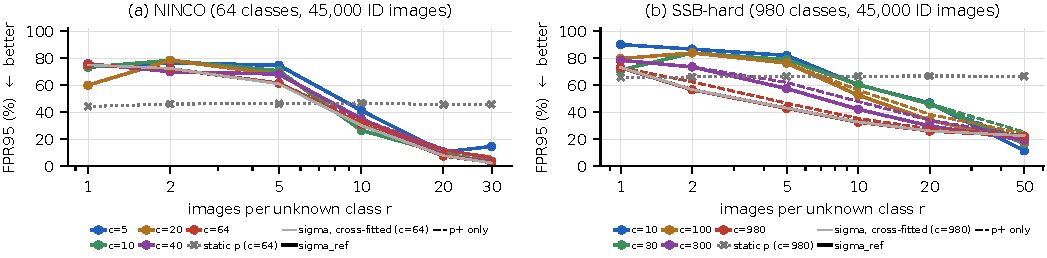
\includegraphics[width=\textwidth]{figs/fig22_rec.pdf}
\caption{再出現と混入率（\FPR{}，単体，DINOv2 L/14 + DINOv3 L/16）．IDの検証画像45,000枚に，NINCO（a）またはSSB-hard（b）から$c$個の未知クラス$\times$$r$枚を加えたテスト集合（クラスと画像の選び方を変えた3回の平均）．実線は$\sR$，破線は$\pP$だけ（参照画像で読む），灰色の点線は静的$p$，灰色の細い実線は交差適合した$\sigma$（後二者は$c$が最大の条件）．}
\label{fig:rec}
\end{figure*}

同じクラスが何枚あり，どの混入率から効くのかを，OpenOODのIDの検証画像45,000枚に，NINCO（64クラス）またはSSB-hard（980クラス，各50枚）から$c$個の未知クラスを$r$枚ずつ加えたテスト集合で実測した（\figref{rec}，全条件は付録\ref{sec:app_rec}）．

\textbf{再出現しない未知には静的な検出器より劣る．}$r\le5$では，$\sR$は同じ特徴の静的$p$より\FPR{}が高く（\NRRecNLeFive{}条件中\NRRecLeFiveWorseStatic{}条件），差の平均は$r{=}1$で\NRRecROneMeanD{}，$r{=}2$で\NRRecRTwoMeanD{}，$r{=}5$で\NRRecRFiveMeanD{}ポイント，最大\NRRecLeFiveMaxD{}ポイントである．NINCOの64クラス$\times$1枚では$\sR$も$\pP$だけも\NRRecNincoCSixtyFourROne\%に対し，静的$p$は\NRRecNincoCSixtyFourROneStatic\%である．1枚だけの未知は$k_g{=}10$本の辺をすべて外へ張るので，伝播はその画像を隣のIDに均す．付録の一つの量$h$は$r\le2$の\NRRecHvsRefLeTwoN{}条件でさらに平均\NRRecHvsRefLeTwoMeanD{}ポイント悪い．$r\ge10$では逆転し（\NRRecNGeTen{}条件中\NRRecGeTenBetterStatic{}条件，差の平均\NRRecGeTenMeanD{}），NINCOの64クラス$\times$10枚で\NRRecNincoCSixtyFourRTen\%，30枚で\NRRecNincoCSixtyFourRThirty\%（静的$p$は\NRRecNincoCSixtyFourRThirtyStatic\%）まで下がる．SSB-hard（兄弟クラス）は遅く，980クラス$\times$10枚で\NRRecSsbCNineEightyRTen\%，50枚で\NRRecSsbCNineEightyRFifty\%である．$\sR$と$\sigma$の差は\NRRecNCells{}条件中\NRRecNWithinOneSig{}条件で1ポイント以内（最大\NRRecMaxAbsDiffSig{}）である．

\textbf{混入率が低いときの種はIDが多い．}混入率1\%未満では，\NRSeedLtOneCellsViews{}のセル$\times$ビューのうち種が選ばれたのは\NRSeedLtOneWithSeeds{}だけで，選ばれたときに種に混じるIDの割合は平均\NRSeedLtOneIdFrac{}（\NRSeedLtOneIdFracMin--\NRSeedLtOneIdFracMax）と水準$q{=}0.2$を超える．種が選ばれない場合を0と数えた偽発見割合（命題3が期待値を抑える量）の平均は\NRSeedLtOneFdpUncond{}，混入率1--10\%で\NRSeedOneToTenFdpUncond{}，10\%以上で\NRSeedGeTenFdpUncond{}で，混入率が高いと水準を超える（較正画像とテスト画像のずれ；\secref{fdp}）．低い混入率でまれに選ばれる種は半分近くがIDであり，種が効くのは同じクラスの未知がそれより多く再出現するときである．

\textbf{分離の上界の実測．}系2の上界は格子の全条件・全未知画像で成り立ち（違反0），上界だけから$\pfin\le0.05$が言える未知の割合は，NINCOの$r{=}30$で\NRBdRefNincoRThirtyCertMin--\NRBdRefNincoRThirtyCertMax\%（実際に$\pfin\le0.05$の割合は\NRBdRefNincoRThirtyActMin--\NRBdRefNincoRThirtyActMax\%），$r\le5$では最大\NRBdRefLeFiveCertMax\%，SSB-hardの$r{=}50$では未知クラスの数とともに\NRBdRefSsbCTenRFiftyCert\%（$c{=}10$）から\NRBdRefSsbCNineEightyRFiftyCert\%（$c{=}980$；実際は\NRBdRefSsbCNineEightyRFiftyAct\%）へ下がる（付録\ref{sec:app_bounds}）．系2は，再出現が多く未知クラスの少ない条件で検知の半分程度をクラスの境界と種への辺から説明するが，未知クラスが多いとほとんど何も言わない．付録の$h$の系A1では，較正画像側の下界で保証される未知は全条件で0である．


\subsection{最終スコアの保証の実測}
\label{sec:fdp}
命題4が仮定する較正画像とIDのテスト画像の交換可能性は，両者がImageNet-1Kの学習画像である開発用分割ではほぼ成り立ち（較正画像はクラスごとに2枚と層化されている），較正画像が学習画像，テスト画像が検証画像のベンチマークでは厳密には成り立たない．開発用分割での$\sR$の$\pfin$の誤警報率$\Pr(\pfin\le\alpha)$は，$\alpha{=}0.05$でdev1 \NRDevOneFprFive{}，dev2 \NRDevTwoFprFive{}，$0.2$で\NRDevOneFprTwenty{}，\NRDevTwoFprTwenty{}，BH法（$q{=}0.2$）の偽発見割合は\NRDevOneBhFdp{}，\NRDevTwoBhFdp{}と水準どおりである．ベンチマークでは$\alpha{=}0.05$で\NRValNearFprFive{}（near），\NRValFarFprFive{}（far），\NRValFourFprFive{}（Four-OOD）と，学習画像と検証画像のずれの分だけ水準を超える（$\sigma$の$\pfin$も\NRValSigNearFprFive{}，\NRValSigFarFprFive{}，\NRValSigFourFprFive）．種に混じるIDの割合も，データセットとビューごとに\NRSeedBenchIdMin--\NRSeedBenchIdMax{}と水準$q{=}0.2$を超える．ベンチマークでの命題3，4の保証は近似である．$\sigma$については較正画像を検証画像から取った交換可能な設定でも，誤警報率が$\alpha{=}0.05$で\NVcalFprZeroZeroFiveMin{}--\NVcalFprZeroZeroFiveMax{}と水準どおりであることを確かめた（付録\ref{sec:app_fdp}）．

\subsection{共変量シフトしたID}
\label{sec:csid}
IDのテスト画像45,000枚に，ImageNet-V2（同じ1,000クラスの新しい検証画像10,000枚）またはImageNet-R（200クラスの絵・彫刻などの描画30,000枚）をIDとして加えた（付録\ref{sec:app_csid}の\tabref{csid}）．ImageNet-V2はIDと区別されず（IDとV2の\AUC{} \NRCsVTwoNearRefIcAuroc\%），V2も受け入れる全体の\FPR{}はnear-OODで\NRCsVTwoNearRefFsFpr\%，far-OODで\NRCsVTwoFarRefFsFpr\%と，同じ実行でIDだけを受け入れる場合（\NRCsVTwoNearRefIoFpr\%，\NRCsVTwoFarRefIoFpr\%）からほとんど変わらない（$\alpha{=}0.05$の誤警報率はV2で\NRCsVTwoNearFprCsFive{}）．ImageNet-Rはほぼすべて未知と判定され（IDとRの\AUC{} \NRCsRNearRefIcAuroc\%，誤警報率\NRCsRNearFprCsFive{}，種の\NRCsRNearSeedShare\%がR），全体の\FPR{}はnear-OODで\NRCsRNearRefFsFpr\%，far-OODで\NRCsRFarRefFsFpr\%に悪化する．同じ特徴の静的$p$はRをIDにより近く扱うので（\AUC{} \NRCsRNearStaticIcAuroc\%），far-OODの全体では\NRCsRFarStaticFsFpr\%と本手法より良い．Salmon Ladderは支持画像の分布からのずれを，意味のずれと共変量のずれの区別なく未知とみなすので，描画のような強い共変量シフトをIDとして受け入れる運用にはそのままでは使えない．

\subsection{ImageNet-200とCIFAR-100}
\label{sec:in200}
\textbf{ImageNet-200．}構成を固定したまま単体で評価した（\NInTwoZeroZeroNDraws{}通りの抽出の平均；付録\ref{sec:app_in200}の\tabref{in200}）．$\sR$はnear-OODで\AUC{} \NRITNearAuroc\%，\FPR{} \NRITNearFpr\%，far-OODで\NRITFarAuroc\%，\NRITFarFpr\%であり，OpenOOD v1.5~\cite{zhang2023openood}の報告値の最良（near \NInTwoZeroZeroBestPubNearAuroc\%／\NInTwoZeroZeroBestPubNearFpr\%，far \NInTwoZeroZeroBestPubFarAuroc\%／\NInTwoZeroZeroBestPubFarFpr\%；ImageNet-200で学習したResNet-18）を大きく上回る．ラベルの数を揃えない基線として，全学習画像258,951枚のkNN（$k{=}50$）とクラス平均（同じ2つの特徴），CLIP ViT-B/16のゼロショットのMCMとNegLabelも測った．kNNは\FPR{} \NInTwoZeroZeroKnnAllKFiveZeroNearFpr\%／\NInTwoZeroZeroKnnAllKFiveZeroFarFpr\%，クラス平均は\NInTwoZeroZeroNcmAllNearFpr\%／\NInTwoZeroZeroNcmAllFarFpr\%で16枚の静的$p$（\NInTwoZeroZeroStaticNearFpr\%／\NInTwoZeroZeroStaticFarFpr\%）と同程度にとどまり，MCMとNegLabelは\NInTwoZeroZeroMcmClipNearFpr\%／\NInTwoZeroZeroMcmClipFarFpr\%，\NInTwoZeroZeroNeglabelClipNearFpr\%／\NInTwoZeroZeroNeglabelClipFarFpr\%である．ラベル付き画像を約80倍使っても伝播の分（$\pP$だけで\NRITNearLpFpr\%／\NRITFarLpFpr\%）は得られない．一方，種は効かない．$\sR$は$\pP$だけよりnearで\NRITNearDLp{} [\NRITNearDLpLo, \NRITNearDLpHi]，farで\NRITFarDLp{}ポイント悪く，LGC-max（\NInTwoZeroZeroLgcNearFpr\%／\NInTwoZeroZeroLgcFarFpr\%）にも及ばない．IDが9,000枚しかなく，SSB-hardでは未知が全画像の\NInTwoZeroZeroMixSsbHard\%を占めるからである（付録\ref{sec:app_in200}）．

\textbf{CIFAR-100．}OpenOOD v1.5のCIFAR-100ベンチマーク（\secref{exp}）で，同じ凍結特徴と学習画像からの16枚（クラスあたり，重ならない6通りの抽出），同じ構成で単体の値を測った（\tabref{cifar}）．$\sR$はnear-OODで\AUC{} \NRCFNearAuroc\%，\FPR{} \NRCFNearFpr\%，far-OODで\NRCFFarAuroc\%，\NRCFFarFpr\%で，報告値（CIFAR-100で学習したResNet-18）の最良であるOE（near \NCifarBestPubNearAuroc\%／\NCifarBestPubNearFpr\%，外れ値データで学習）とRotPred（far \NCifarBestPubFarAuroc\%／\NCifarBestPubFarFpr\%）を\AUC{}で10ポイント以上上回る．全学習画像50,000枚のkNN（\NCifarKnnAllKFiveZeroNearFpr\%／\NCifarKnnAllKFiveZeroFarFpr\%）とクラス平均（\NCifarNcmAllNearFpr\%／\NCifarNcmAllFarFpr\%）は16枚の静的$p$（\NCifarStaticNearFpr\%／\NCifarStaticFarFpr\%）から数ポイント以内にとどまり，$32\times32$の画像ではゼロショットのMCMとNegLabelは弱い（\NCifarMcmClipNearFpr\%／\NCifarMcmClipFarFpr\%，\NCifarNeglabelClipNearFpr\%／\NCifarNeglabelClipFarFpr\%）．ここでも利得は伝播にあり，種は効かない．$\pP$だけで\NRCFNearLpFpr\%／\NRCFFarLpFpr\%，$\sR$との差はfar-OODで\NRCFFarDLp{} [\NRCFFarDLpLo, \NRCFFarDLpHi]ポイントで，未知がMNIST・SVHN・Places365で全画像の\NCifarMixFarHiMin{}--\NCifarMixFarHiMax\%を占めると，割合$q$の種がIDのほぼ全数になって$\pN$は情報を失う．交差適合した$\sigma$では，種の閾値に上限$\tau{=}0.05$を付けた登録済みの規則がこの害をほぼ消した（ImageNet-200 nearで\FPR{} \NInTwoZeroZeroMainNearFpr\%→\NInTwoZeroZeroStoreycNearFpr\%，CIFAR-100 farで\NCifarMainFarFpr\%→\NCifarStoreycFarFpr\%；付録\ref{sec:app_cap}）．$\sR$との組合せは評価していない．


\section{結論}
支持画像の質量をグラフで伝播させ順位（共形$p$値）で読む共形ラベル伝播，自己ラベル付けした種からの負の伝播，参照画像で種を選び読む読み出し$\sR$からなる枠組みSalmon Ladderを提案した．凍結した特徴抽出器とクラスあたり16枚のラベル付き画像だけで，OpenOOD v1.5 ImageNet-1Kのnear-OOD（単体で\AUC{} \NRAloneNearAuroc\%，\FPR{} \NRAloneNearFpr\%），far-OOD，Four-OODで公開の最良値を更新し，ImageNet-200とCIFAR-100でも報告値の最良を上回った．利得の大半はグラフ上の伝播の確率の因子にあり，$\sR$は折なしに読み出しの保証を得て，同じ未知クラスの画像の検知の一部を系2でクラスの境界と種への辺から説明する．\textbf{推す構成．}$\sR$（ベース検出器があれば$s_0\exp\sR$）を推す．IDのテスト画像が1万枚程度と少なく未知が多い集合を含むImageNet-200とCIFAR-100では，種を使わない$\pP$だけ（参照画像で読み，同じ保証を持つ）が$\sR$と同等以上だったので，そうした運用には$\pP$だけを推す．45,000枚のIDに未知を加えた格子では，混入率10\%以上の\NRRecHiMixN{}条件（最大\NRRecHiMixMax\%）すべてで$\sR$が良く，混入率だけでは境目は決まらない．\textbf{限界．}1枚しか現れない未知には静的な検出器より劣り，描画への共変量シフトを未知とみなす．ベンチマークでは較正画像とテスト画像のずれのため保証は近似で，ベース検出器との積は命題4の外にある．開発用分割による構成の細部の選択はテスト集合に移らない．理論が扱うのは有効性と分離の上界で，検知力の全体ではない．


{\makeatletter\@secpenalty=0 \makeatother\begin{thebibliography}{99}
\footnotesize\baselineskip12\h\setlength{\itemsep}{0pt}\setlength{\parskip}{0pt}\setlength{\parsep}{0pt}
\bibitem{radford2021clip} A. Radford et al.: Learning transferable visual models from natural language supervision. \textit{ICML}, 2021.
\bibitem{ming2022mcm} Y. Ming et al.: Delving into out-of-distribution detection with vision-language representations. \textit{NeurIPS}, 2022.
\bibitem{jiang2024neglabel} X. Jiang et al.: Negative label guided OOD detection with pretrained vision-language models. \textit{ICLR}, 2024.
\bibitem{zhang2024adaneg} Y. Zhang and L. Zhang: AdaNeg: Adaptive negative proxy guided OOD detection with vision-language models. \textit{NeurIPS}, 2024.
\bibitem{zhang2026tanl} Y. Zhang et al.: Activation matters: Test-time activated negative labels for OOD detection with vision-language models. \textit{CVPR}, 2026.
\bibitem{xu2026interneg} Z. Xu et al.: Mind the way you select negative texts: Pursuing the distance consistency in OOD detection with VLMs. \textit{CVPR}, 2026.
\bibitem{yang2026tins} Y. Yang et al.: TINS: Test-time ID-prototype-separated negative semantics learning for OOD detection. arXiv:2605.10756, 2026.
\bibitem{zhang2023openood} J. Zhang et al.: OpenOOD v1.5: Enhanced benchmark for out-of-distribution detection. \textit{DMLR}, 2024.
\bibitem{park2023nnguide} J. Park, Y. G. Jung, and A. B. J. Teoh: Nearest neighbor guidance for out-of-distribution detection. \textit{ICCV}, 2023.
\bibitem{li2024moodv2} J. Li et al.: MOODv2: Masked image modeling for out-of-distribution detection. \textit{IEEE TPAMI}, 2024.
\bibitem{caetano2025discopatch} F. Caetano et al.: DisCoPatch: Taming adversarially-driven batch statistics for improved out-of-distribution detection. \textit{ICCV}, 2025.
\bibitem{marandon2024adadetect} A. Marandon, L. Lei, D. Mary, and E. Roquain: Adaptive novelty detection with false discovery rate guarantee. \textit{Ann. Stat.}, 52(1), 2024.
\bibitem{huang2021mos} R. Huang and Y. Li: MOS: Towards scaling out-of-distribution detection for large semantic space. \textit{CVPR}, 2021.
\bibitem{bates2023conformal} S. Bates, E. Cand\`{e}s, L. Lei, Y. Romano, and M. Sesia: Testing for outliers with conformal p-values. \textit{Ann. Stat.}, 51(1):149--178, 2023.
\bibitem{zhou2004lgc} D. Zhou et al.: Learning with local and global consistency. \textit{NIPS}, 2004.
\bibitem{benjamini1995bh} Y. Benjamini and Y. Hochberg: Controlling the false discovery rate: A practical and powerful approach to multiple testing. \textit{J. R. Stat. Soc. B}, 1995.
\bibitem{storey2002} J. D. Storey: A direct approach to false discovery rates. \textit{J. R. Stat. Soc. B}, 2002.
\bibitem{oquab2024dinov2} M. Oquab et al.: DINOv2: Learning robust visual features without supervision. \textit{TMLR}, 2024.
\bibitem{simeoni2025dinov3} O. Sim\'{e}oni et al.: DINOv3. arXiv:2508.10104, 2025.
\bibitem{scott2009novelty} C. Scott and G. Blanchard: Novelty detection: Unlabeled data definitely help. \textit{AISTATS}, pp.~464--471, 2009.
\bibitem{blanchard2010ssnd} G. Blanchard, G. Lee, and C. Scott: Semi-supervised novelty detection. \textit{J. Mach. Learn. Res.}, 11:2973--3009, 2010.
\bibitem{haroush2022statistical} M. Haroush, T. Frostig, R. Heller, and D. Soudry: A statistical framework for efficient out of distribution detection in deep neural networks. \textit{ICLR}, 2022.
\bibitem{liang2024integrative} Z. Liang, M. Sesia, and W. Sun: Integrative conformal p-values for out-of-distribution testing with labelled outliers. \textit{J. R. Stat. Soc. B}, 86(3):671--693, 2024.
\bibitem{liu2019tpn} Y. Liu et al.: Learning to propagate labels: Transductive propagation network for few-shot learning. \textit{ICLR}, 2019.
\bibitem{yang2025oodd} Y. Yang et al.: OODD: Test-time out-of-distribution detection with dynamic dictionary. \textit{CVPR}, 2025.
\bibitem{fan2024rtl} K. Fan et al.: Test-time linear out-of-distribution detection. \textit{CVPR}, pp.~23752--23761, 2024.
\bibitem{yang2023auto} P. Yang, J. Liang, J. Cao, and R. He: AUTO: Adaptive outlier optimization for test-time OOD detection. arXiv:2303.12267, 2023.
\bibitem{sun2022knn} Y. Sun, Y. Ming, X. Zhu, and Y. Li: Out-of-distribution detection with deep nearest neighbors. \textit{ICML}, 2022.
\bibitem{xu2024scale} K. Xu et al.: Scaling for training time and post-hoc out-of-distribution detection enhancement. \textit{ICLR}, 2024.
\end{thebibliography}
}

\clearpage
\onecolumn
\appendix
\makeatletter
\@secpenalty=0 % 付録では節の前で早めに改ページしない
\raggedbottom
\predisplaypenalty=10000 % 数式の直前で改ページしない
% 付録は1段組：図表は浮動させず，本文の流れのその位置に置く（入りきらなければ次のページへ送り，キャプションは本文幅）
\renewenvironment{table}[1][]{\par\addvspace{\medskipamount}\noindent\begin{minipage}{\linewidth}\def\@captype{table}\capwidth\hsize\ecapwidth\hsize\abovecaptionskip\z@\belowcaptionskip1mm\centering}{\end{minipage}\par\addvspace{\medskipamount}}
\renewenvironment{figure}[1][]{\par\addvspace{\medskipamount}\noindent\begin{minipage}{\linewidth}\def\@captype{figure}\capwidth\hsize\ecapwidth\hsize\abovecaptionskip1mm\belowcaptionskip\z@\centering}{\end{minipage}\par\addvspace{\medskipamount}}
\expandafter\let\csname table*\endcsname\table \expandafter\let\csname endtable*\endcsname\endtable
\expandafter\let\csname figure*\endcsname\figure \expandafter\let\csname endfigure*\endcsname\endfigure
\newcommand\appblock{\par\ifdim\dimexpr\pagegoal-\pagetotal\relax<5\baselineskip\newpage\else\medskip\fi} % 見出しだけがページの下に残らないように
\makeatother
% 付録の一つの量 h の定理の名前（付録\ref{sec:app_bounds}でも使う）
\newcommand\TFaces{命題A1}
\newcommand\TLimits{定理A1}
\newcommand\TValid{定理A2}
\newcommand\TEscape{定理A3}
\newcommand\TCapture{定理A4}
\newcommand\CSep{系A1}
\section{命題1，2，4と系1，2の証明}
\label{sec:app_proofs}
\figref{graph}に，本文\secref{graph}のグラフと命題1，2の図を示す．

\begin{figure*}[htbp]
\centering
\scalebox{0.77}{% 図2：ラベル伝播のグラフ．(a) 節点と辺と質量の流れ，(b) 再出現する未知の集合 Q とカット w(Q, \bar Q)，(c) 値の尺度はビュー・テスト集合で変わるが較正順位は同じ物差し．
% 全体の幅は約 17.3 cm（\textwidth = 17.7 cm），高さ約 4.8 cm．文字は \figfont（6.74pt）．
\providecommand{\figfont}{\fontsize{6.74pt}{8pt}\selectfont}
\begin{tikzpicture}[font=\figfont, >={Latex[length=1.3mm]}, x=1cm, y=1cm,
  sup/.style={draw=black, fill=black!75, minimum size=0.22cm, inner sep=0pt},
  idsq/.style={draw=black!55, fill=black!10, minimum size=0.2cm, inner sep=0pt},
  oodA/.style={draw=blue!60!black, fill=blue!35, minimum size=0.23cm, inner sep=0pt, regular polygon, regular polygon sides=3},
  calp/.style={draw=blue!70!black, fill=white, line width=0.6pt, minimum size=0.18cm, inner sep=0pt, circle},
  edge/.style={black!45, line width=0.45pt},
  flow/.style={->, orange!85!black, line width=0.7pt},
  lab/.style={inner sep=1pt, font=\figfont}]
% ================================================================ (a) graph and mass flow
\node[lab, anchor=west, font=\figfont\bfseries] at (0,4.6) {(a) 伝播のグラフ：支持画像の質量 $u^{+}$ が辺を伝わる};
\node[sup] (s1) at (0.7,3.85) {}; \node[sup] (s2) at (1.25,4.1) {}; \node[sup] (s3) at (1.7,3.7) {};
\node[lab, anchor=west] at (1.85,4.15) {支持画像（$y_j{=}1$）};
\node[calp] (c1) at (1.05,3.4) {}; \node[calp] (c2) at (2.1,3.2) {};
\node[idsq] (t1) at (0.5,3.1) {}; \node[idsq] (t2) at (1.45,2.95) {}; \node[idsq] (t3) at (2.45,3.85) {};
\node[idsq] (t4) at (2.85,2.15) {}; \node[calp] (c3) at (3.2,2.85) {};
\node[oodA] (q1) at (3.8,2.35) {}; \node[oodA] (q2) at (4.4,2.65) {}; \node[oodA] (q3) at (4.2,1.95) {}; \node[oodA] (q4) at (4.85,2.2) {};
\foreach \a/\b in {s1/s2, s2/s3, s1/t1, s1/c1, s2/c1, s3/t2, s3/c2, s3/t3, c1/t1, c1/t2, t2/c2, t3/c2, t2/t4, c2/c3, t4/c3, c3/q1, t4/q1, q1/q2, q1/q3, q2/q3, q2/q4, q3/q4, q1/q4}{\draw[edge] (\a) -- (\b);}
\draw[flow] (s1) to[bend right=12] (t1);
\draw[flow] (s3) to[bend left=12] (t3);
\draw[flow] (s3) to[bend right=10] (t2);
\draw[flow, orange!60!black, line width=0.5pt] (t2) to[bend right=8] (t4);
\draw[flow, orange!50!black, line width=0.35pt, densely dashed] (t4) -- (q1);
\node[lab, anchor=north, align=center] at (1.0,2.7) {ID：支持画像に近い\\$u^{+}$ 大 $\Rightarrow p^{+}$ 大};
\node[lab, anchor=north, align=center] at (4.35,1.72) {同じ未知クラス：互いに近い\\$u^{+}$ 小 $\Rightarrow p^{+}$ 小};
\node[lab, anchor=west] at (0.0,0.8) {\tikz{\node[sup]{};}\,支持 \tikz{\node[calp]{};}\,参照・較正 $\mathcal{R},\mathcal{C}$ \tikz{\node[idsq]{};}\,テスト（ID） \tikz{\node[oodA]{};}\,テスト（未知）};
\node[lab, anchor=west, orange!85!black] at (0.0,0.4) {$\rightarrow$ $u^{+}$ の流れ（\eqnref{lp}）．$u^{-}$ も同じ辺を流れる};
% ================================================================ (b) the cut
\begin{scope}[xshift=5.85cm]
\node[lab, anchor=west, font=\figfont\bfseries] at (0,4.6) {(b) 再出現する未知の集合 $Q$ とカット $w(Q,\bar{Q})$};
\node[oodA] (p1) at (1.6,3.2) {}; \node[oodA] (p2) at (2.25,3.55) {}; \node[oodA] (p3) at (2.15,2.8) {}; \node[oodA] (p4) at (2.8,3.15) {}; \node[oodA] (p5) at (2.75,2.5) {};
\node[idsq] (o1) at (0.6,3.8) {}; \node[idsq] (o2) at (0.55,2.6) {}; \node[idsq] (o3) at (3.9,3.8) {}; \node[sup] (o4) at (4.0,2.25) {};
\node[lab, anchor=west] at (4.15,2.25) {支持};
\foreach \a/\b in {p1/p2, p1/p3, p2/p3, p2/p4, p3/p4, p3/p5, p4/p5, p1/p5}{\draw[edge, line width=0.75pt] (\a) -- (\b);}
\draw[edge, densely dotted, line width=0.7pt] (o1) -- (p1); \draw[edge] (o2) -- (p1); \draw[edge, densely dotted, line width=0.7pt] (o3) -- (p4); \draw[edge] (o4) -- (p5);
\draw[red!70!black, densely dashed, line width=0.6pt] (2.2,3.1) ellipse (1.0cm and 0.8cm);
\node[lab, red!70!black, anchor=south] at (2.2,3.95) {$Q$（同じ未知クラス $r$ 枚）};
\node[lab, anchor=west, align=left] at (0.0,1.85) {$Q$ が自ら張る辺（実線）は $r$ とともに減る．外の節点が\\$Q$ を選ぶ辺（点線）は残る．};
\node[lab, anchor=west] at (0.0,1.2) {$\displaystyle\sum_{i\in Q}\sqrt{\delta_i}\,u_i\le\frac{\lambda}{1-\lambda}\cdot\frac{w(Q,\bar{Q})}{\min_{j\in Y}\sqrt{\delta_j}}$\quad（命題2）};
\node[lab, anchor=west, align=left] at (0.0,0.42) {$Q$ の各節点が外へ張る辺は $(k_g-r+1)_+$ 本．\\$w(Q,\bar{Q})$ はこれと点線の和で，再出現は\\前者だけを減らす（$Y{=}\hat{Q}$，$Q{=}$ID なら $u^{-}$ の上界）};
\end{scope}
% ================================================================ (c) scale changes, the calibrated rank does not
\begin{scope}[xshift=11.7cm]
\node[lab, anchor=west, font=\figfont\bfseries] at (0,4.6) {(c) $u$ の尺度はビューやテスト集合で変わる};
\node[lab, blue!70!black, anchor=west] at (0.0,4.15) {順位で読めば閾値（$\mathcal{R}$ の下位 $\varepsilon$ 点）も一緒に動く};
\node[lab, anchor=east] at (1.05,3.5) {ビュー $v_1$};
\node[lab, anchor=east] at (1.05,2.4) {ビュー $v_2$};
\draw[->, black!45] (1.15,3.3) -- (5.0,3.3); \node[lab, anchor=north east, black!65] at (5.05,3.28) {$u^{+}$（右ほど ID らしい）};
\draw[->, black!45] (1.15,2.2) -- (5.0,2.2);
\foreach \x in {2.45,2.9,3.25,3.75,4.1,4.45} {\node[calp] at (\x,3.5) {};}
\node[idsq] at (3.55,3.5) {}; \node[oodA] at (1.6,3.51) {};
\foreach \x in {1.85,2.1,2.3,2.6,2.8,3.0} {\node[calp] at (\x,2.4) {};}
\node[idsq] at (2.48,2.4) {}; \node[oodA] at (1.45,2.41) {};
\draw[blue!70!black, line width=0.8pt] (3.1,3.8) -- (3.1,3.25); \draw[blue!70!black, line width=0.8pt] (2.2,2.7) -- (2.2,2.15);
\node[lab, blue!70!black, anchor=west] at (3.15,3.8) {$\mathcal{R}$ の下位 $\varepsilon$ 点};
\draw[red!70!black, line width=0.8pt] (2.65,3.05) -- (2.65,2.05);
\node[lab, red!70!black, anchor=west, align=left] at (1.15,1.7) {$u^{+}$ の固定閾値（赤線）：$v_2$ では ID が\\下回る．ビューの積も取れない};
\node[lab, anchor=west, align=left] at (0.0,0.6) {命題1：$\bom^{\!\top}\mathbf{u}^{+}=\sum_{j\in\mathcal{S}}\sqrt{\delta_j}$ は支持画像の次数\\だけで決まる（節点 $N$ が増えるほど $u^{+}$ は縮む）};
\end{scope}
\end{tikzpicture}
}
\caption{ラベル伝播のグラフ．(a) 節点は支持画像・ラベル付きの参照画像と較正画像・テスト画像で，各節点をコサイン類似度の上位$k_g$個と結ぶ．支持画像に置いた質量$\mathbf{y}^{+}$が辺を伝わり（\eqnref{lp}），支持画像に近いID画像には多く，互いに近い同じ未知クラスの画像には少ししか届かない．種に置いた質量$\mathbf{y}^{-}$も同じ辺を伝わる．(b) 初期質量を置いた節点を含まない集合$Q$に届く質量は，$Q$と外とを結ぶ辺の重みの和$w(Q,\bar{Q})$で上から抑えられる（命題2）．これには$Q$の節点が自ら張る辺（実線）と外の節点が$Q$へ張る辺（点線）が入り，同じ未知クラスが$r$枚そろうと前者は減るが後者は残り得る．(c) 質量の総和は支持画像の次数だけで決まるので（命題1）$u$の尺度はビューやテスト集合ごとに違うが，ラベル付き画像の$u$も同じ尺度で動くので，その中での順位で読めば閾値もビューの積も同じ物差しに乗る．}
\label{fig:graph}
\end{figure*}

\textbf{命題1の証明}（主張は\secref{mass}）．$\bom=D^{1/2}\mathbf{1}$について
\begin{equation*}
S\bom=D^{-1/2}WD^{-1/2}D^{1/2}\mathbf{1}=D^{-1/2}W\mathbf{1}=D^{-1/2}\boldsymbol{\delta}=\bom
\end{equation*}
であり（$\boldsymbol{\delta}=W\mathbf{1}$は次数のベクトル），$S$は対称なので$\bom^{\top}S=\bom^{\top}$である．\eqnref{lp}に左から$\bom^{\top}$を掛けると
\begin{equation*}
\bom^{\top}\mathbf{u}^{(\ell+1)}
=\lambda\,\bom^{\top}S\,\mathbf{u}^{(\ell)}+(1-\lambda)\,\bom^{\top}\mathbf{y}^{+}
=\lambda\,\bom^{\top}\mathbf{u}^{(\ell)}+(1-\lambda)\,\bom^{\top}\mathbf{y}^{+}
\end{equation*}
となり，$\mathbf{u}^{(0)}=\mathbf{0}$からこの漸化式を解けば
\begin{equation*}
\bom^{\top}\mathbf{u}^{(L)}=(1-\lambda^{L})\,\bom^{\top}\mathbf{y}^{+}=(1-\lambda^{L})\sum_{j\in\mathcal{S}}\sqrt{\delta_j}
\end{equation*}
を得る．$L\to\infty$とすれば収束解の式になる．$\square$

\appblock
\textbf{命題2の証明}（主張は\secref{cut}）．収束解は$\mathbf{u}=\lambda S\mathbf{u}+(1-\lambda)\mathbf{1}_Y$を満たし，$Q\cap Y=\emptyset$なので
\begin{equation*}
\sqrt{\delta_i}\,u_i=\lambda\sum_{j}W_{ij}\,\frac{u_j}{\sqrt{\delta_j}}\qquad(i\in Q)
\end{equation*}
である．$U=\sum_{i\in Q}\sqrt{\delta_i}\,u_i$，$\beta=\max_{j}u_j/\sqrt{\delta_j}$とおく．$i\in Q$で足して$j$が$Q$の内か外かで分けると，$u_j\ge0$と$\sum_{i\in Q}W_{ij}\le\delta_j$から
\begin{align*}
U&=\lambda\sum_{j\in Q}\frac{u_j}{\sqrt{\delta_j}}\sum_{i\in Q}W_{ij}\;+\;\lambda\sum_{i\in Q,\,j\notin Q}W_{ij}\,\frac{u_j}{\sqrt{\delta_j}}\\
&\le\lambda\sum_{j\in Q}\sqrt{\delta_j}\,u_j\;+\;\lambda\,w(Q,\bar{Q})\,\beta
\;=\;\lambda\,U+\lambda\,w(Q,\bar{Q})\,\beta
\end{align*}
を得る．\eqnref{walk}と同じランダムウォークの表現から
\begin{equation*}
\frac{u_j}{\sqrt{\delta_j}}=\mathbb{E}_j\Big[\frac{\mathbf{1}[X_T\in Y]}{\sqrt{\delta_{X_T}}}\Big]\le\frac{1}{\min_{s\in Y}\sqrt{\delta_s}}
\end{equation*}
なので$\beta\le1/\min_{s\in Y}\sqrt{\delta_s}$であり，
\begin{equation*}
(1-\lambda)\,U\le\lambda\,w(Q,\bar{Q})\,\beta\le\lambda\,\frac{w(Q,\bar{Q})}{\min_{s\in Y}\sqrt{\delta_s}}
\end{equation*}
を$1-\lambda$で割れば\eqnref{cond}を得る．$\square$

\appblock
\textbf{命題4の証明}（主張は\secref{ref}）．$\sR$をプール$\mathcal{U}=\mathcal{C}\cup\mathcal{T}$の節点の上の関数とみる．
\begin{itemize}
\item[(1)] それを定めるのは，支持画像$\mathcal{S}$，参照画像$\mathcal{R}$，および「$\mathcal{U}$という節点の集合」だけである．グラフと$\mathbf{u}^{+}$は節点の名札に依らない（\secref{graph}）．$\pP$は固定した$\mathcal{R}$との比較なので各画像の$u^{+}$だけで決まる．種はプールの$\pP$の多重集合から\eqnref{bh}の閾値を決めて選ぶので，どの画像が種になるかは$\mathcal{U}$の画像を対称に扱う．$\mathbf{u}^{-}$と$\tilde{\mathbf{u}}^{-}=\lambda S\mathbf{u}^{-}$も同様で，$\pN$は固定した$\mathcal{R}$との比較である．
\item[(2)] したがって$\sR$は，$\mathcal{U}$の中でどの節点を較正画像と呼ぶかを入れ替えても変わらない．これはAdaDetectの条件(8)である（学習標本を$\mathcal{S}\cup\mathcal{R}$，帰無の較正標本を$\mathcal{C}$，テスト標本を$\mathcal{T}$としたもの．同論文の証明は学習標本を所与とした置換の議論なので，その中身は問わない）．種の候補に較正画像を含めるのはこの対称性のためで，テスト画像だけから種を選ぶと，較正画像とテスト画像を入れ替えたときに種の集合が変わり得て条件(8)が崩れる．
\item[(3)] \eqnref{pfin}の$\pfin$は同論文の経験$p$値(10)である．よって定理3.3から(i)と(ii)のPRDS・超一様性が従い，系3.5と系3.7がFDRの上界を与える．$\square$
\end{itemize}

\appblock
\textbf{系1の証明}（主張は\secref{mass}）．\eqnref{walk}のランダムウォーク（各ステップで確率$1-\lambda$で止まる）で，$Q$から初めて外へ出る時刻を$\tau$とする．

\textit{\eqnref{esc}の上界．}$Q\cap Y=\emptyset$なので，$X_T\in Y$となるには$\tau\le T$が要る．止まる時刻$T$は幾何分布で無記憶だから，強マルコフ性より（$X_\tau\in\partial Q$）
\begin{equation*}
\frac{u_i}{\sqrt{\delta_i}}
=\mathbb{E}_i\Big[\mathbf{1}[\tau\le T]\,\frac{u_{X_\tau}}{\sqrt{\delta_{X_\tau}}}\Big]
\le\Pr\nolimits_i(\tau\le T)\,\max_{j\in\partial Q}\frac{u_j}{\sqrt{\delta_j}}
\end{equation*}
である．$\pi_i=\Pr_i(\tau\le T)$とおいて両辺に$\sqrt{\delta_i}$を掛ければ$u_i\le b_i$である．

\textit{逃げる確率．}最初の1歩で場合を分けると
\begin{equation*}
\pi_i=\lambda\Big(e_i+\sum_{j\in Q}P_{ij}\,\pi_j\Big)\quad(i\in Q),\qquad\text{すなわち}\qquad\boldsymbol{\pi}=\lambda(I-\lambda P_{QQ})^{-1}\mathbf{e}
\end{equation*}
である（$\lambda P_{QQ}$のスペクトル半径は1未満）．$\pi^{*}=\max_{x\in Q}\pi_x$とおくと，$\sum_{j\in Q}P_{xj}=1-e_x$と$e_x\le\bar e_Q$から
\begin{equation*}
\pi^{*}\le\lambda\big(\bar e_Q+(1-\bar e_Q)\,\pi^{*}\big),\qquad\text{すなわち}\qquad
\pi^{*}\le\frac{\lambda\,\bar e_Q}{1-\lambda+\lambda\,\bar e_Q}=\psi(\bar e_Q)
\end{equation*}
を満たす．$\bar e_Q=0$なら$\boldsymbol{\pi}=\mathbf{0}$なので$u^{+}_i=0$である．$\square$

\appblock
\textbf{系2の証明}（主張は\secref{ref}）．$Q$は支持画像を含まないので，系1（$Y=\mathcal{S}$）から$u^{+}_v(y)\le b_v(y)$である．種の各節点$j$では収束解が$u^{-}_v(j)=\lambda(S_vu^{-}_v)(j)+(1-\lambda)\ge1-\lambda$を満たし，$\mathbf{u}^{-}_v\ge\mathbf{0}$なので，$y$が種であってもなくても
\begin{equation*}
\tilde u^{-}_v(y)=\lambda\sum_jS_v(y,j)\,u^{-}_v(j)\ge\lambda\sum_{j\in\hat{Q}_v}\frac{W_v(y,j)}{\sqrt{\delta_v(y)\,\delta_v(j)}}\,(1-\lambda)=c_v(y)
\end{equation*}
である．$\pP_v$は$u^{+}$について非減少，$\pN_v$は$\tilde u^{-}$について非増加なので
\begin{equation*}
\log\pP_v(y)\le\log\pP_v[b_v(y)],\qquad\log\pN_v(y)\le\log\pN_v[c_v(y)]
\end{equation*}
で，ビューで足せば$\sR(y)\le B(y)$を得る．$\pfin$は$\sR$について非減少なので$\pfin(y)\le\bar p(y)$である．交差適合した$\sigma$（付録\ref{sec:app_p17}）では，$y$の折$b$に対して他方の折$\bar b$の較正画像と種で同じ議論をすれば（$y$は折$\bar b$の種ではない），$\sigma(y)\le B(y)$と$\pfin(y)\le(1+|\{c\in\mathcal{C}_b:\sigma(c)\le B(y)\}|)/(|\mathcal{C}_b|+1)$を得る．$\square$

\section{参照画像による読み出しの登録と結果}
\label{sec:app_p17}
\textbf{交差適合した$\sigma$（v18--v21の読み出し）．}ラベル付きの4枚（クラスあたり；$\sigma$ではすべて較正画像として使う）とテスト画像を，画像とは独立に等確率で2つの折$b\in\{1,2\}$に分ける（$n_b=|\mathcal{C}_b|=2{,}000$）．折$b$の種$\hat{Q}_b$は，$\mathcal{T}_b$の画像の$u^{+}$の$\mathcal{C}_b$の中での順位に\eqnref{bh}をかけて選ぶ．折$b$の節点$x\in\mathcal{C}_b\cup\mathcal{T}_b$は，他方の折$\bar b$の較正画像と種で採点し，
\begin{equation*}
\sigma(x)=\sum_v\big[\log\tP_v(x)+\log\tN_v(x)\big],\qquad\pfin(x)=\frac{1+|\{x'\in\mathcal{C}_b:\sigma(x')\le\sigma(x)\}|}{n_b+1}
\end{equation*}
とする（$\tP_v$は$u^{+}_v$の$\mathcal{C}_{\bar b}$の中での順位，$\tN_v$は$u^{-}_{\bar b,v}$の$\mathcal{C}_{\bar b}$の中での逆順位）．$\sigma$は$\mathcal{C}_b\cup\mathcal{T}_b$の中の名札の入れ替えに不変なので（$\hat{Q}_{\bar b}$と$\mathbf{u}^{-}_{\bar b}$は折$\bar b$の画像から決まる），命題4と同じ保証が折ごとに成り立つ．局外関数を一方の標本で推定し他方で評価する交差適合~\cite{chernozhukov2018dml}と同じ構造である．付録の他の節の$\sigma$もこの読み出しで，折は乱数で決める．

\textbf{登録．}$\sR$は，$\sigma$の折を参照画像に置き換える読み出しとして，計算の内容・採否の規則・記述的な解析（\tabref{dec}の分解，系2と系A1の格子での実測，共変量シフト）を登録文書（\texttt{experiments/phase17/prereg\_p17.json}，SHA-256 \texttt{068dd4d9}$\cdots$）に記してから実行した．クラスあたりの4枚のうち並びの位置で最初の2枚を参照画像，残り2枚を較正画像とし（付録\ref{sec:app_h16}の$h$と同じ分割），自由な値はない．登録の前に行ったのは，ImageNet-V2とImageNet-Rの特徴抽出（スコアなし），動作確認（dev1の1課題での$\sigma$の値の再現と$\sR$の種の数と$\hat\pi_0$，格子の1課題での上界の違反の数；$\sR$の指標は計算していない），既存の結果の解析（\tabref{devtest}と折の割り当ての確認）である．登録文書は2026年10月11日15:21 UTCに計算サーバに置き，公開リポジトリのブランチ\texttt{phase12-15-registrations}（コミット\texttt{ee565d8}）で公開されたことを15:25 UTCに確かめてから実行した（15:25--15:39 UTC）．登録した集計スクリプトはファイル名の解釈の誤り（\texttt{rep0}の先頭の\texttt{r}を$r$の値と読む）で出力の前に止まったので，その1行だけを直したもの（\texttt{ana17\_fix.py}）で集計した．計算する量は同じで，それ以外の変更と登録からの逸脱はない（\texttt{experiments/phase17/prereg\_p17\_outcome.json}）．

\textbf{採否と結果．}\tabref{dev}に，採否の規則を当てたdev2，記述的に報告するdev1，ベンチマークでの$\sR$と$\sigma$を示す．dev2で規則が成り立ったので$\sR$が主構成になり，ベンチマークの値は計算されたとおりに報告している．ベンチマークでは，$\sR$はImageNet-1Kのnear-OODで$\sigma$より良く（単体\NRAloneNearDSig{} [\NRAloneNearDSigLo, \NRAloneNearDSigHi]，$\times$TINS \NRTinsNearDSig{}），他の設定では区間が0を含む．開発用分割ではdev1のnearでも\NRDevOneNearD{} [\NRDevOneNearDLo, \NRDevOneNearDHi]と良い．

\begin{table}[htbp]
\centering
\caption{参照画像による読み出し$\sR$と交差適合した$\sigma$（単体，dev1とdev2は5通り，ベンチマークは6通りの抽出の平均；差は$\sR-\sigma$，抽出を単位とする対応のある95\% $t$区間）．dev2の2行が登録した採否の規則の対象（区間の上端が+0.5以下）．}
\label{tab:dev}
\vspace{1.5mm}
{\fontsize{6.5pt}{7.6pt}\selectfont\renewcommand{\arraystretch}{1.0}%
\setlength{\tabcolsep}{2.2pt}\begin{tabular}{@{}lcc|cc|c@{}}
\hline
\rule[-2.0pt]{0pt}{8.6pt} & \multicolumn{2}{c|}{$\sigma$（交差適合）} & \multicolumn{2}{c|}{$\sR$（本稿）} & \\
\rule[-2.0pt]{0pt}{8.6pt}設定 & \AUC & \FPR & \AUC & \FPR & \FPR{}の差 [95\%区間] \\
\hline
dev2 near（採否の規則） & 97.16 & 12.92 & 97.19 & 12.94 & +0.02 [-0.18, +0.21] \\
dev2 far（採否の規則） & 96.56 & 16.73 & 96.56 & 16.65 & -0.08 [-0.50, +0.34] \\
dev1 near & 97.08 & 13.75 & 97.11 & 13.50 & -0.25 [-0.43, -0.07] \\
dev1 far & 96.70 & 16.51 & 96.66 & 16.51 & +0.00 [-0.86, +0.86] \\
\hline
ImageNet-1K near-OOD & 97.94 & 11.50 & 97.98 & 11.26 & -0.24 [-0.34, -0.15] \\
ImageNet-1K far-OOD & 98.79 & 5.17 & 98.81 & 5.14 & -0.03 [-0.08, +0.01] \\
Four-OOD & 98.80 & 4.56 & 98.81 & 4.55 & -0.01 [-0.07, +0.04] \\
ImageNet-200 near-OOD & 98.17 & 9.07 & 98.22 & 8.68 & -0.39 [-1.06, +0.29] \\
ImageNet-200 far-OOD & 99.35 & 2.15 & 99.40 & 2.06 & -0.09 [-0.23, +0.06] \\
CIFAR-100 near-OOD & 99.18 & 2.90 & 99.20 & 2.90 & +0.01 [-0.09, +0.10] \\
CIFAR-100 far-OOD & 99.37 & 2.34 & 99.37 & 2.48 & +0.14 [-0.69, +0.98] \\
\hline
ImageNet-1K near-OOD $\times$TINS & 98.09 & 10.50 & 98.13 & 10.21 & -0.28 [-0.36, -0.20] \\
ImageNet-1K far-OOD $\times$TINS & 99.05 & 4.16 & 99.06 & 4.14 & -0.02 [-0.07, +0.02] \\
Four-OOD $\times$TINS & 99.09 & 3.39 & 99.09 & 3.39 & -0.00 [-0.04, +0.04] \\
\hline
\end{tabular}}%

\end{table}

\textbf{種．}\tabref{seeds}に，ベンチマークで$\sR$に選ばれた種（登録した記録；ビューごと，6通りの抽出の平均）を示す．種に混じるIDの割合は\NRSeedBenchIdMin--\NRSeedBenchIdMax{}と水準$q{=}0.2$を超え，較正画像も種に選ばれる（SSB-hardでは未知がプールの半分を占め，種がプールの6割を超える）．

\begin{table}[htbp]
\centering
\caption{学習画像の較正で$\sR$に選ばれた種（ビューごと，6通りの抽出の平均）．種は種の数，プール\%はプール$\mathcal{U}=\mathcal{C}\cup\mathcal{T}$に占める割合，較正は種になった較正画像の数（2,000枚中），ID率は種に混じっていたIDの割合（実測の偽発見割合，水準$q{=}0.2$）．}
\label{tab:seeds}
\vspace{1.5mm}
{\fontsize{6.5pt}{7.6pt}\selectfont\renewcommand{\arraystretch}{1.0}%
\setlength{\tabcolsep}{2.8pt}\begin{tabular}{@{}l|rrrr|rrrr@{}}
\hline
\rule[-2.0pt]{0pt}{8.2pt} & \multicolumn{4}{c|}{DINOv2 L/14} & \multicolumn{4}{c}{DINOv3 L/16} \\
\rule[-2.0pt]{0pt}{8.2pt}データセット & 種 & プール\% & 較正 & ID率 & 種 & プール\% & 較正 & ID率 \\
\hline
SSB-hard & 60,412 & 62.9 & 522 & 0.216 & 61,744 & 64.3 & 552 & 0.228 \\
NINCO & 7,420 & 14.0 & 58 & 0.241 & 7,855 & 14.9 & 70 & 0.271 \\
iNaturalist & 13,191 & 23.1 & 113 & 0.243 & 13,515 & 23.7 & 124 & 0.261 \\
Textures & 5,995 & 11.5 & 47 & 0.237 & 6,488 & 12.4 & 60 & 0.272 \\
OpenImage-O & 18,511 & 29.4 & 153 & 0.226 & 19,594 & 31.2 & 171 & 0.250 \\
iNat.（Four-OOD） & 13,184 & 21.3 & 103 & 0.243 & 13,766 & 22.2 & 118 & 0.275 \\
SUN & 12,509 & 20.2 & 90 & 0.232 & 13,268 & 21.4 & 109 & 0.263 \\
Places & 10,879 & 17.5 & 81 & 0.234 & 11,867 & 19.1 & 100 & 0.259 \\
Textures（Four-OOD） & 6,369 & 11.0 & 44 & 0.230 & 6,939 & 12.0 & 56 & 0.270 \\
\hline
\end{tabular}}%

\end{table}

\textbf{$\sigma$の開発用分割の値が表ごとに違う理由．}$\sigma$は折の乱数に依存する．\tabref{selq}（第2段の選択）の$\sigma$は，各抽出で3通りのTINSの順序ごとに位置で折を割り当てた値の平均（dev1 \NRFcDevOneNearPFourteen\%／\NRFcDevOneFarPFourteen\%，dev2 \NRFcDevTwoNearPFourteen\%／\NRFcDevTwoFarPFourteen\%；near／far）で，\tabref{dev}と付録\ref{sec:app_h16}の\tabref{h16}の値は画像の番号順に1通りの折を割り当てたもの（dev1 \NRFcDevOneNearPSixteen\%／\NRFcDevOneFarPSixteen\%，dev2 \NRFcDevTwoNearPSixteen\%／\NRFcDevTwoFarPSixteen\%）である．同じ抽出で折の割り当てを4通り（第14段階の3通りと番号順の1通り）に変えたときの値の範囲は1抽出あたり平均\NRFcRangeFourMean{}，最大\NRFcRangeFourMax{}ポイント（番号順の値と3通りの平均の差は最大\NRFcDevSixteenMax{}ポイント）で，表どうしの違いはこの揺れに収まる．付録\ref{sec:app_h16res}の探索の段落の$\sigma$（dev1 \NHsExplSigNear\%／\NHsExplSigFar\%）は，探索時のコードでのさらに別の割り当ての値である．$\sR$は乱数を含まないので，この揺れはない．

\section{開発用分割とテスト集合の一致}
\label{sec:app_devtest}
\tabref{devtest}に，$\sigma$の第2段の\NRDtNCand{}候補の開発用分割（dev1，dev2；5通りの抽出，折は3通りの平均）とテスト集合（OpenOOD v1.5 ImageNet-1K，6通りの抽出）での\FPR{}を示す（単体；既存の結果の解析で，登録外）．dev1とdev2の順位相関はnear \NRDtNearSpDevOneDevTwo{}，far \NRDtFarSpDevOneDevTwo{}と高いが，dev2とテストではnear \NRDtNearSpDevTwoTest{}，far \NRDtFarSpDevTwoTest{}（dev1とテストでは\NRDtNearSpDevOneTest{}，\NRDtFarSpDevOneTest{}）に下がる．候補の対のうち差の符号がdev2とテストで一致するのはnear \NRDtNearPairAgree{}，far \NRDtFarPairAgree{}で，選ばれた統計量$\pP\pN$の6候補に限ると順位相関はnear \NRDtNearSpPpOnly{}，far \NRDtFarSpPpOnly{}である．静的$p$を加えたときの向き（nearで悪くfarで良い）は再現するが，$q$の差は開発用分割で数ポイントあっても再現しない（$q{=}0.05$はdev1のnearで$q{=}0.2$より約4ポイント悪いが，テストでは良い）．種の規則の差も再現しない．dev1で選んだ候補（Storey型，$q{=}0.2$，$\pP\pN$）はテストのnearで\NRDtNCand{}候補中\NRDtNearRankOnTest{}位，farで\NRDtFarRankChosen{}位である（dev1のfarで最良の候補はテストのfarで\NRDtFarRankOnTest{}位）．dev1とdev2はどちらもImageNet-1Kの学習画像から作った分割でfar-OODの画像集合も共通であり，学習画像と検証画像のずれやOpenOODのOOD集合の性質を含まない．付録\ref{sec:app_h16}の$h$がdev2で非劣，テスト集合のImageNet-1Kで単体\NRHsTestMinDiff--\NRHsTestMaxDiff{}ポイント，$\times$TINSのnearで\NRHsTestTinsNearDiff{}ポイント悪かったのも同じ限界の表れである．

\begin{table}[htbp]
\centering
\caption{$\sigma$の第2段の候補の開発用分割とテスト集合での\FPR{}（単体）．順位はテスト集合での順位（\NRDtNCand{}候補中）．行はdev1 nearの昇順．}
\label{tab:devtest}
\vspace{1.5mm}
{\fontsize{6.4pt}{7.5pt}\selectfont\renewcommand{\arraystretch}{1.0}%
\setlength{\tabcolsep}{2.4pt}\begin{tabular}{@{}l|cccc|cccc@{}}
\hline
\rule[-2.0pt]{0pt}{8.2pt} & \multicolumn{4}{c|}{near（\FPR{}[\%]）} & \multicolumn{4}{c}{far（\FPR{}[\%]）} \\
\rule[-2.0pt]{0pt}{8.2pt}候補（$\sigma$，dev1の順） & dev1 & dev2 & テスト & 順位 & dev1 & dev2 & テスト & 順位 \\
\hline
Storey型，$q{=}0.2$，$\pP\pN$ & 13.54 & 13.09 & 11.50 & 10 & 16.60 & 17.00 & 5.17 & 18 \\
Storey型，$q{=}0.2$，$\min(\cdot)$ & 13.74 & 13.21 & 11.49 & 9 & 15.71 & 16.12 & 5.17 & 17 \\
単純BH，$q{=}0.2$，$\pP\pN$ & 13.82 & 13.40 & 11.00 & 1 & 16.79 & 16.99 & 4.96 & 14 \\
単純BH，$q{=}0.2$，$\min(\cdot)$ & 13.98 & 13.53 & 11.01 & 2 & 15.80 & 16.15 & 4.96 & 13 \\
Storey型，$q{=}0.1$，$\pP\pN$ & 14.60 & 14.33 & 11.01 & 4 & 18.03 & 17.75 & 4.78 & 11 \\
Storey型，$q{=}0.1$，$\min(\cdot)$ & 14.72 & 14.41 & 11.01 & 3 & 16.54 & 16.32 & 4.80 & 12 \\
単純BH，$q{=}0.1$，$\pP\pN$ & 15.15 & 15.22 & 11.40 & 7 & 18.98 & 17.81 & 4.70 & 7 \\
単純BH，$q{=}0.1$，$\min(\cdot)$ & 15.31 & 15.32 & 11.44 & 8 & 16.93 & 16.38 & 4.71 & 8 \\
Storey型，$q{=}0.2$，$\pP\pN\times$静的$p$ & 16.31 & 15.30 & 12.57 & 13 & 11.26 & 11.46 & 4.48 & 5 \\
単純BH，$q{=}0.2$，$\pP\pN\times$静的$p$ & 16.54 & 15.58 & 12.31 & 12 & 11.27 & 11.45 & 4.39 & 4 \\
Storey型，$q{=}0.1$，$\pP\pN\times$静的$p$ & 17.44 & 16.46 & 12.30 & 11 & 11.79 & 11.78 & 4.30 & 2 \\
Storey型，$q{=}0.05$，$\pP\pN$ & 17.76 & 18.10 & 11.32 & 5 & 20.62 & 19.74 & 4.74 & 10 \\
単純BH，$q{=}0.1$，$\pP\pN\times$静的$p$ & 17.98 & 17.23 & 12.96 & 17 & 12.08 & 11.84 & 4.28 & 1 \\
Storey型，$q{=}0.05$，$\min(\cdot)$ & 18.04 & 18.18 & 11.37 & 6 & 16.82 & 15.64 & 4.73 & 9 \\
単純BH，$q{=}0.05$，$\pP\pN$ & 19.71 & 19.98 & 12.84 & 14 & 19.60 & 19.47 & 5.06 & 16 \\
単純BH，$q{=}0.05$，$\min(\cdot)$ & 20.01 & 20.07 & 12.91 & 15 & 16.12 & 15.45 & 5.03 & 15 \\
Storey型，$q{=}0.05$，$\pP\pN\times$静的$p$ & 20.97 & 19.65 & 12.94 & 16 & 12.55 & 12.50 & 4.34 & 3 \\
単純BH，$q{=}0.05$，$\pP\pN\times$静的$p$ & 22.97 & 21.21 & 14.20 & 18 & 12.40 & 12.47 & 4.53 & 6 \\
\hline
\end{tabular}}%

\end{table}

\section{二つの因子の詳細}
\label{sec:app_dec}
\tabref{dec}の因子をOpenOODのデータセット別に見ると，密度の因子$\sqrt{\delta}$だけの\AUC{}はSSB-hard \NRDecDegSsbHardAuroc\%，NINCO \NRDecDegNincoAuroc\%，iNaturalist \NRDecDegInatAuroc\%，Textures \NRDecDegTexturesAuroc\%，OpenImage-O \NRDecDegOpenimageoAuroc\%で，SSB-hard，NINCO，iNaturalistでは未知の方が密，Texturesでは差がなく，OpenImage-OではIDの方が密である．確率の因子$q$だけの\FPR{}と積$u^{+}$の\FPR{}は，SSB-hardで\NRDecQSsbHardFpr\%と\NRDecUSsbHardFpr\%，NINCOで\NRDecQNincoFpr\%と\NRDecUNincoFpr\%，iNaturalistで\NRDecQInatFpr\%と\NRDecUInatFpr\%，Texturesで\NRDecQTexturesFpr\%と\NRDecUTexturesFpr\%，OpenImage-Oで\NRDecQOpenimageoFpr\%と\NRDecUOpenimageoFpr\%である．付録\ref{sec:app_h16res}の探索（dev1）では次数だけの\AUC{}がfar-OODで80\%を超えたが，テスト集合では再現しなかった．密度の因子は単独の手がかりとしてではなく，確率の因子と組んで未知の塊の内側の質量を薄める形で効くと解釈できる．$\sigma$の読み出しの順位を$u^{\pm}/\sqrt{\delta}$で取ると（\tabref{dec}の4行目），ImageNet-1Kではnearでもfarでも$\sigma$より悪い．

\section{分離の上界の実測}
\label{sec:app_bounds}
\tabref{bounds}に，\secref{rec}の格子の各条件（3回の平均）で，系2の上界から$\pfin\le0.05$が言える未知の割合（保証），実際に$\pfin\le0.05$の割合（実），$\sR$での上界の余裕$B(y)-\sR(y)$の中央値（対数），付録の$h$の系A1（\TCapture{}の較正画像側の下界$\ell=\rho\omega$で読んだ割合（下界），実際の較正画像のスコア$s$で読んだ割合（実較正），実際に$p\le0.05$の割合（実），$\pi_Q/\bar\phi$と較正画像での$\ell/s$の中央値）を示す（登録した記述的な計算で，何も選ばない）．上界はすべての未知画像で成り立つ（系2の$\sR$と$\sigma$，系A1の$h\le\pi_Q$と$\pi_Q\le\bar\phi$のいずれも違反0）．$\sR$の系2はNINCOの$r{=}30$で実際の検知の約半分を保証し，$r\le5$ではほとんど保証しない．SSB-hardの$r{=}50$では保証の割合は未知クラスの数とともに下がる（$c{=}10$で\NRBdRefSsbCTenRFiftyCert\%，$c{=}980$で\NRBdRefSsbCNineEightyRFiftyCert\%）．余裕の中央値は\NRBdRefSlackMin--\NRBdRefSlackMax{}で，緩さの源は，系1が出口の質量を最大値で押さえること（$b_v$）と，種への辺だけを数えて種から2歩以上離れた質量を捨てること（$c_v$）である．$h$の系A1では，較正画像側の下界$\ell$が実際のスコア$s$の\NRBdHOneEllOverSMedMin--\NRBdHOneEllOverSMedMax{}倍（中央値）しかないので，下界で読むと保証される未知は全条件で0になり，実際のスコアで読めば最大\NRBdHOneCertSMax\%を保証する．

\begin{table}[htbp]
\centering
\caption{分離の上界の実測（格子の各条件，3回の平均；[\%]，余裕と比は中央値）．保証：上界だけから$\pfin\le0.05$（$h$では$p\le0.05$）が言える未知の割合，実：実際の割合．}
\label{tab:bounds}
\vspace{1.5mm}
{\fontsize{6.2pt}{7.2pt}\selectfont\renewcommand{\arraystretch}{1.0}%
\setlength{\tabcolsep}{2.2pt}\begin{tabular}{@{}lrr|ccc|cc|ccccc@{}}
\hline
\rule[-2.0pt]{0pt}{8.2pt} & & & \multicolumn{3}{c|}{$\sR$（系2）} & \multicolumn{2}{c|}{$\sigma$（系2）} & \multicolumn{5}{c}{$h$（系A1）} \\
\rule[-2.0pt]{0pt}{8.2pt}未知 & $c$ & $r$ & 保証 & 実 & 余裕 & 保証 & 実 & 下界 & 実較正 & 実 & $\pi/\bar\phi$ & $\ell/s$ \\
\hline
NINCO & 5 & 1 & 0.0 & 33.3 & 3.2 & 0.0 & 33.3 & 0.0 & 0.0 & 20.0 & 1.00 & 0.31 \\
NINCO & 5 & 2 & 0.0 & 26.7 & 3.2 & 0.0 & 26.7 & 0.0 & 0.0 & 6.7 & 1.00 & 0.31 \\
NINCO & 5 & 5 & 0.0 & 28.0 & 4.0 & 0.0 & 28.0 & 0.0 & 0.0 & 36.0 & 0.97 & 0.31 \\
NINCO & 5 & 10 & 22.7 & 64.0 & 4.8 & 26.7 & 63.3 & 0.0 & 4.0 & 67.3 & 0.90 & 0.31 \\
NINCO & 5 & 20 & 40.3 & 91.0 & 5.6 & 43.3 & 91.7 & 0.0 & 39.2 & 83.3 & 0.63 & 0.31 \\
NINCO & 5 & 30 & 47.1 & 87.6 & 6.0 & 55.8 & 90.7 & 0.0 & 8.5 & 70.8 & 0.79 & 0.31 \\
NINCO & 10 & 1 & 0.0 & 40.0 & 3.7 & 0.0 & 36.7 & 0.0 & 0.0 & 20.0 & 1.00 & 0.31 \\
NINCO & 10 & 2 & 3.3 & 25.0 & 3.3 & 3.3 & 25.0 & 0.0 & 0.0 & 11.7 & 1.00 & 0.31 \\
NINCO & 10 & 5 & 0.0 & 33.3 & 4.1 & 0.0 & 32.7 & 0.0 & 0.0 & 33.3 & 0.97 & 0.31 \\
NINCO & 10 & 10 & 17.3 & 78.7 & 6.0 & 24.0 & 77.0 & 0.0 & 15.1 & 86.1 & 0.85 & 0.31 \\
NINCO & 10 & 20 & 48.5 & 92.3 & 7.0 & 55.7 & 92.8 & 0.0 & 30.6 & 61.5 & 0.81 & 0.31 \\
NINCO & 10 & 30 & 53.2 & 98.0 & 8.5 & 58.4 & 98.9 & 0.0 & 45.1 & 83.3 & 0.72 & 0.31 \\
NINCO & 20 & 1 & 5.0 & 48.3 & 3.8 & 5.0 & 48.3 & 0.0 & 0.0 & 20.0 & 1.00 & 0.31 \\
NINCO & 20 & 2 & 0.0 & 28.3 & 3.5 & 0.0 & 28.3 & 0.0 & 0.0 & 10.8 & 1.00 & 0.31 \\
NINCO & 20 & 5 & 0.0 & 41.0 & 4.1 & 0.0 & 39.0 & 0.0 & 0.0 & 45.7 & 0.97 & 0.31 \\
NINCO & 20 & 10 & 10.0 & 68.3 & 5.9 & 14.0 & 68.2 & 0.0 & 9.0 & 65.5 & 0.87 & 0.31 \\
NINCO & 20 & 20 & 44.2 & 93.3 & 7.7 & 48.8 & 93.3 & 0.0 & 27.3 & 72.4 & 0.82 & 0.31 \\
NINCO & 20 & 30 & 56.6 & 97.3 & 9.0 & 65.6 & 97.3 & 0.0 & 7.9 & 69.0 & 0.82 & 0.31 \\
NINCO & 40 & 1 & 5.8 & 28.3 & 3.2 & 5.0 & 27.5 & 0.0 & 0.0 & 9.2 & 1.00 & 0.31 \\
NINCO & 40 & 2 & 0.8 & 37.5 & 3.9 & 0.8 & 37.5 & 0.0 & 0.0 & 22.1 & 1.00 & 0.31 \\
NINCO & 40 & 5 & 1.3 & 40.2 & 4.2 & 1.2 & 39.2 & 0.0 & 0.0 & 39.5 & 0.96 & 0.31 \\
NINCO & 40 & 10 & 14.2 & 70.9 & 6.5 & 18.1 & 68.5 & 0.0 & 6.5 & 65.8 & 0.88 & 0.31 \\
NINCO & 40 & 20 & 44.5 & 94.5 & 9.1 & 49.8 & 93.0 & 0.0 & 22.3 & 70.4 & 0.81 & 0.31 \\
NINCO & 40 & 30 & 57.9 & 97.9 & 12.1 & 61.2 & 98.2 & 0.0 & 22.5 & 65.3 & 0.80 & 0.31 \\
NINCO & 64 & 1 & 3.6 & 27.6 & 3.3 & 3.6 & 27.1 & 0.0 & 0.0 & 12.5 & 1.00 & 0.31 \\
NINCO & 64 & 2 & 2.9 & 34.1 & 3.6 & 3.1 & 34.1 & 0.0 & 0.0 & 23.2 & 1.00 & 0.31 \\
NINCO & 64 & 5 & 3.3 & 44.4 & 4.4 & 4.2 & 44.6 & 0.0 & 0.0 & 46.7 & 0.97 & 0.31 \\
NINCO & 64 & 10 & 17.5 & 74.8 & 7.9 & 21.5 & 74.1 & 0.0 & 9.3 & 64.4 & 0.88 & 0.31 \\
NINCO & 64 & 20 & 46.2 & 94.8 & 11.1 & 49.7 & 94.6 & 0.0 & 18.6 & 71.7 & 0.83 & 0.31 \\
NINCO & 64 & 30 & 56.6 & 98.0 & 12.6 & 55.0 & 98.5 & 0.0 & 29.7 & 74.8 & 0.76 & 0.31 \\
SSB-hard & 10 & 1 & 0.0 & 10.0 & 2.2 & 0.0 & 10.0 & 0.0 & 0.0 & 0.0 & 1.00 & 0.31 \\
SSB-hard & 10 & 2 & 0.0 & 18.3 & 3.0 & 0.0 & 18.3 & 0.0 & 0.0 & 5.0 & 1.00 & 0.31 \\
SSB-hard & 10 & 5 & 0.0 & 24.7 & 3.8 & 0.0 & 24.0 & 0.0 & 0.0 & 22.7 & 0.96 & 0.31 \\
SSB-hard & 10 & 10 & 7.0 & 44.7 & 4.1 & 7.0 & 44.3 & 0.0 & 9.7 & 43.3 & 0.89 & 0.31 \\
SSB-hard & 10 & 20 & 16.3 & 56.3 & 3.9 & 21.8 & 57.0 & 0.0 & 13.8 & 48.5 & 0.88 & 0.31 \\
SSB-hard & 10 & 50 & 37.9 & 89.9 & 9.9 & 42.7 & 90.3 & 0.0 & 9.8 & 53.9 & 0.82 & 0.31 \\
SSB-hard & 30 & 1 & 1.1 & 37.8 & 2.9 & 1.1 & 36.7 & 0.0 & 0.0 & 15.6 & 1.00 & 0.31 \\
SSB-hard & 30 & 2 & 0.0 & 22.2 & 2.8 & 0.0 & 21.1 & 0.0 & 0.0 & 12.8 & 1.00 & 0.31 \\
SSB-hard & 30 & 5 & 2.0 & 24.0 & 2.8 & 2.2 & 23.6 & 0.0 & 0.0 & 26.4 & 0.97 & 0.31 \\
SSB-hard & 30 & 10 & 3.6 & 44.4 & 4.4 & 6.8 & 44.4 & 0.0 & 2.8 & 47.7 & 0.92 & 0.31 \\
SSB-hard & 30 & 20 & 22.3 & 57.1 & 5.8 & 23.3 & 59.7 & 0.0 & 5.0 & 40.7 & 0.89 & 0.31 \\
SSB-hard & 30 & 50 & 29.3 & 86.0 & 11.1 & 31.6 & 86.9 & 0.0 & 6.0 & 46.9 & 0.84 & 0.31 \\
SSB-hard & 100 & 1 & 2.0 & 23.3 & 2.5 & 2.0 & 23.7 & 0.0 & 0.0 & 11.7 & 1.00 & 0.31 \\
SSB-hard & 100 & 2 & 0.7 & 20.2 & 2.6 & 0.7 & 19.8 & 0.0 & 0.0 & 13.3 & 1.00 & 0.31 \\
SSB-hard & 100 & 5 & 1.7 & 29.9 & 3.3 & 2.4 & 29.3 & 0.0 & 0.0 & 28.2 & 0.97 & 0.31 \\
SSB-hard & 100 & 10 & 8.6 & 50.7 & 6.4 & 11.0 & 53.6 & 0.0 & 2.4 & 31.0 & 0.93 & 0.31 \\
SSB-hard & 100 & 20 & 22.5 & 70.2 & 10.1 & 24.7 & 71.4 & 0.0 & 6.0 & 35.8 & 0.90 & 0.31 \\
SSB-hard & 100 & 50 & 18.4 & 84.5 & 12.3 & 18.2 & 84.3 & 0.0 & 7.0 & 41.3 & 0.81 & 0.31 \\
SSB-hard & 300 & 1 & 2.6 & 26.8 & 2.4 & 2.3 & 26.4 & 0.0 & 0.0 & 15.8 & 1.00 & 0.31 \\
SSB-hard & 300 & 2 & 2.3 & 30.9 & 3.0 & 2.3 & 30.4 & 0.0 & 0.0 & 24.3 & 1.00 & 0.31 \\
SSB-hard & 300 & 5 & 10.2 & 46.3 & 5.8 & 9.5 & 45.5 & 0.0 & 1.2 & 33.2 & 0.96 & 0.31 \\
SSB-hard & 300 & 10 & 15.5 & 61.8 & 9.6 & 15.6 & 61.8 & 0.0 & 3.1 & 33.6 & 0.93 & 0.31 \\
SSB-hard & 300 & 20 & 11.9 & 74.1 & 11.6 & 12.1 & 74.5 & 0.0 & 2.1 & 25.1 & 0.89 & 0.31 \\
SSB-hard & 300 & 50 & 4.4 & 84.0 & 13.5 & 4.3 & 83.5 & 0.0 & 0.3 & 3.8 & 0.78 & 0.33 \\
SSB-hard & 980 & 1 & 5.9 & 32.5 & 2.8 & 5.7 & 32.0 & 0.0 & 0.6 & 24.9 & 1.00 & 0.31 \\
SSB-hard & 980 & 2 & 10.9 & 47.2 & 5.5 & 10.9 & 46.9 & 0.0 & 0.6 & 34.0 & 1.00 & 0.31 \\
SSB-hard & 980 & 5 & 14.0 & 61.8 & 9.5 & 13.8 & 61.8 & 0.0 & 1.6 & 30.8 & 0.96 & 0.31 \\
SSB-hard & 980 & 10 & 8.4 & 71.1 & 11.4 & 8.2 & 71.1 & 0.0 & 0.8 & 14.2 & 0.93 & 0.32 \\
SSB-hard & 980 & 20 & 3.8 & 78.3 & 13.2 & 3.9 & 77.8 & 0.0 & 0.0 & 0.1 & 0.86 & 0.33 \\
SSB-hard & 980 & 50 & 0.6 & 81.1 & 13.8 & 0.7 & 79.4 & 0.0 & 0.0 & 0.0 & 0.88 & 0.42 \\
\hline
\end{tabular}}%

\end{table}

\section{共変量シフトしたID}
\label{sec:app_csid}
\tabref{csid}に\secref{csid}の値を示す（登録した記述的な計算；6通りの抽出の平均，単体，学習画像の較正）．テスト集合はIDの検証画像45,000枚，シフトしたID（ImageNet-V2 matched-frequencyの10,000枚またはImageNet-Rの30,000枚），OpenOODのOOD集合1つからなり，ベース検出器のスコアはこれらの画像にないので単体だけを測った．「全体」はIDとシフトしたIDの両方を受け入れるときの\AUC{}と\FPR{}，「シフト対OOD」はシフトしたIDとOODだけ，「ID対OOD」は同じ実行のIDとOODだけ，「ID対シフト」はIDとシフトしたIDを見分ける\AUC{}（大きいほどシフトしたIDを未知とみなす）である．$\sR$の$\pfin$の$\alpha{=}0.05$での誤警報率は，IDで\NRCsVTwoNearFprIdFive{}／\NRCsRNearFprIdFive{}（V2／R，near-OODの実行），シフトしたIDで\NRCsVTwoNearFprCsFive{}／\NRCsRNearFprCsFive{}である．ImageNet-Rの描画はIDの写真と特徴の分布が離れて互いに近い塊をなすので，伝播では未知と同じ扱いを受ける（種の\NRCsRNearSeedShare--\NRCsRFarSeedShare\%がR）．

\begin{table}[htbp]
\centering
\caption{共変量シフトしたIDを加えたテスト集合（[\%]，単体，6通りの抽出の平均）．}
\label{tab:csid}
\vspace{1.5mm}
{\fontsize{6.4pt}{7.5pt}\selectfont\renewcommand{\arraystretch}{1.0}%
\setlength{\tabcolsep}{1.8pt}\begin{tabular}{@{}l|cccc|cccc@{}}
\hline
\rule[-2.0pt]{0pt}{8.2pt} & \multicolumn{4}{c|}{OOD = near-OOD（SSB-hard, NINCO）} & \multicolumn{4}{c}{OOD = far-OOD（iNaturalist, Textures, OpenImage-O）} \\
\rule[-2.0pt]{0pt}{8.2pt}読み出し & 全体 & シフト対OOD & ID対OOD & ID対シフト & 全体 & シフト対OOD & ID対OOD & ID対シフト \\
\rule[-2.0pt]{0pt}{8.2pt} & AUROC／FPR95 & AUROC／FPR95 & FPR95 & AUROC & AUROC／FPR95 & AUROC／FPR95 & FPR95 & AUROC \\
\hline
\multicolumn{9}{@{}l}{\rule{0pt}{6.6pt}\textit{IDにImageNet-V2を加える（10,000枚）}} \\
$\sR$（本稿） & 97.87／11.61 & 97.66／12.23 & 11.46 & 54.4 & 98.68／5.78 & 98.45／6.75 & 5.55 & 54.6 \\
$\sigma$（交差適合） & 97.83／11.80 & 97.62／12.58 & 11.60 & 54.3 & 98.65／5.87 & 98.43／6.75 & 5.63 & 54.5 \\
$\pP$のみ（交差適合） & 97.26／13.13 & 96.74／15.31 & 12.65 & 55.9 & 98.18／7.15 & 97.75／8.69 & 6.78 & 56.2 \\
静的$p$ & 81.49／56.50 & 77.77／64.48 & 54.30 & 56.1 & 96.17／17.44 & 94.73／24.12 & 15.88 & 56.1 \\
kNN & 78.21／61.10 & 75.76／66.38 & 59.51 & 53.8 & 95.29／20.62 & 94.24／25.96 & 19.27 & 53.8 \\
\multicolumn{9}{@{}l}{\rule{0pt}{6.6pt}\textit{IDにImageNet-Rを加える（30,000枚）}} \\
$\sR$（本稿） & 84.19／64.67 & 64.52／78.72 & 14.18 & 96.8 & 84.70／58.82 & 65.07／72.85 & 10.13 & 98.2 \\
$\sigma$（交差適合） & 83.72／65.52 & 63.47／78.68 & 14.59 & 96.8 & 84.17／61.04 & 63.81／74.33 & 10.13 & 98.2 \\
$\pP$のみ（交差適合） & 83.07／62.05 & 62.45／69.46 & 15.45 & 96.4 & 84.95／55.50 & 65.67／63.97 & 9.27 & 97.5 \\
静的$p$ & 75.85／66.78 & 66.16／74.47 & 54.30 & 72.6 & 94.10／26.33 & 90.51／34.89 & 15.88 & 72.6 \\
kNN & 73.72／69.71 & 66.18／75.19 & 59.51 & 66.5 & 93.44／30.05 & 90.32／38.12 & 19.27 & 66.5 \\
\hline
\end{tabular}}%

\end{table}

\section{交差適合した$\sigma$の保証の実測と種に混じるIDの割合}
\label{sec:app_fdp}
本節の値は交差適合した$\sigma$のものである（$\sR$では交換可能な較正を実行していない；$\sR$の値は\secref{fdp}）．較正画像の取り方の異なる2つの設定を示す．

\textbf{交換可能な較正（検証画像）．}較正画像をIDの検証画像からクラスあたり4枚取り（残りの検証画像がIDのテスト集合），支持画像は学習画像のままにすると，較正画像とIDのテスト画像は交換可能になる．\NVcalNSplits{}通りの抽出・9データセットで，IDの誤警報率$\Pr(\pfin\le\alpha)$は$\alpha{=}0.01$で\NVcalFprZeroZeroOneMin{}--\NVcalFprZeroZeroOneMax{}，$0.05$で\NVcalFprZeroZeroFiveMin{}--\NVcalFprZeroZeroFiveMax{}，$0.1$で\NVcalFprZeroOneMin{}--\NVcalFprZeroOneMax{}，$0.2$で\NVcalFprZeroTwoMin{}--\NVcalFprZeroTwoMax{}とどの水準でも$\alpha$のまわりに収まり，$\pfin$へのBH法（$q{=}0.2$）の偽発見割合は\NVcalBhFdpMin{}--\NVcalBhFdpMax{}で水準以下，その再現率（未知のうち棄却された割合）は\NVcalBhRecallMin{}--\NVcalBhRecallMax{}である．種に混じるIDの割合（折ごと，命題3の対象）も$q{=}0.2$で\NVcalIdfracStoreyMin{}--\NVcalIdfracStoreyMax{}（Storey型）である．検知性能は学習画像の較正と変わらない（near-OODの\FPR{}は$\times$TINSで\NVcalMainNearFpr\%，単体で\NVcalAloneNearFpr\%）．命題4の保証は実測でも成り立つ．

\textbf{ベンチマークの較正（学習画像）．}同じ量を\tabref{main}の設定（6通りの抽出）で測ると，$\Pr(\pfin\le0.05)$は\NVtrainFprZeroZeroFiveMin{}--\NVtrainFprZeroZeroFiveMax{}，BH法の偽発見割合は\NVtrainBhFdpMin{}--\NVtrainBhFdpMax{}，種のIDの割合は\NVtrainIdfracStoreyMin{}--\NVtrainIdfracStoreyMax{}（単純BH法では\NVtrainIdfracBhMin{}--\NVtrainIdfracBhMax{}）であり，学習画像と検証画像のずれの分だけ水準を超える（\tabref{fdp}）．ベンチマークの値（\tabref{main}）はその定めどおり学習画像の較正で報告する．


\tabref{val}に，交換可能な較正での$\pfin$の実測の誤警報率とBH法の偽発見割合をデータセット別に示す．\tabref{fdp}に，学習画像の較正（6通りの抽出の平均）で折ごとに選ばれた種の数（2つの折の平均）と，種に混じっていたIDの割合（実測の偽発見割合）を，Storey型と単純BH法の両方について，データセット別・ビュー別に示す．

\begin{table}[htbp]
\centering
\caption{交差適合した$\sigma$の$\pfin$の保証の実測（交換可能な較正：IDの検証画像からクラスあたり4枚を較正画像とし，\NVcalNSplits{}通りの抽出の平均，単体）．IDの誤警報率は$\pfin\le\alpha$と判定されたIDのテスト画像の割合（命題4(i)：$\le\alpha$），偽発見割合はBH法（$q{=}0.2$）で棄却された画像のうちIDの割合（命題4(ii)：期待値$\le0.2$），再現率は未知のうち棄却された割合．}
\label{tab:val}
\vspace{1.5mm}
{\fontsize{6.5pt}{7.6pt}\selectfont\renewcommand{\arraystretch}{1.0}%
\setlength{\tabcolsep}{1.7pt}\begin{tabular}{@{}lcccc|cc@{}}
\hline
\rule[-2.0pt]{0pt}{8.6pt} & \multicolumn{4}{c|}{IDの誤警報率 $\Pr(\pfin\le\alpha)$} & \multicolumn{2}{c}{BH法（$q{=}0.2$）} \\
\rule[-2.0pt]{0pt}{8.6pt}データセット & $\alpha{=}0.01$ & $0.05$ & $0.1$ & $0.2$ & 偽発見割合 & 再現率 \\
\hline
SSB-hard & 0.009 & 0.051 & 0.099 & 0.201 & 0.091 & 0.901 \\
NINCO & 0.011 & 0.052 & 0.100 & 0.197 & 0.183 & 0.983 \\
iNaturalist & 0.009 & 0.049 & 0.099 & 0.198 & 0.158 & 0.998 \\
Textures & 0.011 & 0.054 & 0.103 & 0.202 & 0.191 & 0.928 \\
OpenImage-O & 0.009 & 0.051 & 0.103 & 0.199 & 0.147 & 0.901 \\
iNat. (Four-OOD) & 0.009 & 0.050 & 0.101 & 0.203 & 0.165 & 0.998 \\
SUN & 0.010 & 0.051 & 0.097 & 0.200 & 0.168 & 0.981 \\
Places & 0.009 & 0.050 & 0.099 & 0.198 & 0.165 & 0.855 \\
Textures (Four-OOD) & 0.011 & 0.051 & 0.102 & 0.203 & 0.191 & 0.915 \\
\hline
\end{tabular}}%

\end{table}

\begin{table}[htbp]
\centering
\caption{学習画像の較正で交差適合した$\sigma$に選ばれた種（折あたり，6通りの抽出の平均）．種は種の数，ID率は種に混じっていたIDの割合（実測の偽発見割合，水準$q{=}0.2$）．}
\label{tab:fdp}
\vspace{1.5mm}
{\fontsize{6.0pt}{7.1pt}\selectfont\renewcommand{\arraystretch}{1.0}%
\setlength{\tabcolsep}{1.3pt}\begin{tabular}{@{}lcccc|cccc@{}}
\hline
\rule[-2.0pt]{0pt}{8.2pt} & \multicolumn{4}{c|}{DINOv2 L/14} & \multicolumn{4}{c}{DINOv3 L/16} \\
\rule[-2.0pt]{0pt}{8.2pt} & \multicolumn{2}{c}{Storey型} & \multicolumn{2}{c|}{単純BH} & \multicolumn{2}{c}{Storey型} & \multicolumn{2}{c}{単純BH} \\
\rule[-2.0pt]{0pt}{8.2pt}データセット & 種 & ID率 & 種 & ID率 & 種 & ID率 & 種 & ID率 \\
\hline
SSB-hard & 30,383 & 0.219 & 23,993 & 0.102 & 31,030 & 0.230 & 24,227 & 0.103 \\
NINCO & 3,784 & 0.254 & 3,597 & 0.219 & 3,993 & 0.281 & 3,685 & 0.226 \\
iNaturalist & 6,642 & 0.249 & 6,197 & 0.196 & 6,808 & 0.266 & 6,240 & 0.200 \\
Textures & 3,064 & 0.248 & 2,892 & 0.213 & 3,277 & 0.278 & 3,030 & 0.230 \\
OpenImage-O & 9,433 & 0.235 & 8,281 & 0.167 & 9,932 & 0.256 & 8,584 & 0.174 \\
iNat. (Four-OOD) & 6,653 & 0.250 & 6,235 & 0.201 & 6,895 & 0.276 & 6,326 & 0.211 \\
SUN & 6,414 & 0.249 & 5,911 & 0.192 & 6,668 & 0.266 & 6,075 & 0.199 \\
Places & 5,587 & 0.246 & 5,071 & 0.196 & 5,960 & 0.260 & 5,313 & 0.196 \\
Textures (Four-OOD) & 3,325 & 0.255 & 3,103 & 0.214 & 3,492 & 0.272 & 3,253 & 0.230 \\
\hline
\end{tabular}}%

\end{table}

\section{データセット別の値と散布図}
\label{sec:app_four}
\tabref{perds}と\tabref{four}に\tabref{main}のデータセット別の値を示す（\secref{main}；$\sR$）．括弧の行は単体と$\times$TINSのそれぞれと最良の比較手法との差である．\figref{scatter}は\tabref{main}の全手法の\AUC{}と\FPR{}の散布図である．

\begin{table*}[htbp]
\centering
\caption{OpenOOD v1.5 ImageNet-1Kのデータセット別の結果（[\%]，AUROC$\uparrow$／FPR95$\downarrow$）．記法は\tabref{main}と同じ．TINSの報告値は原論文の表8のとおりで，iNaturalistとTexturesは同論文のFour-OODの表1と同じ値が報告されている（\tabref{four}）．}
\label{tab:perds}
\vspace{1.5mm}
{\fontsize{7pt}{8.2pt}\selectfont\renewcommand{\arraystretch}{1.0}%
\setlength{\tabcolsep}{2.0pt}\begin{tabular}{@{}lcccccccccc@{}}
\hline
\rule[-2.0pt]{0pt}{8.6pt} & \multicolumn{4}{c}{near-OOD} & \multicolumn{6}{c}{far-OOD} \\
\rule[-2.0pt]{0pt}{8.6pt} & \multicolumn{2}{c}{SSB-hard} & \multicolumn{2}{c}{NINCO} & \multicolumn{2}{c}{iNaturalist} & \multicolumn{2}{c}{Textures} & \multicolumn{2}{c}{OpenImage-O} \\
\rule[-2.0pt]{0pt}{8.6pt}手法 & AUROC & FPR95 & AUROC & FPR95 & AUROC & FPR95 & AUROC & FPR95 & AUROC & FPR95 \\
\hline
MOODv2~\cite{li2024moodv2}$^{\dagger}$ & 85.00 & 58.10 & 92.70 & 38.20 & 99.60 & 1.80 & 94.30 & 24.70 & 97.40 & 13.60 \\
NNGuide~\cite{park2023nnguide}$^{\dagger}$ & 84.70 & 54.70 & 93.70 & 28.90 & 99.90 & 1.80 & 95.80 & 17.00 & 97.70 & 10.80 \\
RankFeat~\cite{song2022rankfeat}$^{\dagger}$ & 89.40 & 47.90 & 90.00 & 39.30 & 96.00 & 13.00 & 95.00 & 25.40 & 92.40 & 33.30 \\
SCALE~\cite{xu2024scale}$^{\dagger}$ & 77.40 & 67.70 & 85.40 & 51.80 & 98.00 & 9.50 & 97.60 & 11.90 & 94.00 & 28.20 \\
DisCoPatch~\cite{caetano2025discopatch}$^{\dagger}$ & 95.80 & 19.80 & 94.30 & 39.00 & 99.10 & 3.60 & 96.40 & 18.90 & 94.40 & 29.70 \\
TINS~\cite{yang2026tins}$^{\dagger}$ & 81.38 & 61.68 & 83.91 & 54.09 & 99.93 & 0.21 & 97.83 & 10.09 & 92.99 & 28.68 \\
TINS~\cite{yang2026tins}（実測） & 82.22 & 56.65 & 80.74 & 56.09 & 99.93 & 0.17 & 98.11 & 8.31 & 93.09 & 28.20 \\
Salmon Ladder，単体 & \cellcolor{upd}\textbf{96.31} & 21.26 & \cellcolor{upd}\textbf{99.66} & \cellcolor{upd}\textbf{1.26} & 99.93 & \cellcolor{upd}\textbf{0.15} & \cellcolor{upd}\textbf{98.93} & \cellcolor{upd}\textbf{4.34} & 97.57 & 10.92 \\
{\scriptsize\textcolor{black!60}{\quad 最良の比較手法との差}} & \gap{+0.51} & \gap{-1.46} & \gap{+5.36} & \gap{+27.64} & \gap{+0.00} & \gap{+0.02} & \gap{+0.82} & \gap{+3.97} & \gap{-0.13} & \gap{-0.12} \\
Salmon Ladder $\times$TINS & \cellcolor{upd}\textbf{96.57}\sota & \cellcolor{upd}\textbf{19.42}\sota & \cellcolor{upd}\textbf{99.68}\sota & \cellcolor{upd}\textbf{1.00}\sota & \cellcolor{upd}\textbf{99.96}\sota & \cellcolor{upd}\textbf{0.10}\sota & \cellcolor{upd}\textbf{99.32}\sota & \cellcolor{upd}\textbf{2.55}\sota & \cellcolor{upd}\textbf{97.89}\sota & \cellcolor{upd}\textbf{9.76}\sota \\
{\scriptsize\textcolor{black!60}{\quad 最良の比較手法との差}} & \gap{+0.77} & \gap{+0.38} & \gap{+5.38} & \gap{+27.90} & \gap{+0.03} & \gap{+0.07} & \gap{+1.21} & \gap{+5.76} & \gap{+0.19} & \gap{+1.04} \\
\hline
\end{tabular}}%

\end{table*}

\begin{figure*}[htbp]
\centering
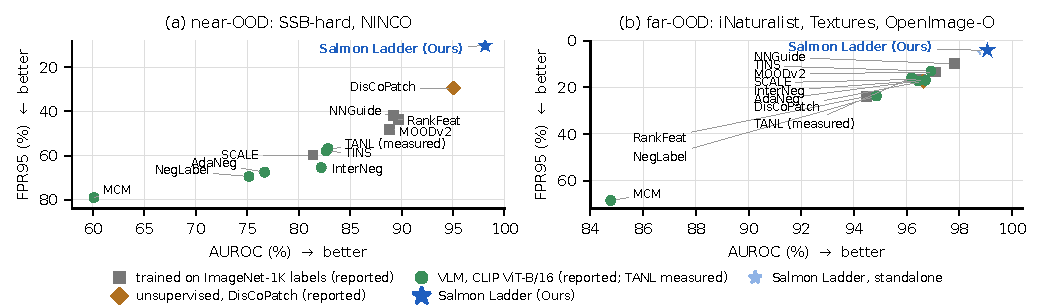
\includegraphics[width=\textwidth]{figs/fig22_scatter.pdf}
\caption{OpenOOD v1.5 ImageNet-1Kでの\AUC{}と\FPR{}（\tabref{main}と\tabref{perds}の比較手法とMCM~\cite{ming2022mcm}，右上ほど良い）．大きな星が本稿の構成（$\sR\times$TINS），小さな星は単体．比較手法は報告値（TANLのみ実測）．}
\label{fig:scatter}
\end{figure*}

\begin{table*}[htbp]
\centering
\caption{Four-OOD（ImageNet-1Kに対するiNaturalist，SUN，Places，Textures，[\%]）．比較手法はすべてCLIP ViT-B/16による報告値$\dagger$（TINSは実測も併記）．記法は\tabref{main}と同じ．}
\label{tab:four}
\vspace{1.5mm}
{\fontsize{7pt}{8.2pt}\selectfont\renewcommand{\arraystretch}{1.0}%
\setlength{\tabcolsep}{2.0pt}\begin{tabular}{@{}lcccccccccc@{}}
\hline
\rule[-2.0pt]{0pt}{8.6pt} & \multicolumn{2}{c}{iNaturalist} & \multicolumn{2}{c}{SUN} & \multicolumn{2}{c}{Places} & \multicolumn{2}{c}{Textures} & \multicolumn{2}{c}{平均} \\
\rule[-2.0pt]{0pt}{8.6pt}手法 & AUROC & FPR95 & AUROC & FPR95 & AUROC & FPR95 & AUROC & FPR95 & AUROC & FPR95 \\
\hline
MCM~\cite{ming2022mcm}$^{\dagger}$ & 94.59 & 32.20 & 92.25 & 38.80 & 90.31 & 46.20 & 86.12 & 58.50 & 90.82 & 43.93 \\
NegLabel~\cite{jiang2024neglabel}$^{\dagger}$ & 99.49 & 1.91 & 95.49 & 20.53 & 91.64 & 35.59 & 90.22 & 43.56 & 94.21 & 25.40 \\
CSP~\cite{chen2024csp}$^{\dagger}$ & 99.60 & 1.54 & 96.66 & 13.66 & 92.90 & 29.32 & 93.86 & 25.52 & 95.76 & 17.51 \\
OODD~\cite{yang2025oodd}$^{\dagger}$ & 99.79 & 0.85 & 97.17 & 12.94 & 92.51 & 30.68 & 94.51 & 30.67 & 96.00 & 18.79 \\
AdaNeg~\cite{zhang2024adaneg}$^{\dagger}$ & 99.71 & 0.59 & 97.44 & 9.50 & 94.55 & 34.34 & 94.93 & 31.27 & 96.66 & 18.92 \\
InterNeg~\cite{xu2026interneg}$^{\dagger}$ & 99.79 & 0.40 & 98.68 & 6.78 & 95.01 & 27.11 & 96.26 & 21.85 & 97.43 & 14.04 \\
TINS~\cite{yang2026tins}$^{\dagger}$ & 99.93 & 0.21 & 99.14 & 3.84 & 97.14 & 12.73 & 97.83 & 10.09 & 98.51 & 6.72 \\
TINS~\cite{yang2026tins}（実測） & 99.93 & 0.22 & 99.12 & 4.35 & 97.12 & 12.98 & 97.94 & 9.83 & 98.52 & 6.85 \\
Salmon Ladder，単体 & 99.93 & \cellcolor{upd}\textbf{0.16} & \cellcolor{upd}\textbf{99.51} & \cellcolor{upd}\textbf{1.64} & 97.06 & \cellcolor{upd}\textbf{11.32} & \cellcolor{upd}\textbf{98.75} & \cellcolor{upd}\textbf{5.07} & \cellcolor{upd}\textbf{98.81} & \cellcolor{upd}\textbf{4.55} \\
{\scriptsize\textcolor{black!60}{\quad 最良の比較手法との差}} & \gap{+0.00} & \gap{+0.05} & \gap{+0.37} & \gap{+2.20} & \gap{-0.08} & \gap{+1.41} & \gap{+0.81} & \gap{+4.76} & \gap{+0.29} & \gap{+2.17} \\
Salmon Ladder $\times$TINS & \cellcolor{upd}\textbf{99.96}\sota & \cellcolor{upd}\textbf{0.11}\sota & \cellcolor{upd}\textbf{99.66}\sota & \cellcolor{upd}\textbf{0.98}\sota & \cellcolor{upd}\textbf{97.56}\sota & \cellcolor{upd}\textbf{9.27}\sota & \cellcolor{upd}\textbf{99.19}\sota & \cellcolor{upd}\textbf{3.17}\sota & \cellcolor{upd}\textbf{99.09}\sota & \cellcolor{upd}\textbf{3.39}\sota \\
{\scriptsize\textcolor{black!60}{\quad 最良の比較手法との差}} & \gap{+0.03} & \gap{+0.10} & \gap{+0.52} & \gap{+2.86} & \gap{+0.42} & \gap{+3.46} & \gap{+1.25} & \gap{+6.66} & \gap{+0.57} & \gap{+3.33} \\
\hline
\end{tabular}}%

\end{table*}

\section{ImageNet-200とCIFAR-100}
\label{sec:app_in200}
\tabref{in200}と\tabref{cifar}に\secref{in200}のImageNet-200とCIFAR-100の値を示す（$\sR$と交差適合した$\sigma$の両方）．$\sR$の$\pfin$の$\alpha{=}0.05$での誤警報率は，ImageNet-200で\NRITNearValFive{}／\NRITFarValFive{}（near／far），CIFAR-100で\NRCFNearValFive{}／\NRCFFarValFive{}である（学習画像の較正）．以下の種と誤警報率の値は$\sigma$のものである．CIFAR-100のIDの誤警報率$\Pr(\pfin\le0.05)$は\NCifarValNearFprZeroZeroFive{}（near）／\NCifarValFarFprZeroZeroFive{}（far），BH法の偽発見割合は\NCifarValNearBhfdp{}／\NCifarValFarBhfdp{}である．CIFAR-100の$32\times32$の画像は他と同じ前処理で拡大して入力し，TexturesはImageNet-1Kベンチマークと同じ画像ファイルなので特徴を共有する．CIFAR-100の種は，Storey型$q{=}0.2$でCIFAR-10・Tiny ImageNetでは折の\NCifarSeedNearStoreyRatioMin{}--\NCifarSeedNearStoreyRatioMax\%，MNIST・SVHN・Places365では\NCifarSeedFarHiStoreyRatioMin{}--\NCifarSeedFarHiStoreyRatioMax\%，Texturesでは\NCifarSeedTextureStoreyRatio\%を占め，種に混じるIDの割合は\NCifarSeedStoreyIdfracMin{}--\NCifarSeedStoreyIdfracMax{}である（DINOv3 L/16のビュー，2つの折・6通りの抽出の平均）．単純BH法の種は折の\NCifarSeedTextureBhRatio{}--\NCifarSeedMnistBhRatio\%，IDの割合\NCifarSeedMnistBhIdfrac{}--\NCifarSeedTinBhIdfrac{}である．種に混じるIDの割合は命題3どおり$q$以下でも，割合$q$の種がIDのほぼ全数になって$\pN$は情報を失う（Places365：$\sigma$ \NCifarMainPlacesThreeSixFiveFpr\%，$\pP$だけ\NCifarLpPlacesThreeSixFiveFpr\%，単純BH法の種で\NCifarBhPlacesThreeSixFiveFpr\%，上限付きの種で\NCifarStoreycPlacesThreeSixFiveFpr\%）．ImageNet-200のSSB-hardでは未知が全画像の\NInTwoZeroZeroMixSsbHard\%を占めてStorey型の$\hat{\pi}_0$が\NInTwoZeroZeroSeedSsbHardStoreyPiZero{}になり，水準$q/\hat{\pi}_0$が1を超えて折の全画像が種になる（単純BH法の種は折の\NInTwoZeroZeroSeedSsbHardBhRatioPct\%，上限付きの種は\NInTwoZeroZeroSeedSsbHardStoreycRatioPct\%，IDの割合\NInTwoZeroZeroSeedSsbHardStoreycIdfrac{}）．

\begin{table}[htbp]
\centering
\caption{OpenOOD v1.5 CIFAR-100（[\%]，単体，\NCifarNDraws{}通りの抽出の平均）．$\dagger$はOpenOOD v1.5~\cite{zhang2023openood}の報告値（\AUC{}は論文の表2，\FPR{}は同論文の脚注6が指す公開の表）．全学習画像のkNN・クラス平均は本稿と同じ2つの特徴（L2正規化して連結），ゼロショットはCLIP ViT-B/16（\secref{in200}）．上限付きの種は$\tau{=}0.05$の$\sigma$（付録\ref{sec:app_cap}）．\textcolor{sotacol}{$\bigstar$}は列の最良値，\colorbox{upd}{青}は本手法以外の全行（報告値，全学習画像・ゼロショットの基線，静的検出器，LGC-max）を上回る値．}
\label{tab:cifar}
\vspace{1.5mm}
{\fontsize{6.8pt}{8pt}\selectfont\renewcommand{\arraystretch}{1.0}%
\setlength{\tabcolsep}{2pt}\begin{tabular}{@{}lcccc@{}}
\hline
\rule[-2.0pt]{0pt}{8.6pt} & \multicolumn{2}{c}{near-OOD} & \multicolumn{2}{c}{far-OOD} \\
\rule[-2.0pt]{0pt}{8.6pt}手法 & AUROC$\uparrow$ & FPR95$\downarrow$ & AUROC$\uparrow$ & FPR95$\downarrow$ \\
\hline
\multicolumn{5}{@{}l}{\rule{0pt}{6.6pt}\textit{CIFAR-100で学習したResNet-18（報告値$^{\dagger}$）}} \\
MSP$^{\dagger}$ & 80.27 & 54.80 & 77.76 & 58.70 \\
MLS$^{\dagger}$ & 81.05 & 55.47 & 79.67 & 56.73 \\
RMDS$^{\dagger}$ & 80.15 & 55.46 & 82.92 & 52.81 \\
VOS$^{\dagger}$ & 80.93 & 55.56 & 81.32 & 53.70 \\
G-ODIN$^{\dagger}$ & 77.15 & 67.58 & 85.67 & 42.68 \\
RotPred$^{\dagger}$ & 76.43 & 62.58 & 88.40 & 34.50 \\
OE$^{\dagger}$（外れ値データで学習） & 88.30 & 30.73 & 81.41 & 54.82 \\
\multicolumn{5}{@{}l}{\rule{0pt}{6.6pt}\textit{全学習画像（50,000枚）またはゼロショット（本稿で実測）}} \\
kNN，全学習画像（$k{=}50$） & 97.09 & 16.35 & 94.94 & 32.15 \\
クラス平均，全学習画像 & 97.61 & 12.91 & 95.38 & 28.05 \\
MCM~\cite{ming2022mcm}，ゼロショット & 70.30 & 94.06 & 74.59 & 89.10 \\
NegLabel~\cite{jiang2024neglabel}，ゼロショット & 72.98 & 76.98 & 80.25 & 64.84 \\
\multicolumn{5}{@{}l}{\rule{0pt}{6.6pt}\textit{凍結特徴，クラスあたり16枚，学習なし，単体（6通りの抽出の平均）}} \\
静的$p$（同じ特徴，グラフなし） & 96.94 & 16.49 & 94.88 & 29.19 \\
kNN（同じ特徴，グラフなし） & 92.35 & 39.22 & 88.47 & 49.80 \\
LGC-max（同じグラフ） & 98.80 & 5.39 & 99.42 & 2.21 \\
$\pP$のみ（種なし，参照画像で読む） & \cellcolor{upd}\textbf{99.11} & \cellcolor{upd}\textbf{2.87} & \cellcolor{upd}\textbf{99.59}\sota & \cellcolor{upd}\textbf{1.17}\sota \\
$\pP\pN$，折も参照画像もなし & \cellcolor{upd}\textbf{99.25} & \cellcolor{upd}\textbf{2.83} & 99.35 & 2.58 \\
$\sigma$（交差適合） & \cellcolor{upd}\textbf{99.18} & \cellcolor{upd}\textbf{2.90} & 99.37 & 2.34 \\
$\sR$（本稿の構成） & \cellcolor{upd}\textbf{99.20} & \cellcolor{upd}\textbf{2.90} & 99.37 & 2.48 \\
$\sigma$，上限付きの種（Storey型） & \cellcolor{upd}\textbf{99.26}\sota & \cellcolor{upd}\textbf{2.55}\sota & \cellcolor{upd}\textbf{99.59} & \cellcolor{upd}\textbf{1.46} \\
$\sigma$，上限付きの種（単純BH法） & \cellcolor{upd}\textbf{99.26}\sota & \cellcolor{upd}\textbf{2.55}\sota & \cellcolor{upd}\textbf{99.59} & \cellcolor{upd}\textbf{1.46} \\
\hline
\end{tabular}}%

\end{table}

\begin{table}[htbp]
\centering
\caption{OpenOOD v1.5 ImageNet-200（[\%]，単体，\NInTwoZeroZeroNDraws{}通りの抽出の平均）．$\dagger$はOpenOOD v1.5~\cite{zhang2023openood}の報告値（ImageNet-200で学習したResNet-18；リーダーボードと同論文の脚注6が指す公開の表）．全学習画像のkNN・クラス平均は本稿と同じ2つの特徴，ゼロショットはCLIP ViT-B/16（\secref{in200}）．上限付きの種は$\tau{=}0.05$の$\sigma$（付録\ref{sec:app_cap}）．\textcolor{sotacol}{$\bigstar$}は列の最良値，\colorbox{upd}{青}は本手法以外の全行（報告値，全学習画像・ゼロショットの基線，静的検出器，LGC-max）を上回る値．}
\label{tab:in200}
\vspace{1.5mm}
{\fontsize{6.8pt}{8pt}\selectfont\renewcommand{\arraystretch}{1.0}%
\setlength{\tabcolsep}{2pt}\begin{tabular}{@{}lcccc@{}}
\hline
\rule[-2.0pt]{0pt}{8.6pt} & \multicolumn{2}{c}{near-OOD} & \multicolumn{2}{c}{far-OOD} \\
\rule[-2.0pt]{0pt}{8.6pt}手法 & AUROC$\uparrow$ & FPR95$\downarrow$ & AUROC$\uparrow$ & FPR95$\downarrow$ \\
\hline
\multicolumn{5}{@{}l}{\rule{0pt}{6.6pt}\textit{ImageNet-200で学習したResNet-18（報告値$^{\dagger}$）}} \\
OE$^{\dagger}$（外れ値データで学習） & 84.84 & 52.30 & 89.02 & 34.17 \\
RegMixup + MSP$^{\dagger}$ & 84.13 & 53.78 & 90.81 & 33.88 \\
TempScale$^{\dagger}$（事後手法の最良） & 83.69 & 54.82 & 90.82 & 34.00 \\
PixMix + ASH$^{\dagger}$ & 81.36 & 63.51 & 95.01 & 21.22 \\
NPOS$^{\dagger}$ & 79.40 & 62.09 & 94.49 & 21.76 \\
\multicolumn{5}{@{}l}{\rule{0pt}{6.6pt}\textit{全学習画像（258,951枚）またはゼロショット（本稿で実測）}} \\
kNN，全学習画像（$k{=}50$） & 92.09 & 28.04 & 98.56 & 4.40 \\
クラス平均，全学習画像 & 92.88 & 24.69 & 98.96 & 3.20 \\
MCM~\cite{ming2022mcm}，ゼロショット & 84.53 & 57.89 & 96.85 & 14.92 \\
NegLabel~\cite{jiang2024neglabel}，ゼロショット & 86.82 & 56.16 & 97.90 & 10.21 \\
\multicolumn{5}{@{}l}{\rule{0pt}{6.6pt}\textit{凍結特徴，クラスあたり16枚，学習なし，単体（6通りの抽出の平均）}} \\
静的$p$（同じ特徴，グラフなし） & 92.25 & 26.72 & 98.71 & 3.71 \\
kNN（同じ特徴，グラフなし） & 89.20 & 38.95 & 97.84 & 7.62 \\
LGC-max（同じグラフ） & 98.31 & 7.99 & 99.41 & 1.65 \\
$\pP$のみ（種なし，参照画像で読む） & \cellcolor{upd}\textbf{98.48}\sota & \cellcolor{upd}\textbf{7.44} & \cellcolor{upd}\textbf{99.42} & \cellcolor{upd}\textbf{1.23}\sota \\
$\pP\pN$，折も参照画像もなし & 98.11 & 9.26 & 99.37 & 2.45 \\
$\sigma$（交差適合） & 98.17 & 9.07 & 99.35 & 2.15 \\
$\sR$（本稿の構成） & 98.22 & 8.68 & 99.40 & 2.06 \\
$\sigma$，上限付きの種（Storey型） & \cellcolor{upd}\textbf{98.43} & \cellcolor{upd}\textbf{6.91}\sota & \cellcolor{upd}\textbf{99.49}\sota & \cellcolor{upd}\textbf{1.23} \\
$\sigma$，上限付きの種（単純BH法） & \cellcolor{upd}\textbf{98.43} & \cellcolor{upd}\textbf{6.91}\sota & \cellcolor{upd}\textbf{99.49}\sota & \cellcolor{upd}\textbf{1.23} \\
\hline
\end{tabular}}%

\end{table}

\section{特徴抽出器の族}
\label{sec:app_views}
本節の値は交差適合した$\sigma$のものである（$\sR$では再計算していない）．\tabref{views}に，ImageNet-1Kのベンチマークで6つの特徴抽出器をそれぞれ単一のビューとして使った値を示す（抽出1通り）．DINOv2 B/14・L/14，DINOv3 B/16・L/16，DINO (v1) ViT-B/16，CLIP ViT-B/16の\NViewsN{}ビューのすべてで，$\sigma$はnear-OODの\FPR{}が静的$p$（\NViewsNMainBelowStaticNear{}/\NViewsN{}），LGC-max（\NViewsNMainBelowLgcNear{}/\NViewsN{}），$\pP$だけ（\NViewsNMainBelowLpNear{}/\NViewsN{}）より低く，交差適合なしの$\pP\pN$との差は\NViewsMinMainMinusVOneNear{}--+\NViewsMaxMainMinusVOneNear{}ポイントである．たとえばCLIP ViT-B/16（ベース検出器と同じ重み）では静的$p$ \NViewClipStaticNearFpr\%から$\sigma$ \NViewClipMainNearFpr\%へ，DINO (v1)では\NViewDinoOneStaticNearFpr\%から\NViewDinoOneMainNearFpr\%へ下がる．利得は自己教師あり学習の世代やVLMかどうかに依らず，特徴空間でIDが支持画像のまわりに集まり未知が互いに近いという性質だけに依る．\textbf{CLIPの静的$p$について．}CLIP ViT-B/16の静的$p$とkNNはnear \NViewClipStaticNearFpr\%，far \NViewClipStaticFarFpr\%とほとんど分離しない．特徴はTINSが使うのと同じ画像埋め込み（投影後，単位ノルム）であり取り違えではなく，同じ特徴でゼロショットのMCMはImageNet-200で動く（\tabref{in200}）．CLIPの画像埋め込みは狭い錐に集まり（支持画像の平均のノルムは\NViewsSupportMeanNormClip{}，DINO系では\NViewsSupportMeanNormDinoMin{}--\NViewsSupportMeanNormDinoMax{}），最も近い原型への余弦はIDで\NViewClipMaxCosIdMean{}$\pm$\NViewClipMaxCosIdStd{}，Texturesで\NViewClipMaxCosOodMean{}$\pm$\NViewClipMaxCosOodStd{}と平均は分かれるが，IDの下側の裾がTexturesの全体を覆うので，IDの95\%を受け入れる閾値ではTexturesのほぼ全部が通る．登録時の仮説「支持画像の平均を引いてから余弦を取れば（中心化）DINO系の範囲に入る」は否定された（付録\ref{sec:app_hyp}）．中心化で静的$p$はnear \NViewClipStaticcNearFpr\%，far \NViewClipStaticcFarFpr\%，kNNはnear \NViewClipKnncNearFpr\%，far \NViewClipKnncFarFpr\%になり，farは\NViewClipCentredMinusRawFarFprAbs{}ポイント改善するがnearはほぼ変わらない（\tabref{views}の中心化の列；DINO系の静的$p$の変化は\NViewsDinoCentredMaxabsFpr{}ポイント以内）．中心化なしの同じ計算（交差適合なし）は表の静的$p$と\NViewsRawVsTableMaxabs{}ポイント以内で一致する．グラフは相対的な近傍だけを使うので，同じ特徴でも$\pP$と$\sigma$はこの影響を受けない．

CLIP ViT-B/16はベース検出器TINSが使う画像エンコーダと同じ重みで，DINO (v1)~\cite{caron2021dino}はImageNet-1Kの画像だけで自己教師あり学習したViT-B/16である．

\begin{table*}[htbp]
\centering
\caption{6つの特徴抽出器をそれぞれ単一のビューとした値（\FPR{}[\%]，OpenOOD v1.5 ImageNet-1K，近＝near-OOD，遠＝far-OOD，抽出1通り）．}
\label{tab:views}
\vspace{1.5mm}
{\fontsize{6.0pt}{7.1pt}\selectfont\renewcommand{\arraystretch}{1.0}%
\setlength{\tabcolsep}{1.3pt}\begin{tabular}{@{}lcc|cc|cc|cc|cc|cc|cc|cc|cc@{}}
\hline
\rule[-2.0pt]{0pt}{8.2pt} & \multicolumn{2}{c|}{静的$p$} & \multicolumn{2}{c|}{静的$p$，中心化} & \multicolumn{2}{c|}{kNN} & \multicolumn{2}{c|}{kNN，中心化} & \multicolumn{2}{c|}{LGC-max} & \multicolumn{2}{c|}{$\pP$のみ} & \multicolumn{2}{c|}{$\pP\pN$（交差なし）} & \multicolumn{2}{c|}{$\sigma$（交差適合）} & \multicolumn{2}{c}{$\sigma\times$TINS} \\
\rule[-2.0pt]{0pt}{8.2pt}ビュー & 近 & 遠 & 近 & 遠 & 近 & 遠 & 近 & 遠 & 近 & 遠 & 近 & 遠 & 近 & 遠 & 近 & 遠 & 近 & 遠 \\
\hline
DINOv2 B/14（768次元） & 61.19 & 21.44 & 62.01 & 22.81 & 65.12 & 23.16 & 65.40 & 24.90 & 28.30 & 13.93 & 16.02 & 8.48 & 15.11 & 6.71 & 15.05 & 6.71 & 14.44 & 5.36 \\
DINOv2 L/14（1024次元） & 55.43 & 20.22 & 55.94 & 21.66 & 59.37 & 25.81 & 59.47 & 27.57 & 24.56 & 13.71 & 14.62 & 8.77 & 14.18 & 7.83 & 14.18 & 7.61 & 13.42 & 5.33 \\
DINOv3 B/16（768次元） & 76.08 & 25.38 & 76.78 & 28.34 & 82.67 & 34.96 & 83.12 & 38.70 & 29.17 & 13.72 & 17.65 & 7.63 & 14.48 & 5.67 & 14.44 & 5.60 & 13.88 & 4.97 \\
DINOv3 L/16（1024次元） & 62.77 & 19.42 & 62.80 & 20.61 & 69.97 & 25.69 & 70.65 & 28.63 & 20.46 & 11.79 & 13.63 & 7.22 & 12.09 & 6.12 & 12.28 & 5.86 & 11.62 & 4.36 \\
DINO (v1) ViT-B/16（768次元） & 80.38 & 40.72 & 83.33 & 49.60 & 86.11 & 52.80 & 88.76 & 63.71 & 46.45 & 19.86 & 30.08 & 10.20 & 27.14 & 8.56 & 26.22 & 8.26 & 24.42 & 7.01 \\
CLIP ViT-B/16（画像埋め込み）（512次元） & 93.64 & 95.38 & 91.41 & 78.46 & 95.91 & 97.41 & 94.65 & 88.81 & 41.12 & 21.53 & 16.67 & 10.38 & 14.20 & 7.14 & 13.43 & 6.60 & 13.79 & 6.07 \\
\hline
\end{tabular}}%

\end{table*}

\section{到着時採点モード}
\label{sec:app_online}
本節のモードは交差適合した$\sigma$で実装した（$\sR$では実行していない）．画像がバッチ（256枚）で順に届く設定では，届いた画像を節点に加えてグラフを厳密な$k_g$近傍グラフに保ち，画像の折は到着番号の偶奇で決める（較正画像の折は最初に1回決める）．各バッチで，$\mathbf{u}^{+}$と各折の$\mathbf{u}^{-}_b$をその時点のグラフ上で\eqnref{lp}の不動点まで反復し（前のバッチの値を初期値にして反復を減らすが，不動点は初期値に依らない．相対残差$10^{-8}$まで平均\NOnlItersMean{}回），種はその時点までに届いた各折の画像に\eqnref{bh}をかけて毎バッチ選び直す．届いたバッチの画像は付録\ref{sec:app_p17}の$\sigma$のとおり採点し，$\pfin$はその時点の自分の折の較正画像の$\sigma$の中での順位で確定して後のバッチで見直さない．到着順がランダムなら，各時点で折$b$の較正画像とそれまでに届いた折$b$のID画像は交換可能なので，命題4と同じ保証が各時点の判定に当てはまる．事後採点との違いは，各画像が「それより後に届く画像」を使えないことだけである．

\tabref{online}に到着時採点モードのデータセット別の値を示す（本稿の2ビュー，Storey型$q{=}0.2$，折は到着番号の偶奇；OpenOODは5通り，Four-OODは3通りの到着順の平均，抽出は1通り）．交差適合なしの到着時採点（v16までの読み出し）も併記する．このモード（near-OODの\FPR{}は単体\NOnlOneFourNoneNearFpr\%，$\times$TINS \NOnlOneFourTinsNearFpr\%）は後に届く画像を使えない分だけ劣るが，報告値の最良は上回る．到着時の$\pfin$のIDの誤警報率$\Pr(\pfin\le0.05)$は近\NOnlOneFourValNearFprZeroZeroFive{}，遠\NOnlOneFourValFarFprZeroZeroFive{}，Four-OOD \NOnlOneFourValFourFprZeroZeroFive{}である（学習画像の較正）．

\begin{table*}[htbp]
\centering
\caption{到着時採点モードのデータセット別の値（[\%]，AUROC／FPR95）．}
\label{tab:online}
\vspace{1.5mm}
{\fontsize{5.8pt}{6.9pt}\selectfont\renewcommand{\arraystretch}{1.0}%
\setlength{\tabcolsep}{0.5pt}\begin{tabular}{@{}lcccccccccccccccccc@{}}
\hline
\rule[-2.0pt]{0pt}{8.6pt} & \multicolumn{2}{c}{SSB-hard} & \multicolumn{2}{c}{NINCO} & \multicolumn{2}{c}{iNat.} & \multicolumn{2}{c}{Textures} & \multicolumn{2}{c}{OImO} & \multicolumn{2}{c}{iNat.} & \multicolumn{2}{c}{SUN} & \multicolumn{2}{c}{Places} & \multicolumn{2}{c}{Textures} \\
\hline
$\sigma\times$TINS & 95.71 & 23.44 & 98.98 & 4.22 & 99.95\sota & 0.09\sota & 99.10\sota & 3.72\sota & 97.56 & 11.94 & 99.95 & 0.12\sota & 99.58\sota & 1.38\sota & 97.40\sota & 10.04\sota & 98.93\sota & 4.44\sota \\
$\sigma$，単体 & 95.48 & 25.44 & 99.05 & 4.15 & 99.91 & 0.18 & 98.64 & 5.59 & 97.24 & 13.12 & 99.91 & 0.21 & 99.42 & 1.92 & 96.88 & 11.76 & 98.41 & 6.63 \\
$\pP\pN\times$TINS，交差適合なし & 95.79\sota & 22.93\sota & 99.04 & 3.85\sota & 99.95 & 0.10 & 99.08 & 4.01 & 97.63\sota & 11.26\sota & 99.95\sota & 0.13 & 99.57 & 1.52 & 97.38 & 10.14 & 98.92 & 4.60 \\
$\pP\pN$，単体，交差適合なし & 95.49 & 25.32 & 99.08\sota & 3.87 & 99.92 & 0.20 & 98.61 & 6.13 & 97.30 & 12.61 & 99.91 & 0.22 & 99.41 & 2.27 & 96.85 & 12.27 & 98.39 & 7.07 \\
\hline
\end{tabular}}%

\end{table*}

\section{開発用分割での構成の選択}
\label{sec:app_sel}
\tabref{sel}に第1段（ビューと$q$，交差適合なしの$\pP\pN$），\tabref{selq}に第2段（交差適合の種の規則・$q$・統計量）の，開発用分割dev1（選択）とdev2（確認）での候補の値を示す（単体，5通りの抽出の平均；各分割はnearとfarの2つの未知の集合を持つ）．第2段では，静的$p$を統計量に含める候補はdev1のfar-OODでは最も良いがnear-OODで悪く（\NSelqDevOnePpsNearFpr\%／\NSelqDevOnePpsFarFpr\%），$q{=}0.05$はどの組でも悪い．選ばれたStorey型・$q{=}0.2$・$\pP\pN$はdev1 nearで\NSelqDevOneNearFpr\%（\NSelqNCandidates{}候補中\NSelqDevOneRankOfChosen{}位），dev2 nearで\NSelqDevTwoNearFpr\%であり，交差適合なしの参照（dev1 \NSelqRefDevOneNearFpr\%）より良い．LGC-maxはdev1 nearで\NSelqDevOneLgcNearFpr\%である．$\sR$はこの選択の後に，選ばれた$\sigma$の折を参照画像に置き換えるものとして登録した（付録\ref{sec:app_p17}）．

\begin{table*}[htbp]
\centering
\caption{第1段の候補（ビューと$q$；[\%]，交差適合なしの$\pP\pN$，単体，5通りの抽出の平均）．\textcolor{sotacol}{$\bigstar$}は列の最良値．}
\label{tab:sel}
\vspace{1.5mm}
{\fontsize{6.6pt}{7.8pt}\selectfont\renewcommand{\arraystretch}{1.0}%
\setlength{\tabcolsep}{2.0pt}\begin{tabular}{@{}lcccccccc@{}}
\hline
\rule[-2.0pt]{0pt}{8.6pt} & \multicolumn{4}{c}{dev1（選択）} & \multicolumn{4}{c}{dev2（確認）} \\
\rule[-2.0pt]{0pt}{8.6pt} & \multicolumn{2}{c}{near} & \multicolumn{2}{c}{far} & \multicolumn{2}{c}{near} & \multicolumn{2}{c}{far} \\
\rule[-2.0pt]{0pt}{8.6pt}構成（$\pP\pN$，単体） & AUROC & FPR95 & AUROC & FPR95 & AUROC & FPR95 & AUROC & FPR95 \\
\hline
DINOv2 L/14，$q{=}0.05$ & 94.95 & 21.50 & 95.29 & 22.03 & 94.84 & 22.59 & 95.18 & 23.19 \\
DINOv2 L/14，$q{=}0.1$ & 95.69 & 18.43 & 95.36 & 22.19 & 95.66 & 18.40 & 95.35 & 22.34 \\
DINOv2 L/14，$q{=}0.2$ & 95.94 & 19.26 & 95.68 & 20.12 & 96.11 & 18.12 & 95.56 & 20.92 \\
DINOv3 L/16，$q{=}0.05$ & 95.69 & 20.80 & 95.59 & 20.54 & 95.86 & 18.71 & 95.55 & 20.00 \\
DINOv3 L/16，$q{=}0.1$ & 96.57 & 16.38 & 95.87 & 19.57 & 96.73 & 15.52 & 95.85 & 18.62 \\
DINOv3 L/16，$q{=}0.2$ & 96.81 & 16.86 & 96.28 & 17.19 & 96.94 & 15.65 & 96.12 & 17.40 \\
連結ビュー，$q{=}0.05$ & 96.03 & 17.23 & 95.96 & 19.49 & 95.95 & 17.82 & 95.92 & 19.75 \\
連結ビュー，$q{=}0.1$ & 96.66 & 15.34 & 96.09 & 18.94 & 96.57 & 14.62 & 96.11 & 18.87 \\
連結ビュー，$q{=}0.2$ & 96.79 & 15.86 & 96.45 & 16.91 & 96.86 & 14.48 & 96.37 & 17.47 \\
DINOv2 L/14 + DINOv3 L/16，$q{=}0.05$ & 96.34 & 17.15 & 96.36 & 17.84 & 96.25 & 17.27 & 96.32 & 17.73 \\
DINOv2 L/14 + DINOv3 L/16，$q{=}0.1$ & 96.89 & 14.59 & 96.40 & 18.05 & 96.91 & 14.35 & 96.39 & 17.60 \\
DINOv2 L/14 + DINOv3 L/16，$q{=}0.2$（選択） & 97.06 & 14.10\sota & 96.71 & 16.43 & 97.16 & 13.58 & 96.57 & 16.93 \\
連結ビュー + DINOv3 L/16，$q{=}0.05$ & 96.39 & 17.17 & 96.17 & 18.03 & 96.35 & 16.46 & 96.09 & 18.49 \\
連結ビュー + DINOv3 L/16，$q{=}0.1$ & 96.96 & 14.44 & 96.30 & 17.96 & 96.98 & 13.91 & 96.30 & 17.42 \\
連結ビュー + DINOv3 L/16，$q{=}0.2$ & 97.10\sota & 14.37 & 96.68 & 16.39\sota & 97.18\sota & 13.53\sota & 96.54 & 16.78 \\
DINOv3 B/16 + L/16，$q{=}0.05$ & 94.73 & 24.54 & 95.62 & 20.93 & 94.94 & 22.85 & 95.58 & 20.15 \\
DINOv3 B/16 + L/16，$q{=}0.1$ & 95.92 & 20.30 & 95.96 & 19.30 & 96.03 & 19.12 & 95.89 & 18.89 \\
DINOv3 B/16 + L/16，$q{=}0.2$ & 96.33 & 19.13 & 96.37 & 17.95 & 96.41 & 18.50 & 96.19 & 17.47 \\
DINOv2 B/14 + L/14，$q{=}0.05$ & 94.80 & 23.72 & 95.73 & 21.20 & 94.62 & 23.77 & 95.72 & 21.01 \\
DINOv2 B/14 + L/14，$q{=}0.1$ & 95.73 & 19.74 & 95.85 & 20.61 & 95.59 & 19.34 & 95.73 & 20.75 \\
DINOv2 B/14 + L/14，$q{=}0.2$ & 96.03 & 19.06 & 96.15 & 19.08 & 96.11 & 18.11 & 95.98 & 19.77 \\
DINOv2 L/14 + DINOv3 B/16 + L/16，$q{=}0.05$ & 95.95 & 19.30 & 96.30 & 18.30 & 95.72 & 19.52 & 96.27 & 18.01 \\
DINOv2 L/14 + DINOv3 B/16 + L/16，$q{=}0.1$ & 96.64 & 16.11 & 96.40 & 18.18 & 96.54 & 16.38 & 96.36 & 17.48 \\
DINOv2 L/14 + DINOv3 B/16 + L/16，$q{=}0.2$ & 96.87 & 15.52 & 96.74\sota & 16.51 & 96.89 & 15.50 & 96.59\sota & 16.46\sota \\
\hline
\end{tabular}}%

\end{table*}

\begin{table*}[htbp]
\centering
\caption{第2段の候補（交差適合の種の規則・$q$・統計量；[\%]，$\pfin$，単体，5通りの抽出の平均，折は3通りの割り当ての平均）と参照．\textcolor{sotacol}{$\bigstar$}は列の最良値．}
\label{tab:selq}
\vspace{1.5mm}
{\fontsize{6.6pt}{7.8pt}\selectfont\renewcommand{\arraystretch}{1.0}%
\setlength{\tabcolsep}{2.0pt}\begin{tabular}{@{}lcccccccc@{}}
\hline
\rule[-2.0pt]{0pt}{8.6pt} & \multicolumn{4}{c}{dev1（選択）} & \multicolumn{4}{c}{dev2（確認）} \\
\rule[-2.0pt]{0pt}{8.6pt} & \multicolumn{2}{c}{near} & \multicolumn{2}{c}{far} & \multicolumn{2}{c}{near} & \multicolumn{2}{c}{far} \\
\rule[-2.0pt]{0pt}{8.6pt}候補（$\pfin$，単体） & AUROC & FPR95 & AUROC & FPR95 & AUROC & FPR95 & AUROC & FPR95 \\
\hline
Storey型，$q{=}0.2$，$\pP\pN$（選択） & 97.08 & 13.55 & 96.66 & 16.53 & 97.15 & 13.01\sota & 96.54 & 16.97 \\
Storey型，$q{=}0.2$，$\pP\pN\times$静的$p$ & 96.68 & 16.29 & 97.67\sota & 11.33\sota & 96.73 & 15.28 & 97.60\sota & 11.50\sota \\
Storey型，$q{=}0.2$，$\min(\pP\pN,$静的$p)$ & 97.09 & 13.74 & 96.93 & 15.58 & 97.16 & 13.14 & 96.80 & 16.03 \\
Storey型，$q{=}0.1$，$\pP\pN$ & 96.84 & 14.59 & 96.48 & 17.39 & 96.84 & 14.39 & 96.36 & 17.69 \\
Storey型，$q{=}0.1$，$\pP\pN\times$静的$p$ & 96.41 & 17.48 & 97.59 & 11.56 & 96.39 & 16.48 & 97.52 & 11.72 \\
Storey型，$q{=}0.1$，$\min(\pP\pN,$静的$p)$ & 96.87 & 14.73 & 96.82 & 15.95 & 96.85 & 14.52 & 96.69 & 16.33 \\
Storey型，$q{=}0.05$，$\pP\pN$ & 96.23 & 17.74 & 96.40 & 17.47 & 96.08 & 18.16 & 96.38 & 17.36 \\
Storey型，$q{=}0.05$，$\pP\pN\times$静的$p$ & 95.71 & 20.92 & 97.52 & 11.92 & 95.62 & 19.67 & 97.50 & 11.81 \\
Storey型，$q{=}0.05$，$\min(\pP\pN,$静的$p)$ & 96.25 & 17.98 & 96.93 & 15.30 & 96.08 & 18.24 & 96.90 & 15.08 \\
単純BH，$q{=}0.2$，$\pP\pN$ & 97.03 & 13.77 & 96.64 & 16.65 & 97.07 & 13.37 & 96.52 & 16.99 \\
単純BH，$q{=}0.2$，$\pP\pN\times$静的$p$ & 96.62 & 16.55 & 97.66 & 11.36 & 96.63 & 15.62 & 97.59 & 11.53 \\
単純BH，$q{=}0.2$，$\min(\pP\pN,$静的$p)$ & 97.04 & 14.00 & 96.91 & 15.73 & 97.07 & 13.51 & 96.80 & 16.10 \\
単純BH，$q{=}0.1$，$\pP\pN$ & 96.72 & 15.19 & 96.45 & 17.52 & 96.65 & 15.30 & 96.35 & 17.72 \\
単純BH，$q{=}0.1$，$\pP\pN\times$静的$p$ & 96.27 & 18.01 & 97.57 & 11.72 & 96.19 & 17.19 & 97.52 & 11.74 \\
単純BH，$q{=}0.1$，$\min(\pP\pN,$静的$p)$ & 96.75 & 15.36 & 96.80 & 16.09 & 96.66 & 15.43 & 96.68 & 16.45 \\
単純BH，$q{=}0.05$，$\pP\pN$ & 95.89 & 19.70 & 96.43 & 17.13 & 95.72 & 19.95 & 96.40 & 17.28 \\
単純BH，$q{=}0.05$，$\pP\pN\times$静的$p$ & 95.32 & 22.93 & 97.53 & 11.88 & 95.28 & 21.25 & 97.50 & 11.84 \\
単純BH，$q{=}0.05$，$\min(\pP\pN,$静的$p)$ & 95.90 & 19.97 & 97.00 & 14.77 & 95.72 & 19.97 & 96.94 & 14.90 \\
参照：$\pP\pN$，交差適合なし（Storey型，$q{=}0.2$） & 97.06 & 14.10 & 96.71 & 16.43 & 97.16 & 13.58 & 96.57 & 16.93 \\
$\pP$のみ & 95.65 & 18.81 & 96.50 & 16.46 & 95.99 & 17.40 & 96.44 & 17.14 \\
静的$p$ & 84.84 & 58.45 & 97.12 & 13.30 & 85.36 & 57.77 & 97.19 & 13.16 \\
kNN & 80.13 & 68.20 & 96.00 & 19.05 & 79.42 & 66.82 & 95.95 & 19.08 \\
LGC-max & 91.80 & 38.05 & 94.04 & 29.53 & 93.24 & 32.97 & 94.32 & 28.38 \\
選択した構成の$\sigma$（順位付けの統計量） & 97.10\sota & 13.54\sota & 96.67 & 16.60 & 97.17\sota & 13.09 & 96.54 & 17.00 \\
選択した構成の$\sigma\times$TINS & 97.09 & 13.80 & 96.85 & 15.94 & 97.12 & 13.44 & 96.71 & 16.44 \\
選択した構成の$\pfin\times$TINS & 96.82 & 14.99 & 96.73 & 16.71 & 96.74 & 15.07 & 96.52 & 17.87 \\
\hline
\end{tabular}}%

\end{table*}

\section{テスト集合での感度と選択の履歴}
\label{sec:app_sens}
\tabref{ablx}に，\tabref{abl}の読み出しの単体での値と，$\sigma$の第2段の候補（種の規則，$q$，統計量）の一部のテスト集合での値を示す．テスト集合では単純BH法の種がStorey型よりわずかに良く，$q{=}0.1$が$q{=}0.2$よりわずかに良いが，構成は開発用分割の規則で選んだものを変えない（\secref{exp}，付録\ref{sec:app_devtest}）．\tabref{sens}に，交差適合なしの$\pP\pN$について，ビューの組と$q$とベース検出器のすべての組合せのテスト集合での値（6通りの抽出の平均）を示す．v16までの版では，グラフの近傍数，相互近傍グラフ，$\lambda$，種の2巡目，種への最近傍項，重み，DINOv3の採用，静的$p$との積をテスト集合上で探索し，その上で第1段の候補の集合を決めた．本稿の構成はこの表からは選んでおらず（\secref{exp}），交差適合に関わる第2段の候補と規則，$\sR$とその採否の規則はテスト集合の計算前に登録した．探索の記録は\url{https://github.com/omotes24/SalmonLadder}に残している．

\begin{table*}[htbp]
\centering
\caption{同じ特徴での読み出しの比較（単体）と$\sigma$の第2段の他の候補の値（[\%]，6通りの抽出の平均）．記法は\tabref{abl}と同じ．}
\label{tab:ablx}
\vspace{1.5mm}
{\fontsize{6.8pt}{8.0pt}\selectfont\renewcommand{\arraystretch}{1.0}%
\setlength{\tabcolsep}{2.0pt}\begin{tabular}{@{}lcccccc@{}}
\hline
\rule[-2.0pt]{0pt}{8.6pt} & \multicolumn{2}{c}{OpenOOD near-OOD} & \multicolumn{2}{c}{OpenOOD far-OOD} & \multicolumn{2}{c}{Four-OOD} \\
\rule[-2.0pt]{0pt}{8.6pt}構成 & AUROC$\uparrow$ & FPR95$\downarrow$ & AUROC$\uparrow$ & FPR95$\downarrow$ & AUROC$\uparrow$ & FPR95$\downarrow$ \\
\hline
\multicolumn{7}{@{}l}{\rule{0pt}{6.6pt}\textit{同じ特徴での読み出し，単体}} \\
静的$p$ & 82.30 & 54.36 & 96.48 & 15.92 & 93.77 & 24.85 \\
kNN~\cite{sun2022knn} & 78.75 & 59.51 & 95.52 & 19.27 & 92.71 & 28.55 \\
LGC-max & 95.69 & 19.52 & 97.70 & 10.13 & 96.98 & 11.38 \\
$\pP$のみ & 97.54 & 12.36 & 98.46 & 6.04 & 98.26 & 5.73 \\
$\pP\pN$，折も参照画像もなし & 97.96 & 11.39 & 98.80 & 5.21 & 98.79 & 4.69 \\
$\sigma$：2つの折で交差適合した$\pP\pN$ & 97.94 & 11.50 & 98.79 & 5.17 & 98.80 & 4.56 \\
$\sigma$，上限付きの種（Storey型） & 97.78 & 11.32 & 98.83 & 5.00 & 98.80 & 4.54 \\
$\sigma$，上限付きの種（単純BH法） & 97.79 & 11.29 & 98.84 & 4.94 & 98.83 & 4.43 \\
$\sR$：参照画像で種を選び読む$\pP\pN$ & 97.98 & 11.26 & 98.81 & 5.14 & 98.81 & 4.55 \\
$\sR$の較正順位$\pfin$をそのままスコアにしたもの & 97.97 & 11.26 & 98.79 & 5.14 & 98.80 & 4.55 \\
$\pP\pN$，到着時採点，折なし & 97.28 & 14.60 & 98.61 & 6.31 & 98.64 & 5.46 \\
$\sigma$，到着時採点 & 97.26 & 14.80 & 98.60 & 6.29 & 98.65 & 5.13 \\
\multicolumn{7}{@{}l}{\rule{0pt}{6.6pt}\textit{$\sigma$の第2段の他の候補（\tabref{selq}），$\times$TINS}} \\
$\sigma$（Storey型，$q{=}0.2$） & 98.09\sota & 10.50 & 99.05 & 4.16 & 99.09 & 3.39 \\
$\sigma$，種を単純BH法で選択 & 98.03 & 10.29 & 99.07 & 4.03 & 99.10 & 3.32 \\
$\sigma$に静的$p$を加える & 97.72 & 12.16 & 99.19 & 3.69 & 99.00 & 3.75 \\
$\min(\sigma,\,\log$静的$p)$ & 98.06 & 10.54 & 99.08 & 4.14 & 99.09 & 3.36 \\
単純BH法の種，静的$p$を加える & 97.63 & 11.94 & 99.20\sota & 3.64\sota & 99.01 & 3.72 \\
$\sigma$，$q{=}0.1$ & 98.06 & 10.26 & 99.09 & 3.96 & 99.12\sota & 3.20 \\
$\sigma$，$q{=}0.05$ & 97.87 & 10.74 & 99.08 & 4.03 & 99.11 & 3.07\sota \\
単純BH法の種，$q{=}0.1$ & 97.84 & 10.82 & 99.10 & 3.95 & 99.12 & 3.15 \\
$\pP\pN$，折なし，$q{=}0.1$ & 98.08 & 10.08\sota & 99.09 & 4.00 & 99.11 & 3.25 \\
$\pP\pN$，折なし，$q{=}0.05$ & 97.88 & 10.64 & 99.09 & 4.00 & 99.11 & 3.09 \\
\hline
\end{tabular}}%

\end{table*}

\begin{table*}[htbp]
\centering
\caption{テスト集合での感度（[\%]，交差適合なしの$\pP\pN$，6通りの抽出の平均）．\textcolor{sotacol}{$\bigstar$}は列の最良値．}
\label{tab:sens}
\vspace{1.5mm}
{\fontsize{7pt}{8.2pt}\selectfont\renewcommand{\arraystretch}{1.0}%
\setlength{\tabcolsep}{2.2pt}\begin{tabular}{@{}lcccccc@{}}
\hline
\rule[-2.0pt]{0pt}{8.6pt} & \multicolumn{2}{c}{OpenOOD near-OOD} & \multicolumn{2}{c}{OpenOOD far-OOD} & \multicolumn{2}{c}{Four-OOD} \\
\rule[-2.0pt]{0pt}{8.6pt}構成（交差適合なしの$\pP\pN$） & AUROC$\uparrow$ & FPR95$\downarrow$ & AUROC$\uparrow$ & FPR95$\downarrow$ & AUROC$\uparrow$ & FPR95$\downarrow$ \\
\hline
DINOv2 L/14，$q{=}0.05$，単体 & 97.36 & 13.01 & 98.54 & 6.04 & 98.53 & 5.28 \\
DINOv2 L/14，$q{=}0.05$，$\times$TINS & 97.43 & 12.40 & 98.93 & 4.80 & 99.04 & 3.43 \\
DINOv2 L/14，$q{=}0.1$，単体 & 97.54 & 12.81 & 98.50 & 6.43 & 98.50 & 5.74 \\
DINOv2 L/14，$q{=}0.1$，$\times$TINS & 97.64 & 11.98 & 98.94 & 4.78 & 99.04 & 3.64 \\
DINOv2 L/14，$q{=}0.2$，単体 & 97.47 & 13.69 & 98.38 & 7.02 & 98.37 & 6.52 \\
DINOv2 L/14，$q{=}0.2$，$\times$TINS & 97.64 & 12.55 & 98.89 & 4.98 & 99.00 & 3.94 \\
DINOv3 L/16，$q{=}0.05$，単体 & 97.72 & 11.69 & 98.79 & 4.91 & 98.83 & 4.04 \\
DINOv3 L/16，$q{=}0.05$，$\times$TINS & 97.72 & 11.31 & 99.05 & 4.11 & 99.15 & 2.90\sota \\
DINOv3 L/16，$q{=}0.1$，単体 & 97.91 & 11.06 & 98.79 & 5.17 & 98.83 & 4.33 \\
DINOv3 L/16，$q{=}0.1$，$\times$TINS & 97.93 & 10.56 & 99.07 & 4.02 & 99.17\sota & 3.00 \\
DINOv3 L/16，$q{=}0.2$，単体 & 97.91 & 11.62 & 98.71 & 5.55 & 98.75 & 4.88 \\
DINOv3 L/16，$q{=}0.2$，$\times$TINS & 97.97 & 10.81 & 99.04 & 4.18 & 99.14 & 3.19 \\
連結ビュー，$q{=}0.05$，単体 & 97.75 & 11.34 & 98.78 & 4.88 & 98.76 & 4.36 \\
連結ビュー，$q{=}0.05$，$\times$TINS & 97.76 & 11.06 & 99.05 & 4.10 & 99.12 & 3.07 \\
連結ビュー，$q{=}0.1$，単体 & 97.90 & 11.08 & 98.75 & 5.27 & 98.74 & 4.71 \\
連結ビュー，$q{=}0.1$，$\times$TINS & 97.93 & 10.59 & 99.06 & 4.08 & 99.12 & 3.21 \\
連結ビュー，$q{=}0.2$，単体 & 97.83 & 11.90 & 98.65 & 5.74 & 98.64 & 5.39 \\
連結ビュー，$q{=}0.2$，$\times$TINS & 97.93 & 11.10 & 99.02 & 4.29 & 99.09 & 3.46 \\
DINOv2 L/14 + DINOv3 L/16，$q{=}0.05$，単体 & 97.79 & 11.28 & 98.90 & 4.71 & 98.89 & 3.96 \\
DINOv2 L/14 + DINOv3 L/16，$q{=}0.05$，$\times$TINS & 97.88 & 10.64 & 99.09 & 4.00 & 99.11 & 3.09 \\
DINOv2 L/14 + DINOv3 L/16，$q{=}0.1$，単体 & 97.97 & 10.87 & 98.88 & 4.84 & 98.88 & 4.23 \\
DINOv2 L/14 + DINOv3 L/16，$q{=}0.1$，$\times$TINS & 98.08 & 10.08 & 99.09\sota & 4.00 & 99.11 & 3.25 \\
DINOv2 L/14 + DINOv3 L/16，$q{=}0.2$，単体 & 97.96 & 11.39 & 98.80 & 5.21 & 98.79 & 4.69 \\
DINOv2 L/14 + DINOv3 L/16，$q{=}0.2$，$\times$TINS & 98.12 & 10.26 & 99.05 & 4.21 & 99.07 & 3.50 \\
連結ビュー + DINOv3 L/16，$q{=}0.05$，単体 & 97.84 & 11.15 & 98.88 & 4.61 & 98.88 & 3.93 \\
連結ビュー + DINOv3 L/16，$q{=}0.05$，$\times$TINS & 97.93 & 10.45 & 99.08 & 3.91\sota & 99.10 & 3.06 \\
連結ビュー + DINOv3 L/16，$q{=}0.1$，単体 & 98.00 & 10.65 & 98.87 & 4.83 & 98.87 & 4.22 \\
連結ビュー + DINOv3 L/16，$q{=}0.1$，$\times$TINS & 98.12 & 9.87\sota & 99.08 & 4.02 & 99.11 & 3.23 \\
連結ビュー + DINOv3 L/16，$q{=}0.2$，単体 & 97.97 & 11.24 & 98.78 & 5.18 & 98.78 & 4.71 \\
連結ビュー + DINOv3 L/16，$q{=}0.2$，$\times$TINS & 98.14\sota & 10.10 & 99.03 & 4.23 & 99.07 & 3.57 \\
\hline
\end{tabular}}%

\end{table*}

\section{再出現と混入率の格子}
\label{sec:app_rec}
\tabref{recrefninco}と\tabref{recrefssb}に，\secref{rec}の格子の全条件での$\sR$の値を，静的$p$，$\pP$だけ（参照画像で読む），交差適合した$\sigma$と並べて示す（\FPR{}，単体と$\times$TINS，3回の平均；種は$\sR$のDINOv3 L/16のビューで選ばれた枚数とそのうちIDの割合（\%））．\tabref{recninco}と\tabref{recssb}は交差適合した$\sigma$の詳細（v18--v21の表）である．$\sigma$と交差適合なしの$\pP\pN$との\FPR{}の差は\NRecNAll{}条件で\NRecMinMainMinusVOne{}--+\NRecMaxMainMinusVOne{}ポイントの範囲にある．$\sigma$に静的$p$を加えると，$r\le5$で静的$p$に劣る条件は\NRecNRLeFivePpsWorseStatic{}に減り差も最大\NRecMaxPpsMinusStaticLeFive{}ポイントになるが，64クラス$\times$30枚では\NRecNincoCSixFourRThreeZeroMainFpr\%から\NRecNincoCSixFourRThreeZeroPpsFpr\%へ悪化する．$c$は未知クラスの数，$r$は各クラスの枚数，混入率は未知の枚数をテスト集合の枚数で割った値．$\sigma$の表の検出器の列は\AUC{}／\FPR{}（DINOv2 L/14 + DINOv3 L/16，ラベル付き画像は本稿の抽出1通り，クラスと画像の選び方を変えた3回の平均；学習画像の較正）．$\Pr(\pfin\le0.05)$は$\sigma$の$\pfin$のIDの誤警報率．種はDINOv3 L/16のビューでStorey型$q{=}0.2$のときに選ばれた枚数（2つの折の合計），IDはそのうちIDだった割合（\%），再現は未知のうち種に選ばれた割合（\%）．

\begin{table}[htbp]
\centering
\caption{再出現と混入率の格子：NINCO，$\sR$（\FPR{}[\%]）．}
\label{tab:recrefninco}
\vspace{1.5mm}
{\fontsize{6.2pt}{7.2pt}\selectfont\renewcommand{\arraystretch}{1.0}%
\setlength{\tabcolsep}{2.6pt}\begin{tabular}{@{}rrrr|ccccc|rr@{}}
\hline
\rule[-2.0pt]{0pt}{8.2pt}$c$ & $r$ & 未知 & 混入率 & 静的$p$ & $\pP$（参照） & $\sigma$ & $\sR$ & $\sR\times$TINS & 種 & ID \\
\hline
5 & 1 & 5 & 0.01 & 33.3 & 73.3 & 73.3 & 73.3 & 46.7 & 0 & -- \\
5 & 2 & 10 & 0.02 & 63.3 & 76.7 & 76.7 & 76.7 & 53.3 & 0 & -- \\
5 & 5 & 25 & 0.06 & 46.7 & 74.7 & 76.0 & 74.7 & 62.7 & 0 & -- \\
5 & 10 & 50 & 0.11 & 69.3 & 41.3 & 40.7 & 41.3 & 39.3 & 0 & -- \\
5 & 20 & 100 & 0.22 & 43.3 & 10.7 & 11.7 & 10.7 & 12.3 & 0 & -- \\
5 & 30 & 150 & 0.33 & 34.2 & 14.7 & 10.9 & 14.7 & 8.7 & 73 & 40 \\
10 & 1 & 10 & 0.02 & 33.3 & 73.3 & 73.3 & 73.3 & 60.0 & 0 & -- \\
10 & 2 & 20 & 0.04 & 55.0 & 78.3 & 78.3 & 78.3 & 51.7 & 0 & -- \\
10 & 5 & 50 & 0.11 & 52.7 & 70.7 & 70.7 & 70.7 & 55.3 & 0 & -- \\
10 & 10 & 100 & 0.22 & 45.7 & 26.7 & 28.7 & 26.7 & 25.3 & 0 & -- \\
10 & 20 & 200 & 0.44 & 39.2 & 10.8 & 8.8 & 9.7 & 8.3 & 76 & 39 \\
10 & 30 & 300 & 0.66 & 35.1 & 4.9 & 1.4 & 2.6 & 3.1 & 338 & 51 \\
20 & 1 & 20 & 0.04 & 35.0 & 60.0 & 60.0 & 60.0 & 45.0 & 0 & -- \\
20 & 2 & 40 & 0.09 & 40.0 & 78.3 & 77.5 & 78.3 & 58.3 & 0 & -- \\
20 & 5 & 100 & 0.22 & 45.7 & 68.0 & 68.0 & 68.0 & 49.7 & 0 & -- \\
20 & 10 & 200 & 0.44 & 44.5 & 34.8 & 36.2 & 34.8 & 30.8 & 0 & -- \\
20 & 20 & 400 & 0.88 & 52.5 & 11.8 & 9.0 & 8.5 & 7.7 & 308 & 45 \\
20 & 30 & 600 & 1.32 & 45.6 & 7.0 & 3.9 & 3.8 & 2.2 & 989 & 46 \\
40 & 1 & 40 & 0.09 & 47.5 & 75.8 & 75.8 & 75.8 & 55.8 & 0 & -- \\
40 & 2 & 80 & 0.18 & 46.2 & 70.0 & 70.8 & 70.0 & 52.9 & 0 & -- \\
40 & 5 & 200 & 0.44 & 46.5 & 68.2 & 67.8 & 68.2 & 49.3 & 0 & -- \\
40 & 10 & 400 & 0.88 & 48.9 & 34.8 & 35.2 & 35.2 & 30.0 & 35 & 42 \\
40 & 20 & 800 & 1.75 & 49.8 & 12.9 & 9.8 & 8.2 & 7.8 & 1,029 & 44 \\
40 & 30 & 1,200 & 2.60 & 45.1 & 5.8 & 2.7 & 3.2 & 2.6 & 1,856 & 44 \\
64 & 1 & 64 & 0.14 & 44.3 & 75.0 & 75.0 & 75.0 & 57.8 & 0 & -- \\
64 & 2 & 128 & 0.28 & 46.1 & 72.1 & 72.4 & 72.1 & 54.9 & 0 & -- \\
64 & 5 & 320 & 0.71 & 46.2 & 61.5 & 60.9 & 61.5 & 47.8 & 0 & -- \\
64 & 10 & 640 & 1.40 & 46.9 & 33.6 & 30.2 & 31.0 & 28.1 & 119 & 37 \\
64 & 20 & 1,280 & 2.77 & 45.5 & 11.9 & 7.9 & 7.7 & 6.7 & 1,675 & 41 \\
64 & 30 & 1,920 & 4.09 & 46.0 & 6.8 & 2.5 & 3.0 & 2.3 & 2,839 & 40 \\
\hline
\end{tabular}}%

\end{table}

\begin{table}[htbp]
\centering
\caption{再出現と混入率の格子：SSB-hard，$\sR$（\FPR{}[\%]）．}
\label{tab:recrefssb}
\vspace{1.5mm}
{\fontsize{6.2pt}{7.2pt}\selectfont\renewcommand{\arraystretch}{1.0}%
\setlength{\tabcolsep}{2.6pt}\begin{tabular}{@{}rrrr|ccccc|rr@{}}
\hline
\rule[-2.0pt]{0pt}{8.2pt}$c$ & $r$ & 未知 & 混入率 & 静的$p$ & $\pP$（参照） & $\sigma$ & $\sR$ & $\sR\times$TINS & 種 & ID \\
\hline
10 & 1 & 10 & 0.02 & 66.7 & 90.0 & 90.0 & 90.0 & 60.0 & 0 & -- \\
10 & 2 & 20 & 0.04 & 73.3 & 86.7 & 86.7 & 86.7 & 66.7 & 0 & -- \\
10 & 5 & 50 & 0.11 & 53.3 & 82.0 & 82.0 & 82.0 & 52.7 & 0 & -- \\
10 & 10 & 100 & 0.22 & 63.3 & 60.3 & 60.0 & 60.3 & 46.0 & 0 & -- \\
10 & 20 & 200 & 0.44 & 69.8 & 46.8 & 45.8 & 46.8 & 40.3 & 0 & -- \\
10 & 50 & 500 & 1.10 & 65.7 & 18.3 & 11.5 & 11.6 & 10.5 & 422 & 39 \\
30 & 1 & 30 & 0.07 & 55.6 & 71.1 & 71.1 & 71.1 & 50.0 & 0 & -- \\
30 & 2 & 60 & 0.13 & 65.0 & 83.9 & 82.8 & 83.9 & 63.3 & 0 & -- \\
30 & 5 & 150 & 0.33 & 65.1 & 78.9 & 79.1 & 78.9 & 67.3 & 0 & -- \\
30 & 10 & 300 & 0.66 & 58.9 & 60.4 & 60.7 & 60.4 & 48.4 & 0 & -- \\
30 & 20 & 600 & 1.32 & 71.0 & 46.2 & 43.3 & 46.1 & 40.4 & 154 & 31 \\
30 & 50 & 1,500 & 3.23 & 67.3 & 25.2 & 16.5 & 16.8 & 14.1 & 1,622 & 44 \\
100 & 1 & 100 & 0.22 & 65.0 & 79.7 & 80.0 & 79.7 & 62.0 & 0 & -- \\
100 & 2 & 200 & 0.44 & 71.0 & 83.8 & 84.0 & 83.8 & 66.3 & 0 & -- \\
100 & 5 & 500 & 1.10 & 70.3 & 76.4 & 76.1 & 76.4 & 59.5 & 0 & -- \\
100 & 10 & 1,000 & 2.17 & 68.1 & 56.4 & 50.7 & 52.6 & 43.2 & 208 & 42 \\
100 & 20 & 2,000 & 4.26 & 66.9 & 38.5 & 32.4 & 34.1 & 29.9 & 1,671 & 45 \\
100 & 50 & 5,000 & 10.00 & 67.2 & 24.1 & 18.5 & 18.6 & 17.2 & 4,972 & 30 \\
300 & 1 & 300 & 0.66 & 67.1 & 78.4 & 78.6 & 78.4 & 61.9 & 0 & -- \\
300 & 2 & 600 & 1.32 & 64.7 & 73.5 & 73.6 & 73.5 & 57.9 & 0 & -- \\
300 & 5 & 1,500 & 3.23 & 64.6 & 62.0 & 58.9 & 57.5 & 47.4 & 377 & 46 \\
300 & 10 & 3,000 & 6.25 & 66.8 & 47.9 & 42.3 & 42.2 & 36.7 & 1,744 & 38 \\
300 & 20 & 6,000 & 11.76 & 65.7 & 34.2 & 29.7 & 29.9 & 27.2 & 5,583 & 34 \\
300 & 50 & 15,000 & 25.00 & 66.9 & 22.2 & 19.3 & 19.5 & 18.4 & 17,582 & 27 \\
980 & 1 & 980 & 2.13 & 65.9 & 73.0 & 73.1 & 73.0 & 58.0 & 0 & -- \\
980 & 2 & 1,960 & 4.17 & 66.1 & 62.4 & 56.8 & 56.6 & 47.5 & 391 & 44 \\
980 & 5 & 4,900 & 9.82 & 66.6 & 46.7 & 43.1 & 43.0 & 37.9 & 3,398 & 36 \\
980 & 10 & 9,800 & 17.88 & 66.7 & 35.4 & 32.8 & 32.7 & 29.9 & 9,293 & 31 \\
980 & 20 & 19,600 & 30.34 & 66.8 & 27.7 & 26.2 & 26.2 & 24.4 & 22,559 & 27 \\
980 & 50 & 49,000 & 52.13 & 66.6 & 23.3 & 22.6 & 22.3 & 20.2 & 65,249 & 26 \\
\hline
\end{tabular}}%

\end{table}

\begin{table*}[htbp]
\centering
\caption{再出現と混入率の格子：NINCO，交差適合した$\sigma$（[\%]）．}
\label{tab:recninco}
\vspace{1.5mm}
{\fontsize{6.0pt}{7.1pt}\selectfont\renewcommand{\arraystretch}{1.0}%
\setlength{\tabcolsep}{1.4pt}\begin{tabular}{@{}rrrr|cccccc|c|rrr@{}}
\hline
\rule[-2.0pt]{0pt}{8.2pt}$c$ & $r$ & 未知 & 混入率 & 静的$p$ & $\pP$ & $\pP\pN$（交差なし） & $\sigma$（交差適合） & $\sigma$+静的$p$ & $\sigma\times$TINS & $\Pr(\pfin{\le}0.05)$ & 種 & ID & 再現 \\
\hline
5 & 1 & 5 & 0.01 & 94.2／33.3 & 76.6／73.3 & 76.7／73.3 & 76.6／73.3 & 90.0／40.0 & 83.7／46.7 & 0.065 & 0 & -- & 0 \\
5 & 2 & 10 & 0.02 & 83.8／63.3 & 78.4／76.7 & 78.4／76.7 & 78.4／76.7 & 83.2／63.3 & 81.6／53.3 & 0.066 & 0 & -- & 0 \\
5 & 5 & 25 & 0.06 & 85.9／46.7 & 83.7／76.0 & 83.7／74.7 & 83.7／76.0 & 87.5／53.3 & 86.5／62.7 & 0.066 & 0 & -- & 0 \\
5 & 10 & 50 & 0.11 & 81.4／69.3 & 89.6／40.7 & 89.4／41.3 & 89.5／40.7 & 89.2／44.7 & 91.4／40.0 & 0.066 & 35 & 82 & 13 \\
5 & 20 & 100 & 0.22 & 89.3／43.3 & 97.8／10.7 & 98.1／11.0 & 97.8／11.7 & 96.7／20.3 & 97.7／12.0 & 0.067 & 91 & 71 & 26 \\
5 & 30 & 150 & 0.33 & 94.8／34.2 & 96.7／14.4 & 98.0／10.4 & 97.7／10.9 & 99.0／5.6 & 98.9／6.7 & 0.065 & 189 & 59 & 52 \\
10 & 1 & 10 & 0.02 & 90.5／33.3 & 83.4／73.3 & 83.4／73.3 & 83.4／73.3 & 89.8／43.3 & 84.9／60.0 & 0.066 & 0 & -- & 0 \\
10 & 2 & 20 & 0.04 & 84.4／55.0 & 80.4／78.3 & 80.5／78.3 & 80.4／78.3 & 86.1／58.3 & 84.4／51.7 & 0.066 & 0 & -- & 0 \\
10 & 5 & 50 & 0.11 & 83.7／52.7 & 81.3／70.7 & 81.2／70.7 & 81.3／70.7 & 87.1／58.0 & 85.7／54.7 & 0.066 & 0 & -- & 0 \\
10 & 10 & 100 & 0.22 & 89.4／45.7 & 94.4／26.7 & 94.2／27.0 & 93.8／28.7 & 95.0／25.3 & 94.5／29.3 & 0.066 & 70 & 79 & 15 \\
10 & 20 & 200 & 0.44 & 92.6／39.2 & 97.1／10.7 & 98.4／7.7 & 98.2／8.8 & 98.1／10.7 & 98.5／8.0 & 0.066 & 232 & 54 & 54 \\
10 & 30 & 300 & 0.66 & 91.4／35.1 & 98.9／4.9 & 99.6／1.0 & 99.5／1.4 & 99.2／4.0 & 99.5／1.8 & 0.064 & 436 & 50 & 72 \\
20 & 1 & 20 & 0.04 & 91.4／35.0 & 86.5／60.0 & 86.5／60.0 & 86.5／60.0 & 92.6／41.7 & 92.1／43.3 & 0.067 & 0 & -- & 0 \\
20 & 2 & 40 & 0.09 & 90.9／40.0 & 81.3／77.5 & 81.3／78.3 & 81.3／77.5 & 90.3／54.2 & 86.4／56.7 & 0.066 & 0 & -- & 0 \\
20 & 5 & 100 & 0.22 & 89.5／45.7 & 86.4／68.0 & 86.4／67.3 & 86.4／68.0 & 90.8／46.0 & 89.0／50.0 & 0.066 & 0 & -- & 0 \\
20 & 10 & 200 & 0.44 & 89.0／44.5 & 91.8／34.7 & 91.5／35.7 & 91.6／36.2 & 92.4／34.5 & 92.7／31.2 & 0.067 & 35 & 72 & 5 \\
20 & 20 & 400 & 0.88 & 87.6／52.5 & 97.4／11.8 & 98.2／8.2 & 98.1／9.0 & 97.7／13.1 & 98.4／8.6 & 0.067 & 415 & 46 & 56 \\
20 & 30 & 600 & 1.32 & 88.3／45.6 & 98.5／6.9 & 99.3／3.4 & 99.2／3.9 & 99.1／5.1 & 99.4／2.3 & 0.065 & 955 & 49 & 82 \\
40 & 1 & 40 & 0.09 & 86.8／47.5 & 79.6／75.8 & 79.6／75.8 & 79.6／75.8 & 87.0／53.3 & 84.4／55.8 & 0.067 & 0 & -- & 0 \\
40 & 2 & 80 & 0.18 & 88.8／46.2 & 84.0／70.8 & 84.0／70.4 & 84.0／70.8 & 89.3／49.6 & 86.7／53.3 & 0.067 & 0 & -- & 0 \\
40 & 5 & 200 & 0.44 & 87.9／46.5 & 84.7／67.8 & 84.7／68.0 & 84.7／67.8 & 89.4／47.2 & 88.0／49.0 & 0.067 & 0 & -- & 0 \\
40 & 10 & 400 & 0.88 & 86.9／48.9 & 92.9／34.5 & 93.6／34.4 & 92.9／35.2 & 92.9／32.1 & 93.4／32.5 & 0.066 & 175 & 58 & 18 \\
40 & 20 & 800 & 1.75 & 87.6／49.8 & 96.9／12.9 & 98.4／7.8 & 98.1／9.8 & 97.8／12.3 & 98.2／9.4 & 0.064 & 1,081 & 48 & 71 \\
40 & 30 & 1,200 & 2.60 & 88.6／45.1 & 98.6／5.9 & 99.3／2.7 & 99.3／2.7 & 99.3／3.4 & 99.5／1.7 & 0.069 & 1,766 & 42 & 86 \\
64 & 1 & 64 & 0.14 & 88.0／44.3 & 81.6／75.0 & 81.6／75.0 & 81.6／75.0 & 88.2／53.6 & 85.4／57.8 & 0.067 & 0 & -- & 0 \\
64 & 2 & 128 & 0.28 & 87.8／46.1 & 82.1／72.4 & 82.1／72.4 & 82.1／72.4 & 88.4／49.0 & 85.8／54.4 & 0.067 & 0 & -- & 0 \\
64 & 5 & 320 & 0.71 & 88.3／46.2 & 85.7／61.6 & 87.0／60.2 & 85.4／60.9 & 90.0／44.2 & 88.2／47.4 & 0.068 & 33 & 74 & 3 \\
64 & 10 & 640 & 1.40 & 88.1／46.9 & 93.2／33.7 & 94.5／29.5 & 94.5／30.2 & 94.2／29.9 & 94.8／27.3 & 0.064 & 296 & 46 & 25 \\
64 & 20 & 1,280 & 2.77 & 88.1／45.5 & 97.3／11.7 & 98.5／7.7 & 98.5／7.9 & 98.3／9.6 & 98.6／6.5 & 0.067 & 1,689 & 41 & 77 \\
64 & 30 & 1,920 & 4.09 & 88.2／46.0 & 98.4／6.7 & 99.2／3.1 & 99.3／2.5 & 99.2／4.1 & 99.3／2.2 & 0.070 & 2,664 & 37 & 88 \\
\hline
\end{tabular}}%

\end{table*}

\begin{table*}[htbp]
\centering
\caption{再出現と混入率の格子：SSB-hard，交差適合した$\sigma$（[\%]）．}
\label{tab:recssb}
\vspace{1.5mm}
{\fontsize{6.0pt}{7.1pt}\selectfont\renewcommand{\arraystretch}{1.0}%
\setlength{\tabcolsep}{1.4pt}\begin{tabular}{@{}rrrr|cccccc|c|rrr@{}}
\hline
\rule[-2.0pt]{0pt}{8.2pt}$c$ & $r$ & 未知 & 混入率 & 静的$p$ & $\pP$ & $\pP\pN$（交差なし） & $\sigma$（交差適合） & $\sigma$+静的$p$ & $\sigma\times$TINS & $\Pr(\pfin{\le}0.05)$ & 種 & ID & 再現 \\
\hline
10 & 1 & 10 & 0.02 & 76.4／66.7 & 60.9／90.0 & 61.0／90.0 & 60.9／90.0 & 71.3／70.0 & 78.8／60.0 & 0.066 & 0 & -- & 0 \\
10 & 2 & 20 & 0.04 & 76.9／73.3 & 66.1／86.7 & 66.1／86.7 & 66.1／86.7 & 73.6／80.0 & 78.0／66.7 & 0.065 & 0 & -- & 0 \\
10 & 5 & 50 & 0.11 & 83.3／53.3 & 73.9／82.0 & 73.8／82.0 & 73.9／82.0 & 81.8／56.0 & 86.2／53.3 & 0.066 & 0 & -- & 0 \\
10 & 10 & 100 & 0.22 & 75.6／63.3 & 76.6／60.0 & 78.9／64.0 & 76.6／60.0 & 78.8／58.3 & 85.2／46.7 & 0.066 & 0 & -- & 0 \\
10 & 20 & 200 & 0.44 & 74.5／69.8 & 83.0／46.8 & 85.3／44.7 & 84.9／45.8 & 83.1／50.8 & 87.6／39.3 & 0.065 & 122 & 65 & 22 \\
10 & 50 & 500 & 1.10 & 73.9／65.7 & 94.4／18.1 & 98.2／9.3 & 97.7／11.5 & 96.0／17.9 & 98.2／9.7 & 0.064 & 535 & 49 & 55 \\
30 & 1 & 30 & 0.07 & 80.6／55.6 & 73.6／71.1 & 73.6／71.1 & 73.6／71.1 & 79.4／53.3 & 82.0／50.0 & 0.066 & 0 & -- & 0 \\
30 & 2 & 60 & 0.13 & 79.3／65.0 & 70.1／82.8 & 70.1／82.8 & 70.1／82.8 & 77.1／65.6 & 79.8／63.3 & 0.066 & 0 & -- & 0 \\
30 & 5 & 150 & 0.33 & 75.8／65.1 & 68.5／79.1 & 68.5／79.1 & 68.5／79.1 & 74.2／68.9 & 77.6／67.3 & 0.066 & 0 & -- & 0 \\
30 & 10 & 300 & 0.66 & 79.8／58.9 & 80.3／60.3 & 81.1／59.9 & 80.1／60.7 & 82.4／54.1 & 85.2／48.6 & 0.067 & 72 & 77 & 6 \\
30 & 20 & 600 & 1.32 & 74.9／71.0 & 83.8／46.4 & 87.9／42.1 & 86.0／43.3 & 85.1／48.2 & 88.4／38.0 & 0.065 & 344 & 51 & 28 \\
30 & 50 & 1,500 & 3.23 & 71.3／67.3 & 92.3／25.1 & 96.1／15.6 & 96.0／16.5 & 95.3／21.6 & 96.7／13.8 & 0.068 & 1,507 & 42 & 58 \\
100 & 1 & 100 & 0.22 & 75.2／65.0 & 68.9／80.0 & 68.9／79.7 & 68.9／80.0 & 74.2／68.0 & 80.5／62.3 & 0.066 & 0 & -- & 0 \\
100 & 2 & 200 & 0.44 & 72.5／71.0 & 66.7／84.0 & 66.6／83.8 & 66.7／84.0 & 71.6／74.2 & 77.2／66.7 & 0.066 & 0 & -- & 0 \\
100 & 5 & 500 & 1.10 & 74.8／70.3 & 72.9／75.8 & 72.9／76.3 & 72.6／76.1 & 75.8／69.9 & 80.3／60.1 & 0.066 & 33 & 88 & 1 \\
100 & 10 & 1,000 & 2.17 & 75.4／68.1 & 80.2／56.5 & 84.7／51.3 & 84.3／50.7 & 84.7／54.1 & 88.0／42.9 & 0.066 & 404 & 55 & 18 \\
100 & 20 & 2,000 & 4.26 & 74.5／66.9 & 87.8／38.5 & 91.5／32.4 & 91.3／32.4 & 90.2／35.8 & 92.5／28.7 & 0.065 & 1,597 & 44 & 45 \\
100 & 50 & 5,000 & 10.00 & 75.9／67.2 & 93.6／24.2 & 96.2／19.6 & 96.2／18.5 & 95.3／22.9 & 96.6／17.2 & 0.063 & 5,132 & 32 & 70 \\
300 & 1 & 300 & 0.66 & 74.9／67.1 & 68.9／78.6 & 68.8／78.4 & 68.9／78.6 & 73.8／68.9 & 78.0／62.1 & 0.066 & 0 & -- & 0 \\
300 & 2 & 600 & 1.32 & 75.4／64.7 & 71.7／73.6 & 71.7／73.7 & 71.7／73.6 & 75.8／66.2 & 80.6／58.0 & 0.067 & 0 & -- & 0 \\
300 & 5 & 1,500 & 3.23 & 77.1／64.6 & 78.2／62.2 & 81.7／57.9 & 80.9／58.9 & 82.3／56.5 & 85.4／48.3 & 0.067 & 402 & 50 & 13 \\
300 & 10 & 3,000 & 6.25 & 76.0／66.8 & 84.5／47.9 & 88.2／42.3 & 88.0／42.3 & 87.6／44.4 & 89.7／37.1 & 0.065 & 1,751 & 38 & 36 \\
300 & 20 & 6,000 & 11.76 & 76.3／65.7 & 90.4／34.2 & 93.4／30.3 & 93.4／29.7 & 92.2／32.0 & 94.0／27.3 & 0.065 & 5,348 & 32 & 60 \\
300 & 50 & 15,000 & 25.00 & 75.4／66.9 & 94.9／22.1 & 96.4／19.4 & 96.5／19.3 & 95.7／23.2 & 96.7／18.2 & 0.061 & 18,001 & 28 & 86 \\
980 & 1 & 980 & 2.13 & 75.7／65.9 & 73.4／72.9 & 73.4／73.0 & 73.3／73.1 & 76.7／66.0 & 81.0／58.2 & 0.065 & 33 & 85 & 1 \\
980 & 2 & 1,960 & 4.17 & 75.4／66.1 & 78.2／62.4 & 81.6／57.0 & 81.5／56.8 & 82.3／55.7 & 85.3／47.6 & 0.064 & 522 & 47 & 14 \\
980 & 5 & 4,900 & 9.82 & 75.6／66.6 & 85.3／46.7 & 89.0／43.2 & 89.0／43.1 & 88.3／43.2 & 90.2／38.0 & 0.067 & 3,381 & 36 & 44 \\
980 & 10 & 9,800 & 17.88 & 75.5／66.7 & 90.0／35.5 & 92.5／33.1 & 92.5／32.8 & 91.5／34.2 & 93.1／29.7 & 0.065 & 9,400 & 31 & 66 \\
980 & 20 & 19,600 & 30.34 & 75.4／66.8 & 93.4／27.8 & 94.8／26.1 & 94.8／26.2 & 93.9／28.4 & 95.1／24.3 & 0.064 & 22,780 & 27 & 85 \\
980 & 50 & 49,000 & 52.13 & 75.4／66.6 & 95.6／23.4 & 96.1／22.5 & 96.1／22.6 & 95.5／25.1 & 96.4／20.8 & 0.056 & 64,430 & 25 & 98 \\
\hline
\end{tabular}}%

\end{table*}

\section{近傍数$k_g$を変えた格子}
\label{sec:app_kg}
\figref{kg}に，同じ格子のNINCO（$c{=}64$）とSSB-hard（$c{=}980$）で，グラフの近傍数を$k_g\in\{3,5,10,20,40\}$と変えた値を示す（交差適合した$\sigma$，単体，本稿の抽出1通り，3回の平均；1つのテスト集合につき上位40個の近傍リストを1回作り，全$k_g$を同じリストで評価）．$k_g$が大きいほど再出現の少ない側で良く（NINCO 64クラス$\times$1枚：$k_g{=}40$で\NKgNincoKgFourZeroROneMainFpr\%，$k_g{=}10$で\NKgNincoKgOneZeroROneMainFpr\%），多い側で悪い（$\times$30枚：\NKgNincoKgFourZeroRThreeZeroMainFpr\%と\NKgNincoKgOneZeroRThreeZeroMainFpr\%）．登録時の仮説「小さい$k_g$ほど小さい$r$で静的$p$を下回る」は否定され（付録\ref{sec:app_hyp}），$k_g{=}10$は最大の$r$でNINCOの最良，SSB-hardで最良との差\NKgSsbHardKgOneZeroMinusBestRmaxFpr{}ポイントである．


$k_g$を変えても較正順位の仕組みは同じで，変わるのはグラフの密さだけである．NINCO（a）では，$k_g{=}40$の$\sigma$は$r{=}1$から静的$p$を下回る（\NKgNincoKgFourZeroROneMainFpr\%対\NKgNincoKgOneZeroROneStaticFpr\%）が$r{=}30$でも\NKgNincoKgFourZeroRThreeZeroMainFpr\%にとどまり，$k_g{=}3$は$r{=}1$で\NKgNincoKgThreeROneMainFpr\%と最も悪いが$r{=}30$で\NKgNincoKgThreeRThreeZeroMainFpr\%まで下がる．$\sigma$が静的$p$を初めて下回る$r$は$k_g\in\{3,5,10,20\}$で\NKgNincoKgOneZeroCrossR{}，$k_g{=}40$で\NKgNincoKgFourZeroCrossR{}である．SSB-hard（b）では$k_g\ge20$は$r{=}1$から，$k_g\le10$は$r{=}2$から静的$p$を下回り，$r{=}50$では$k_g{=}5$（\NKgSsbHardKgFiveRmaxMainFpr\%）と$10$（\NKgSsbHardKgOneZeroRmaxMainFpr\%）が最も良く，$k_g{=}40$は\NKgSsbHardKgFourZeroRmaxMainFpr\%である．$\pP$だけ（破線）も同じ順に並び，種の利得（実線と破線の差）は$r\ge10$で現れ，$k_g{=}40$では小さい．密なグラフでは再出現する未知の塊の内側の辺の割合が下がり，塊が孤立しにくい（命題2のカット条件）と解釈できる．登録時の仮説H5（付録\ref{sec:app_hyp}）の前半（小さい$k_g$ほど小さい$r$で静的$p$を下回る）は否定され，後半（大きい$r$での最良は$k_g\in\{10,20\}$）は$\{5,10\}$として部分的に成り立つ．本稿の$k_g{=}10$は登録どおり変えない．


\textbf{系1の実測．}同じ格子（1回目の反復，ラベル付き画像4,000枚，交差適合なし，DINOv3 L/16のビュー）の各未知クラス$Q$について，$\pi_i$，\eqnref{esc}の$b_i$，実際の$\pP$（ラベル付き画像4,000枚での順位）を計算した（\tabref{cor}；登録外の記述的な計算で，何も選ばない）．$u_i\le b_i$はクラス$\times$ビュー$\times$条件の全\NCorNRows{}組で成り立つ（$u_i/b_i$の最大は\NCorMaxRatioPi{}で，$|\partial Q|=1$のときの等号が数値誤差の範囲で表れたもの）．NINCO 64クラス$\times$30枚では，逃げる確率$\pi$の中央値は$k_g{=}3$の\NCorNincoRThreeZeroKgThreePiMed{}から$k_g{=}40$の\NCorNincoRThreeZeroKgFourZeroPiMed{}へ増え，系1だけから$\pP\le0.05$が言える未知の割合は\NCorNincoRThreeZeroKgThreeFracBoundPiLeZeroZeroFivePct\%から\NCorNincoRThreeZeroKgFourZeroFracBoundPiLeZeroZeroFivePct\%に下がる（実際に$\pP\le0.05$の割合は\NCorNincoRThreeZeroKgThreeFracActLeZeroZeroFivePct{}--\NCorNincoRThreeZeroKgOneZeroFracActLeZeroZeroFivePct\%）．SSB-hardでは$\pi$の中央値が\NCorSsbHardRFiveZeroKgThreePiMed{}以上で（兄弟クラスの未知はID側へ辺を多く張る），系1は多くを言わない．系1が効くのは疎なグラフで未知が多数回再出現する条件であり，$r\le2$（$\bar e_Q=1$）では何も言わない．$k_g$とともに$\pi$が増える向きは，密なグラフが再出現の多い側で不利になる実測と一致する．緩さの源は，出口の節点の質量を最大で押さえることと，閉じた形$\psi(\bar e_Q)$がクラスで最も漏れる節点で決まることである（$\psi$で$\pP\le0.05$が言える割合は$k_g{=}3$，$r{=}30$で\NCorNincoRThreeZeroKgThreeFracBoundPsiLeZeroZeroFivePct\%）．系1に種からの下界を加えた系2の実測は付録\ref{sec:app_bounds}にある．

\begin{table*}[htbp]
\centering
\caption{系1の実測（1回目の反復，DINOv3 L/16，ラベル付き画像4,000枚）．$\pi$は逃げる確率の中央値（クラスの中央値のさらに中央値），「実」は実際に$\pP\le0.05$となった未知の割合（\%），「系」は系1の上界だけから$\pP\le0.05$が言える割合（\%）．}
\label{tab:cor}
\vspace{1.5mm}
{\fontsize{6.3pt}{7.4pt}\selectfont\renewcommand{\arraystretch}{1.0}%
\setlength{\tabcolsep}{1.6pt}\begin{tabular}{@{}lr|rrr|rrr|rrr|rrr|rrr@{}}
\hline
\rule[-2.0pt]{0pt}{8.2pt} & & \multicolumn{3}{c|}{$k_g{=}3$} & \multicolumn{3}{c|}{$k_g{=}5$} & \multicolumn{3}{c|}{$k_g{=}10$} & \multicolumn{3}{c|}{$k_g{=}20$} & \multicolumn{3}{c}{$k_g{=}40$} \\
\rule[-2.0pt]{0pt}{8.2pt} & $r$ & $\pi$ & 実 & 系 & $\pi$ & 実 & 系 & $\pi$ & 実 & 系 & $\pi$ & 実 & 系 & $\pi$ & 実 & 系 \\
\hline
NINCO & 10 & 0.50 & 69 & 35 & 0.61 & 75 & 32 & 0.74 & 69 & 7 & 0.83 & 57 & 0 & 0.87 & 54 & 0 \\
NINCO & 20 & 0.35 & 83 & 45 & 0.43 & 86 & 42 & 0.53 & 86 & 25 & 0.69 & 83 & 7 & 0.82 & 61 & 0 \\
NINCO & 30 & 0.27 & 88 & 50 & 0.33 & 92 & 45 & 0.42 & 93 & 30 & 0.53 & 93 & 18 & 0.75 & 80 & 0 \\
SSB-hard & 10 & 0.86 & 60 & 17 & 0.87 & 63 & 12 & 0.87 & 67 & 7 & 0.88 & 66 & 3 & 0.89 & 63 & 1 \\
SSB-hard & 20 & 0.85 & 69 & 13 & 0.85 & 73 & 11 & 0.86 & 74 & 7 & 0.87 & 73 & 3 & 0.88 & 68 & 0 \\
SSB-hard & 50 & 0.81 & 74 & 10 & 0.82 & 78 & 8 & 0.84 & 79 & 6 & 0.85 & 76 & 2 & 0.86 & 72 & 0 \\
\hline
\end{tabular}}%

\end{table*}

\begin{figure*}[htbp]
\centering
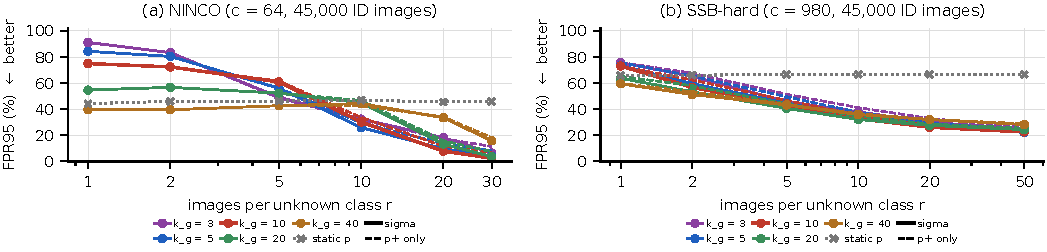
\includegraphics[width=\textwidth]{figs/fig18_kg.pdf}
\caption{近傍数$k_g$を変えた再出現の格子（\FPR{}，交差適合した$\sigma$，単体，DINOv2 L/14 + DINOv3 L/16）．実線は$\sigma$，破線は$\pP$だけ，灰色の点線は静的$p$（$k_g$に依らない）．}
\label{fig:kg}
\end{figure*}

\section{種の上限$\tau$}
\label{sec:app_cap}
命題3が抑えるのは種に混じるIDの\textit{割合}であり，未知が大半を占めるテスト集合では割合$q$の種がIDのほぼ全数になる（\secref{in200}）．そこで，step-upの臨界値を$c_i=\min(q\,i/m,\,\tau)$（Storey型では$q/\hat{\pi}_0$）に置き換えた規則も用意した．棄却された$p$はすべて$\tau$以下なので種に混じるIDの\textit{数}の期待値は$\tau m_0$以下であり，単純BH法では$p\le q\,i^*/m$（$i^*$は棄却数）も満たすので，PRDSのもとで自己整合な手続きとしてFDR$\le q\,m_0/m$が保たれる~\cite{blanchard2008two}．$\tau{=}0.05$は選ばずに固定した．この規則（$\tau{=}0.05$，$q{=}0.2$）は交差適合した$\sigma$について実行前に登録し，上限なしと同じ実行の中で評価した（付録\ref{sec:app_hyp}）．$\sR$との組合せは評価していない．

\textbf{ImageNet-1Kでは変わらない．}上限が効くのはStorey型の閾値が$\tau$を超えるSSB-hardとOpenImage-O（iNaturalistではわずか）で，SSB-hardでは種が折の\NCapSeedSsbHardStoreyRatio\%から\NCapSeedSsbHardStoreycRatio\%に減り，種に混じるIDの割合は\NCapSeedSsbHardStoreyIdfrac{}から\NCapSeedSsbHardStoreycIdfrac{}になる．near-OODの\FPR{}は単体で\NCapStoreycAloneNearFpr\%（上限なし\NAloneNearFpr\%，対応のある差\NCapStoreycAloneNearDfprVsStorey{}），$\times$TINSで\NCapStoreycNearFpr\%（+\NCapStoreycNearDfprVsStorey{}），far-OODとFour-OODの単体は\NCapStoreycAloneFarFpr\%，\NCapStoreycAloneFourFpr\%で，いずれも上限なしと0.25ポイント以内である．

\textbf{混入率が高いベンチマークでは害がほぼ消える．}ImageNet-200のnear-OODでは\FPR{}が\NInTwoZeroZeroMainNearFpr\%から\NInTwoZeroZeroStoreycNearFpr\%へ下がり（差\NInTwoZeroZeroStoreycNearDfprVsStorey{} [\NInTwoZeroZeroStoreycNearDfprVsStoreyLo, \NInTwoZeroZeroStoreycNearDfprVsStoreyHi]），交差適合した$\pP$だけ（\NInTwoZeroZeroLpNearFpr\%）より\NInTwoZeroZeroStoreycNearDfprVsLpAbs{}ポイント低い（[\NInTwoZeroZeroStoreycNearDfprVsLpLo, \NInTwoZeroZeroStoreycNearDfprVsLpHi]）．far-OODは\NInTwoZeroZeroStoreycFarFpr\%で交差適合した$\pP$だけ（\NInTwoZeroZeroLpFarFpr\%）と並ぶ．CIFAR-100ではnear-OODが\NCifarMainNearFpr\%から\NCifarStoreycNearFpr\%（交差適合した$\pP$だけ\NCifarLpNearFpr\%），far-OODが\NCifarMainFarFpr\%から\NCifarStoreycFarFpr\%になり，交差適合した$\pP$だけ（\NCifarLpFarFpr\%）との差は+\NCifarMainFarDfprVsLp{}から+\NCifarStoreycFarDfprVsLp{} [\NCifarStoreycFarDfprVsLpLo, \NCifarStoreycFarDfprVsLpHi]ポイントに縮む．\secref{rec}の格子の\NCaprecNCells{}条件でも，上限付きの規則が$\pP$だけより1ポイント以上悪い条件は混入率30\%以上の\NCaprecNHi{}条件で\NCaprecStoreycHiNWorseLpOne{}，$r\ge10$・混入率30\%未満の\NCaprecLoROneZeroN{}条件では上限なしとの差が最大\NCaprecLoROneZeroMaxStoreycMinusStorey{}ポイントと利得を保つ．

\textbf{位置づけ．}v18--v21では，上限付きの種がImageNet-1Kで上限なしと変わらず，混入率の高いベンチマークで$\pP$だけと同等以上になることから，混入率が未知の運用に上限付きを推していた．$\sR$と上限の組合せは評価していないので，本稿の推奨は結論のとおりとし，上限付きの規則は$\sigma$で登録した変種として報告する．以下の格子の値も$\sigma$のものである．


\tabref{caprec}に，上限付きの規則を\secref{rec}の格子の全条件で評価した\FPR{}を示す（交差適合した$\sigma$，単体，3回の平均）．混入率が低い条件ではStorey型の閾値が$\tau$に達せず，上限付きと上限なしの値は一致する．混入率30\%以上の\NCaprecNHi{}条件（SSB-hard 980クラス$\times$20，50枚）では上限付きのStorey型は$\pP$だけより\NCaprecStoreycHiMaxMinusLpAbs{}--\NCaprecStoreycHiMinMinusLpAbs{}ポイント良く，980クラス$\times$50枚では種に混じるIDの割合が\NCaprecSsbHardCNineEightZeroRFiveZeroStoreyIdfrac{}から\NCaprecSsbHardCNineEightZeroRFiveZeroStoreycIdfrac{}に下がる．全\NCaprecNCells{}条件で上限付きのStorey型が$\pP$だけより1ポイント以上悪いのは\NCaprecStoreycAllNWorseLpOne{}条件（NINCO $c{=}10,20$の$r{=}10$；上限なしも同じ値）で，そこでは種が数十枚しか選ばれず，その\NCaprecNincoCOneZeroROneZeroStoreycIdfracPct\%がIDである（未知がごく少なく$\hat\pi_0$が小さく出る条件；単純BH法は種を選ばない）．単純BH法は上限の有無に依らず全条件で$\pP$だけより最大\NCaprecBhcAllMaxMinusLp{}ポイントしか悪くならない．登録時の仮説H3（付録\ref{sec:app_hyp}：混入率30\%以上で$\pP$だけより1ポイント以上悪くならず，$r\ge10$・混入率30\%未満で上限なしの利得を1ポイント以内に保つ）は，後者の\NCaprecLoROneZeroN{}条件での差が最大\NCaprecLoROneZeroMaxStoreycMinusStorey{}ポイントであり，成り立つ．


\begin{table*}[htbp]
\centering
\caption{種の上限$\tau{=}0.05$の規則の格子（\FPR{}[\%]，交差適合した$\sigma$，単体，3回の平均）．Storey型・単純BH法はそれぞれ上限なし／あり．種はDINOv3 L/16のビューで上限付きStorey型に選ばれた枚数（2つの折の合計）とそのうちIDの割合（\%）．}
\label{tab:caprec}
\vspace{1.5mm}
{\fontsize{6.3pt}{7.4pt}\selectfont\renewcommand{\arraystretch}{1.0}%
\setlength{\tabcolsep}{2.2pt}\begin{tabular}{@{}rrr|cc|cc|c|c|cc@{}}
\hline
\rule[-2.0pt]{0pt}{8.2pt} & & & \multicolumn{2}{c|}{Storey型} & \multicolumn{2}{c|}{単純BH法} & & & \multicolumn{2}{c}{種（上限付きStorey型）} \\
\rule[-2.0pt]{0pt}{8.2pt}$c$ & $r$ & 混入率 & 上限なし & $\tau{=}0.05$ & 上限なし & $\tau{=}0.05$ & $\pP$のみ & 静的$p$ & 枚数 & ID \\
\hline
\multicolumn{10}{@{}l}{\rule{0pt}{6.6pt}\textit{NINCO}} \\
5 & 1 & 0.0 & 73.3 & 73.3 & 73.3 & 73.3 & 73.3 & 33.3 & 0 & -- \\
5 & 2 & 0.0 & 76.7 & 76.7 & 76.7 & 76.7 & 76.7 & 63.3 & 0 & -- \\
5 & 5 & 0.1 & 76.0 & 76.0 & 76.0 & 76.0 & 76.0 & 46.7 & 0 & -- \\
5 & 10 & 0.1 & 40.7 & 40.7 & 40.7 & 40.7 & 40.7 & 69.3 & 35 & 81.9 \\
5 & 20 & 0.2 & 11.7 & 11.7 & 9.7 & 9.7 & 10.7 & 43.3 & 91 & 71.2 \\
5 & 30 & 0.3 & 10.9 & 10.9 & 12.0 & 12.0 & 14.4 & 34.2 & 189 & 58.8 \\
10 & 1 & 0.0 & 73.3 & 73.3 & 73.3 & 73.3 & 73.3 & 33.3 & 0 & -- \\
10 & 2 & 0.0 & 78.3 & 78.3 & 78.3 & 78.3 & 78.3 & 55.0 & 0 & -- \\
10 & 5 & 0.1 & 70.7 & 70.7 & 70.7 & 70.7 & 70.7 & 52.7 & 0 & -- \\
10 & 10 & 0.2 & 28.7 & 28.7 & 26.7 & 26.7 & 26.7 & 45.7 & 70 & 79.1 \\
10 & 20 & 0.4 & 8.8 & 8.8 & 10.0 & 10.0 & 10.7 & 39.2 & 232 & 53.8 \\
10 & 30 & 0.7 & 1.4 & 1.4 & 2.0 & 2.0 & 4.9 & 35.1 & 436 & 50.3 \\
20 & 1 & 0.0 & 60.0 & 60.0 & 60.0 & 60.0 & 60.0 & 35.0 & 0 & -- \\
20 & 2 & 0.1 & 77.5 & 77.5 & 77.5 & 77.5 & 77.5 & 40.0 & 0 & -- \\
20 & 5 & 0.2 & 68.0 & 68.0 & 68.0 & 68.0 & 68.0 & 45.7 & 0 & -- \\
20 & 10 & 0.4 & 36.2 & 36.2 & 34.7 & 34.7 & 34.7 & 44.5 & 35 & 71.7 \\
20 & 20 & 0.9 & 9.0 & 9.0 & 8.5 & 8.5 & 11.8 & 52.5 & 415 & 46.1 \\
20 & 30 & 1.3 & 3.9 & 3.9 & 4.3 & 4.3 & 6.9 & 45.6 & 955 & 48.8 \\
40 & 1 & 0.1 & 75.8 & 75.8 & 75.8 & 75.8 & 75.8 & 47.5 & 0 & -- \\
40 & 2 & 0.2 & 70.8 & 70.8 & 70.8 & 70.8 & 70.8 & 46.2 & 0 & -- \\
40 & 5 & 0.4 & 67.8 & 67.8 & 67.8 & 67.8 & 67.8 & 46.5 & 0 & -- \\
40 & 10 & 0.9 & 35.2 & 35.2 & 34.5 & 34.5 & 34.5 & 48.9 & 175 & 58.5 \\
40 & 20 & 1.7 & 9.8 & 9.8 & 10.2 & 10.2 & 12.9 & 49.8 & 1081 & 47.5 \\
40 & 30 & 2.6 & 2.7 & 2.7 & 3.2 & 3.2 & 5.9 & 45.1 & 1766 & 41.5 \\
64 & 1 & 0.1 & 75.0 & 75.0 & 75.0 & 75.0 & 75.0 & 44.3 & 0 & -- \\
64 & 2 & 0.3 & 72.4 & 72.4 & 72.4 & 72.4 & 72.4 & 46.1 & 0 & -- \\
64 & 5 & 0.7 & 60.9 & 60.9 & 61.6 & 61.6 & 61.6 & 46.2 & 33 & 74.5 \\
64 & 10 & 1.4 & 30.2 & 30.2 & 30.5 & 30.5 & 33.7 & 46.9 & 296 & 46.2 \\
64 & 20 & 2.8 & 7.9 & 7.9 & 7.7 & 7.7 & 11.7 & 45.5 & 1689 & 41.5 \\
64 & 30 & 4.1 & 2.5 & 2.5 & 2.9 & 2.9 & 6.7 & 46.0 & 2664 & 36.6 \\
\multicolumn{10}{@{}l}{\rule{0pt}{6.6pt}\textit{SSB-hard}} \\
10 & 1 & 0.0 & 90.0 & 90.0 & 90.0 & 90.0 & 90.0 & 66.7 & 0 & -- \\
10 & 2 & 0.0 & 86.7 & 86.7 & 86.7 & 86.7 & 86.7 & 73.3 & 0 & -- \\
10 & 5 & 0.1 & 82.0 & 82.0 & 82.0 & 82.0 & 82.0 & 53.3 & 0 & -- \\
10 & 10 & 0.2 & 60.0 & 60.0 & 60.0 & 60.0 & 60.0 & 63.3 & 0 & -- \\
10 & 20 & 0.4 & 45.8 & 45.8 & 47.0 & 47.0 & 46.8 & 69.8 & 122 & 64.8 \\
10 & 50 & 1.1 & 11.5 & 11.5 & 11.1 & 11.1 & 18.1 & 65.7 & 535 & 48.5 \\
30 & 1 & 0.1 & 71.1 & 71.1 & 71.1 & 71.1 & 71.1 & 55.6 & 0 & -- \\
30 & 2 & 0.1 & 82.8 & 82.8 & 82.8 & 82.8 & 82.8 & 65.0 & 0 & -- \\
30 & 5 & 0.3 & 79.1 & 79.1 & 79.1 & 79.1 & 79.1 & 65.1 & 0 & -- \\
30 & 10 & 0.7 & 60.7 & 60.7 & 60.3 & 60.3 & 60.3 & 58.9 & 72 & 77.0 \\
30 & 20 & 1.3 & 43.3 & 43.3 & 43.5 & 43.5 & 46.4 & 71.0 & 344 & 51.4 \\
30 & 50 & 3.2 & 16.5 & 16.5 & 16.3 & 16.3 & 25.1 & 67.3 & 1507 & 41.9 \\
100 & 1 & 0.2 & 80.0 & 80.0 & 80.0 & 80.0 & 80.0 & 65.0 & 0 & -- \\
100 & 2 & 0.4 & 84.0 & 84.0 & 84.0 & 84.0 & 84.0 & 71.0 & 0 & -- \\
100 & 5 & 1.1 & 76.1 & 76.1 & 75.8 & 75.8 & 75.8 & 70.3 & 33 & 87.9 \\
100 & 10 & 2.2 & 50.7 & 50.7 & 51.5 & 51.5 & 56.5 & 68.1 & 404 & 55.2 \\
100 & 20 & 4.3 & 32.4 & 32.4 & 33.3 & 33.3 & 38.5 & 66.9 & 1597 & 44.2 \\
100 & 50 & 10 & 18.5 & 18.5 & 18.7 & 18.7 & 24.2 & 67.2 & 5132 & 31.6 \\
300 & 1 & 0.7 & 78.6 & 78.6 & 78.6 & 78.6 & 78.6 & 67.1 & 0 & -- \\
300 & 2 & 1.3 & 73.6 & 73.6 & 73.6 & 73.6 & 73.6 & 64.7 & 0 & -- \\
300 & 5 & 3.2 & 58.9 & 58.9 & 58.7 & 58.7 & 62.2 & 64.6 & 402 & 49.7 \\
300 & 10 & 6.2 & 42.3 & 42.3 & 42.8 & 42.8 & 47.9 & 66.8 & 1751 & 38.0 \\
300 & 20 & 12 & 29.7 & 29.7 & 29.9 & 29.9 & 34.2 & 65.7 & 5348 & 32.2 \\
300 & 50 & 25 & 19.3 & 19.6 & 19.6 & 19.6 & 22.1 & 66.9 & 14736 & 19.1 \\
980 & 1 & 2.1 & 73.1 & 73.1 & 72.9 & 72.9 & 72.9 & 65.9 & 33 & 84.7 \\
980 & 2 & 4.2 & 56.8 & 56.8 & 56.5 & 56.5 & 62.4 & 66.1 & 522 & 47.5 \\
980 & 5 & 9.8 & 43.1 & 43.1 & 42.7 & 42.7 & 46.7 & 66.6 & 3381 & 36.1 \\
980 & 10 & 18 & 32.8 & 32.8 & 32.6 & 32.6 & 35.5 & 66.7 & 9372 & 31.0 \\
980 & 20 & 30 & 26.2 & 26.1 & 26.1 & 26.1 & 27.8 & 66.8 & 17485 & 16.7 \\
980 & 50 & 52 & 22.6 & 22.2 & 21.5 & 22.2 & 23.4 & 66.6 & 40958 & 6.6 \\
\hline
\end{tabular}}%

\end{table*}

\section{追加実験の事前登録と仮説の判定}
\label{sec:app_hyp}
付録\ref{sec:app_cap}の上限付きの種，\secref{in200}の全学習画像・ゼロショットの基線，付録\ref{sec:app_kg}の$k_g$の格子，付録\ref{sec:app_views}の中心化は，1つの登録文書（公開リポジトリの\texttt{experiments/phase15/prereg\_p15.json}，SHA-256 \texttt{83ea4061}$\cdots$）に計算の内容・報告の形・6つの仮説を記してから実行した．登録文書は評価の実行前に公開リポジトリのブランチ\texttt{phase12-15-registrations}（コミット\texttt{8ef9c8d}）に置いた（学習画像の特徴抽出だけはその前に始めた）．構成の選択は行わず（$\tau$と$q$は固定，主構成は変えない），登録からの逸脱はない．系1の実測（付録\ref{sec:app_kg}）は査読後に加えた登録外の記述的な計算で，選択を含まない．判定は次のとおりである（いずれも交差適合した$\sigma$についての仮説）．
\begin{itemize}
\item \textbf{H1}（上限は害を消す：CIFAR-100 far-OODとImageNet-200 near-OODで上限付きの規則は$\pP$だけの+0.5ポイント以内）：成立（+\NCifarStoreycFarDfprVsLp{}，\NInTwoZeroZeroStoreycNearDfprVsLp{}ポイント）．
\item \textbf{H2}（上限はImageNet-1K near-OODで上限なしの0.5ポイント以内）：成立（単体\NCapStoreycAloneNearDfprVsStorey{}，$\times$TINS +\NCapStoreycNearDfprVsStorey{}ポイント）．
\item \textbf{H3}（格子：混入率30\%以上で$\pP$だけより1ポイント以上悪くならず，$r\ge10$・混入率30\%未満で上限なしの利得を1ポイント以内に保つ）：成立（付録\ref{sec:app_cap}）．
\item \textbf{H4}（全学習画像のkNN（$k{=}50$）は両ベンチマークで16枚の静的$p$より良く，ImageNet-200のnear-OODでは$\sigma$がkNNより低い\FPR{}を保つ）：前半は否定（ImageNet-200でkNN \NInTwoZeroZeroKnnAllKFiveZeroNearFpr\%／\NInTwoZeroZeroKnnAllKFiveZeroFarFpr\%対静的$p$ \NInTwoZeroZeroStaticNearFpr\%／\NInTwoZeroZeroStaticFarFpr\%，CIFAR-100のfar-OODで\NCifarKnnAllKFiveZeroFarFpr\%対\NCifarStaticFarFpr\%；CIFAR-100のnear-OODだけ\NCifarKnnAllKFiveZeroNearFpr\%対\NCifarStaticNearFpr\%），後半は成立（\NInTwoZeroZeroMainNearFpr\%対\NInTwoZeroZeroKnnAllKFiveZeroNearFpr\%）．
\item \textbf{H5}（$\sigma$が静的$p$を下回る$r$は$k_g$が小さいほど小さく，大きい$r$での利得は$k_g\in\{10,20\}$で最大）：前半は否定，後半は$\{5,10\}$として部分的に成立（付録\ref{sec:app_kg}）．
\item \textbf{H6}（中心化でCLIPの静的$p$はDINO系の範囲（near 70\%未満，far 40\%未満）に入り，DINO系の変化は10ポイント以内）：前半は否定（near \NViewClipStaticcNearFpr\%，far \NViewClipStaticcFarFpr\%），後半は静的$p$で成立（最大\NViewsDinoCentredMaxabsFpr{}ポイント），kNNではDINO (v1)のfar-OODで\NViewsDinoKnncentredMaxabsFpr{}ポイント動く．
\end{itemize}

\textbf{一つの量の変種（付録\ref{sec:app_h16}）．}開発用分割dev1だけで\NHsExplNCfg{}通りの構成を探索した後，構成，ベース検出器との積の形を選ぶ規則，dev2での3つの仮説，採否の規則を登録文書（\texttt{experiments/phase16/prereg\_p16.json}，SHA-256 \texttt{2e16ae0c}$\cdots$）に記し，公開リポジトリのブランチ\texttt{phase12-15-registrations}（コミット\texttt{6bbae3d}）で公開されたことを確かめてから実行した（2026年10月11日12:56 UTC）．H1--H3はdev2ですべて成立し，登録した規則では$h$が主構成になる．しかしテスト集合では$\sigma$に劣ったため（\tabref{h16}），$\sigma$を主構成のまま$h$を変種として報告した（v19--v21）．これは登録からの逸脱であり，判断はテスト集合の値を見た後に行った（「結果が良ければ本文，悪ければ付録」とすることは実行前に決めていたが，登録文書には書いていない）．採否の規則は点推定（dev2の差が+0.5以下）で定めていた．dev2の差の区間の上端は+\NRHsUpperNear{}，+\NRHsUpperFar{}で，上端で判定していれば$h$は採用されず，この逸脱は生じなかった．修正記録は\texttt{experiments/phase16/prereg\_p16\_amendments.json}にある．

\textbf{参照画像による読み出し（付録\ref{sec:app_p17}）．}$\sR$，その採否の規則（区間の上端による），記述的な解析を登録文書（\texttt{experiments/phase17/prereg\_p17.json}）に記し，公開を確かめてから実行した．規則はdev2で成り立ち，$\sR$を主構成にした．登録からの逸脱はない．

% v22: the one-quantity read-out h16 as a registered variant in the appendix (the main read-out is sigma_ref).
\section{一つの量としての読み出し（登録した変種）}
\label{sec:app_h16}
v18--v21の読み出し$\sigma$（付録\ref{sec:app_p17}）は，支持画像と種からの2本の伝播の較正順位を掛け，2つの折で交差適合したものである．これを一つの量「画像から出たランダムウォークは支持画像と種のどちらに先に着くか」に置き換える読み出し$h$を，開発用分割dev1での探索の後に登録し，dev2で確認し，テスト集合で構成を凍結したまま評価した（付録\ref{sec:app_hyp}）．dev2では登録した仮説がすべて成立したが，ベンチマークでは$\sigma$に及ばなかった（\tabref{h16}）．参照画像で種を選び折を使わない仕組みは$h$から取り出して$\sR$に使った（\secref{ref}）．

\subsection{定義}
\label{sec:h19def}
支持画像$\mathcal{S}$，参照画像$\mathcal{R}$，較正画像$\mathcal{C}$，テスト画像$\mathcal{T}$のすべてを節点とする．ビュー$v$ごとに，各節点からコサイン類似度の上位$k_g{=}10$の節点へ重み$a^v_{ij}=\max(f_v(x_i)^{\top}f_v(x_j),0)$の辺を張って$W_v=\max(A_v,A_v^{\top})$とし，それぞれの次数の中央値で割って足した$W=\sum_vW_v/\mathrm{med}_i\,\delta^v_i$を1つのグラフとする（次数$\delta_i=\sum_jW_{ij}$，$P=D^{-1}W$）．$\mathcal{R}$，$\mathcal{C}$，$\mathcal{T}$はすべてラベルのない節点として同じ扱いを受け，グラフは節点の名札に依らない．

このグラフの上で，節点$i$に平均$1/\delta_i$の指数時間とどまり，確率$P_{ij}$で$j$へ跳ぶ連続時間のランダムウォーク$X_t$を考える．ランダムウォークはジャンプのたびに確率$1-\lambda$で，また単位時間あたり率$\gamma$で消える．支持画像と種$\hat{Q}$（\secref{seed19}）を吸収壁とし，
\begin{equation}
\begin{aligned}
h(x)&=\Pr\nolimits_x\big(\text{消える前に，}\hat{Q}\text{より先に}\mathcal{S}\text{に着く}\big)\\
&=\mathbb{E}_x\big[\lambda^{N}e^{-\gamma T};\,\tau_{\mathcal{S}}<\tau_{\hat{Q}}\big]
\end{aligned}
\label{eq:h}
\end{equation}
を画像$x$のIDらしさとする（$\tau_A$は集合$A$に初めて着く時刻，$N$と$T$はそこまでのジャンプの回数と時間）．$h$は「支持画像に着く」「種に着く」「消える」という排反な3つの行き先のうち，支持画像が最初になる確率であり，3つの確率の和は1である（付録\ref{sec:app_h19}）．$\lambda{=}1,\gamma{=}0$では調和関数~\cite{zhu2003harmonic}やランダムウォーカーによる領域分割~\cite{grady2006rw}の到達確率，一般には部分吸収ランダムウォーク~\cite{wu2012parw}の一つの形である．

\textbf{\TFaces（三つの表示）．}自由な節点を$F=V\setminus(\mathcal{S}\cup\hat{Q})$とすると，次の3つは同じ$h$を与える．(i) 確率\eqnref{h}．(ii) 連立一次方程式$(D+\gamma I-\lambda W)_{FF}\,h_F=\lambda W_{F\mathcal{S}}\mathbf{1}$（係数行列は対称正定値）．(iii) $f|_{\mathcal{S}}=1$，$f|_{\hat{Q}}=0$のもとで
\begin{equation}
\mathcal{E}(f)=\lambda\sum_{i<j}W_{ij}(f_i-f_j)^2+\sum_i\big((1-\lambda)\delta_i+\gamma\big)f_i^2
\label{eq:energy}
\end{equation}
を最小にする$f$．これは辺に伝導度$\lambda W_{ij}$，各節点と接地の間に伝導度$(1-\lambda)\delta_i+\gamma$の漏れを置いた抵抗回路で，支持画像を電位1，種を接地したときの電位である~\cite{doyle1984}（証明は付録\ref{sec:app_h19}）．

\textbf{二つの代価．}\eqnref{energy}の漏れ$(1-\lambda)\delta_i$は次数に比例するので，これだけなら$W$を定数倍しても$h$は変わらず，$h$はグラフの形（$P$）だけで決まる．漏れ$\gamma$は絶対的で，次数の小さい疎な節点ほど流れの多くを失う．1回の訪問で消えずに次へ跳ぶ確率$\rho_x=\lambda\delta_x/(\delta_x+\gamma)$は疎な節点で小さい．$h(cW;\lambda,c\gamma)=h(W;\lambda,\gamma)$なので，$\gamma$は次数の中央値に対する比$g$で置き，$h$を重みの全体の尺度に依らない量にする．

\textbf{\TLimits（二つの代価の極限）．}(i) 種がなく，$\lambda=1-\mu\varepsilon$，$\gamma=\nu\varepsilon$（$\mu,\nu\ge0$）とすると，$\varepsilon\to0$で$(1-h(x))/\varepsilon\to\mu\,\mathbb{E}_x[N_{\mathcal{S}}]+\nu\,\mathbb{E}_x[T_{\mathcal{S}}]$である（$N_{\mathcal{S}}$，$T_{\mathcal{S}}$は支持画像に着くまでの歩数と時間）．(ii) 支持画像に置いた質量を伝播させる局所・大域一貫性~\cite{zhou2004lgc}の解$u=(1-\lambda)(I-\lambda D^{-1/2}WD^{-1/2})^{-1}\mathbf{1}_{\mathcal{S}}$は，連結なグラフで$\lambda\to1$のとき$\sqrt{\boldsymbol{\delta}}$に比例する量に収束する．

\textbf{形と密度．}(i)から，代価の小さい極限で種のない$h$の順位は，支持画像に着くまでの期待費用「1歩あたり$\mu$，時間あたり$\nu$」で決まる．ランダムウォークは節点$i$に平均$1/\delta_i$とどまるので，時間は経路の疎さを，歩数はたどる近傍の段数を測る．支持画像と疎にしかつながらない未知の塊（near-OOD）は形の現象，IDから離れた疎な領域（far-OOD）は密度の現象であり，二つの代価が一本のランダムウォークの上でそれぞれを測る（\figref{toy}）．支持画像を吸収壁にしない伝播(ii)は，ランダムウォークが支持画像を通り抜けて定常分布に近づくため次数だけの量に退化するが，$h$は支持画像に着いた時点で止まる．

% 付録は1段組：模式図は浮動させず，定義の節の終わりに置く（読み出しの手順の途中に入らないように）
\par\medskip
\noindent\begin{minipage}{\linewidth}
\centering
\makeatletter\def\@captype{figure}\capwidth\hsize\ecapwidth\hsize\abovecaptionskip1mm\belowcaptionskip\z@\makeatother
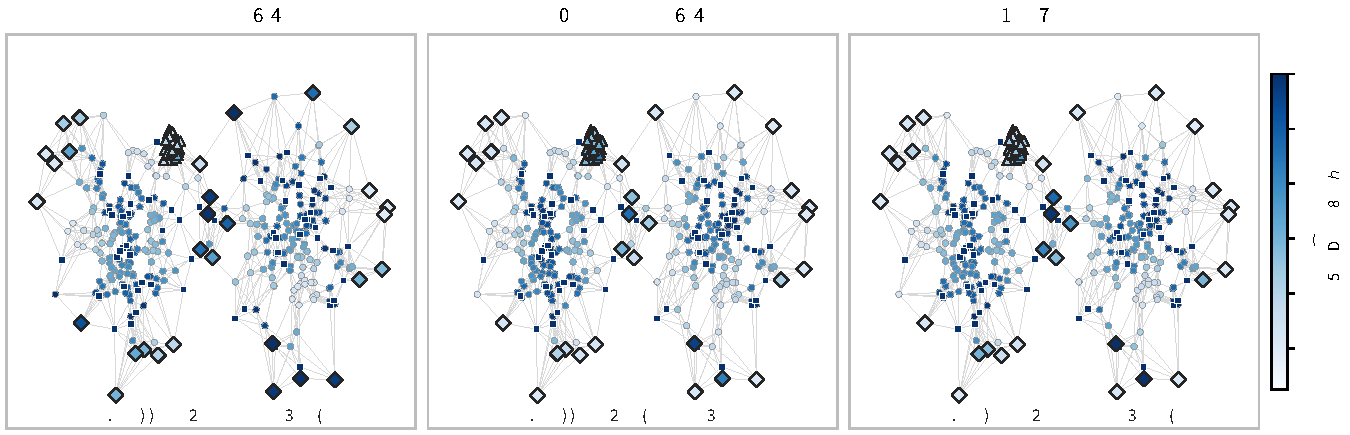
\includegraphics[width=0.86\linewidth]{figs/fig_toy19.pdf}
\caption{同じ量$h$と二つの代価（2次元の模式例；ガウス重みの対称な$k$近傍グラフ，$k{=}8$）．■は支持画像，○はIDのラベルなし画像，▲は密な未知の塊，◆は疎に散らばった未知で，色はラベルなし画像の中での$h$の順位（薄いほどOODらしい）．(a) 歩数の代価だけ（$\lambda{=}0.8$，$\gamma{=}0$）は塊を捉えるが散らばった未知を逃し，(b) 時間の代価だけ（$\lambda{=}1$，$\gamma$は次数の中央値の0.3倍）はその逆になり，(c) 二つの代価（$\lambda{=}0.8$，$\gamma$は0.03倍）は両方をIDより下に置く．種は使っていない．}
\label{fig:toy}
\end{minipage}
\par\medskip


\subsection{種と較正順位}
\label{sec:seed19}
ラベル付き画像をクラスごとに支持画像12枚，参照画像2枚，較正画像2枚に，画像に依らない位置で分ける．(1) 種のない$h$を$h^{(0)}$とし，プール$\mathcal{U}=\mathcal{C}\cup\mathcal{T}$の各画像を参照画像の中での順位$p_{\mathcal{R}}(u)=(1+|\{r\in\mathcal{R}:h^{(0)}(r)\le h^{(0)}(u)\}|)/(|\mathcal{R}|+1)$で読む．(2) $p_{\mathcal{R}}$にStorey型のBH法~\cite{benjamini1995bh,storey2002}（水準$q{=}0.2$）をかけ，棄却された画像を種$\hat{Q}\subset\mathcal{U}$とする（較正画像も候補に入る）．(3) 種を吸収壁にした$h$を解き，すべてのラベルなし画像を一歩先読みの値
\begin{equation}
s(x)=\rho_x\,(Ph)(x)=\frac{\lambda(Wh)(x)}{\delta_x+\gamma}
\label{eq:s}
\end{equation}
で採点する．種でない画像では$s=h$，種では「一歩跳んだ後に種より先に支持画像に着く確率」（自分に戻れば種に着いたとみなす）である．(4) $s$の較正画像の中での順位
\begin{equation}
p(x)=\frac{1+|\{x'\in\mathcal{C}:s(x')\le s(x)\}|}{|\mathcal{C}|+1}
\label{eq:p}
\end{equation}
を判定に，$s$を順位付けに使う．較正画像の集合は1つなので$p$は$s$の単調関数であり，二つは同点を除いて同じ順序を与える．計算は疎な正定値系2本を共役勾配法で解くだけである．

\textbf{\TValid（有効性）．}較正画像とIDのテスト画像が，他のすべての画像を所与として交換可能なら，(i) IDのテスト画像$x$について$\Pr(p(x)\le\alpha)\le\alpha$，(ii) $\{p(x)\}_{x\in\mathcal{T}}$はIDの画像の上でPRDSであり，水準$q$のBH法で選んだ集合の偽発見率は$q\,m_0/m$以下，Storey型では$q$以下である（$m_0$はIDのテスト画像の数）．(iii) さらに参照画像とプールのIDの画像が交換可能なら，種の偽発見率も$q$以下である．$s$は$\mathcal{S}$，$\mathcal{R}$と$\mathcal{U}$の画像の特徴の集まり（順序なし）だけの関数で，$\mathcal{U}$の中でどの画像を較正画像と呼ぶかに依らない．これはAdaDetect~\cite{marandon2024adadetect}の条件であり，$p$は同論文の経験$p$値である（付録\ref{sec:app_h19}）．種を$\mathcal{T}$だけから$\mathcal{C}$に対する順位で選ぶと$s$が較正画像の名札に依存して条件が崩れる．参照画像を分けて較正画像も種の候補にすることで，較正画像とテスト画像を折に分けずに保証が得られる．


\subsection{逃げる確率と捕まる確率}
\label{sec:sep19}
両側の評価は一つの関数
\begin{equation}
\varphi(\rho,a,b)=\frac{\rho\,a}{1-\rho\,(1-a-b)}\qquad(a=0\text{では}\varphi=0)
\label{eq:phi}
\end{equation}
で書ける．$\varphi$は$\rho$と$a$について増加，$b$について減少し，漏れがなければ
\begin{equation*}
\varphi(1,a,b)=\frac{a}{a+b}
\end{equation*}
である．出口$a$と出口$b$の競争に，訪問ごとの生存率$\rho$が掛かる量と読める．

\appblock
\textbf{\TEscape（逃げる確率：未知の側）．}支持画像も種も含まない節点の集合$Q$について，$Q$を初めて出る先が$z$である割引確率を$H_Q(y,z)$とすると，
\begin{equation*}
h(y)=\sum_{z\in\partial Q}H_Q(y,z)\,h(z)\qquad\text{（等式）}
\end{equation*}
であり，種でない外へ逃げる確率
\begin{equation*}
\pi_Q(y)=\sum_{z\in\partial Q\setminus\hat{Q}}H_Q(y,z)
\end{equation*}
について$h(y)\le\pi_Q(y)$である．$y\in Q$の重みのうち種でない外へ向かう割合を$e_y$，種へ向かう割合を$\zeta_y$とすると，
\begin{equation*}
\pi_Q\le\varphi\big(\max_Q\rho,\ \max_Qe,\ \min_Q\zeta\big).
\end{equation*}

\appblock
\textbf{\TCapture（捕まる確率：IDの側）．}支持画像も種も含まない節点の集合$B$について，$y\in B$の重みのうち支持画像へ向かう割合を$\omega_y$，$B$にも支持画像にも属さない節点へ向かう割合を$\eta_y$とすると，$B$を出ずに支持画像に着く確率$\kappa_B$について
\begin{equation*}
h\ge\kappa_B\ge\varphi\big(\min_B\rho,\ \min_B\omega,\ \max_B\eta\big)
\end{equation*}
である．また，すべてのラベルなし画像で
\begin{equation*}
s(x)\ge\rho_x\,\omega_x
\end{equation*}
である．

\appblock
\textbf{\CSep（分離）．}種でないテスト画像$y$が\TEscape{}の$Q$に属し，各較正画像$x'$について$\ell(x')\le s(x')$（例えば$\ell(x')=\rho_{x'}\omega_{x'}$）なら，
\begin{equation}
p(y)\le\frac{1+|\{x'\in\mathcal{C}:\ell(x')\le\pi_Q(y)\}|}{|\mathcal{C}|+1}.
\label{eq:sep}
\end{equation}
特に$\pi_Q(y)<\min_{x'\in\mathcal{C}}\ell(x')$なら$p(y)$は床$1/(|\mathcal{C}|+1)$に落ち，$y$は$\alpha\ge1/(|\mathcal{C}|+1)$のすべての水準でOODと判定される（証明は付録\ref{sec:app_h19}）．

\appblock
\textbf{読み方．}未知の塊では「種でない外への辺」と「種への辺」が競い，IDの近傍では「支持画像への辺」と「漏れる辺」が競う．同じ$\varphi$が両側を抑え，その大小が較正順位の分離\eqnref{sep}を決める．有効性（\TValid）と検知力（\TEscape{}--\CSep）は同じ量$s$についての主張である．種を増やすと$h$は単調に減り，塊のどの節点でも重みの割合$\zeta$以上が種へ向かえば，漏れがなくても逃げる確率は
\begin{equation*}
\pi_Q\le\frac{\max_Qe}{\max_Qe+\zeta}
\end{equation*}
を満たす．同じ未知クラスの画像が複数枚あるとき，種になった画像は残りの画像の重みの一部を占め，その逃げる確率を下げる．これが自己ラベル付けの効く理由である．


\subsection{結果}
\label{sec:app_h16res}
\textbf{登録と判定．}開発用分割dev1で\NHsExplNCfg{}通りの構成を探索した後，構成を1つに固定し（$\lambda{=}0.95$，$g{=}1/16$，ビューの重みを次数の中央値で割った和のグラフ，クラスあたり支持12・参照2・較正2，$q{=}0.2$，折なし），ベース検出器との積の形を選ぶdev1の規則，dev2での3つの仮説，採否の規則を登録してから実行した（付録\ref{sec:app_hyp}）．dev1の規則は積を$s_0\cdot p$に決めた（$s_0\cdot s$は$\times$TINSのfar-OODが\NHsDevOneTinsFarS\%で$\sigma$の\NHsDevOneTinsSigFar\%+0.5を超える）．dev2ではH1（near-OODの\FPR{}の差が+0.5以下）が\NHsDevTwoNearD{}，H2（far-OOD）が\NHsDevTwoFarD{}，H3（$p$の誤警報率が$\alpha{=}0.05$で0.06以下，$0.2$で0.21以下）が\NHsDevTwoFprFive{}／\NHsDevTwoFprTwenty{}とすべて成立し，登録した規則では$h$を主構成にすることになった．ただし\AUC{}は$\sigma$より低く（\NHsDevTwoNearDAuc{} [\NHsDevTwoNearDAucLo, \NHsDevTwoNearDAucHi]，\NHsDevTwoFarDAuc{} [\NHsDevTwoFarDAucLo, \NHsDevTwoFarDAucHi]ポイント），\FPR{}の差の区間の上端はnear +\NRHsUpperNear{}，far +\NRHsUpperFar{}と+0.5を超えていた．規則は点推定で判定したので$h$が採用されたが，区間の上端で判定していれば採用されなかった．

\begin{table*}[htbp]
\centering
\caption{一つの量$h$（登録した構成）と交差適合した$\sigma$（単体，ベンチマークは6通りの抽出の平均，dev2は5通り；差は$h-\sigma$，抽出を単位とする対応のある95\% $t$区間）．$\times$TINSの$h$はdev1の規則で選んだ$s_0\cdot p$．}
\label{tab:h16}
\vspace{1.5mm}
{\fontsize{6.5pt}{7.6pt}\selectfont\renewcommand{\arraystretch}{1.0}%
\setlength{\tabcolsep}{1.7pt}\begin{tabular}{@{}lcc|cc|c@{}}
\hline
\rule[-2.0pt]{0pt}{8.6pt} & \multicolumn{2}{c|}{$\sigma$（交差適合）} & \multicolumn{2}{c|}{一つの量$h$} & \\
\rule[-2.0pt]{0pt}{8.6pt}設定 & \AUC & \FPR & \AUC & \FPR & \FPR{}の差 [95\%区間] \\
\hline
dev2 near（登録した確認） & 97.16 & 12.92 & 96.89 & 12.87 & -0.06 [-1.00, +0.89] \\
dev2 far（登録した確認） & 96.56 & 16.73 & 96.18 & 16.98 & +0.25 [-1.04, +1.54] \\
\hline
ImageNet-1K near-OOD & 97.94 & 11.50 & 97.18 & 13.65 & +2.14 [+1.70, +2.58] \\
ImageNet-1K far-OOD & 98.79 & 5.17 & 98.20 & 7.32 & +2.15 [+1.87, +2.42] \\
Four-OOD & 98.80 & 4.56 & 98.04 & 7.00 & +2.44 [+2.06, +2.81] \\
\hline
ImageNet-200 near-OOD & 98.17 & 9.07 & 96.57 & 8.10 & -0.97 [-1.38, -0.56] \\
ImageNet-200 far-OOD & 99.35 & 2.15 & 98.59 & 4.15 & +2.00 [+1.77, +2.23] \\
CIFAR-100 near-OOD & 99.18 & 2.90 & 98.44 & 6.42 & +3.52 [+3.17, +3.87] \\
CIFAR-100 far-OOD & 99.37 & 2.34 & 97.56 & 3.31 & +0.97 [+0.50, +1.44] \\
\hline
ImageNet-1K near-OOD $\times$TINS & 98.09 & 10.50 & 96.75 & 18.58 & +8.09 [+7.54, +8.64] \\
ImageNet-1K far-OOD $\times$TINS & 99.05 & 4.16 & 98.88 & 4.92 & +0.77 [+0.60, +0.93] \\
Four-OOD $\times$TINS & 99.09 & 3.39 & 98.97 & 3.56 & +0.18 [+0.07, +0.28] \\
\hline
\end{tabular}}%

\end{table*}

\textbf{ベンチマーク．}テスト集合では$h$は$\sigma$に及ばない（\tabref{h16}）．ImageNet-1Kの\FPR{}はnear-OODで\NHsTestNearSigFpr\%から\NHsTestNearFpr\%（差\NHsTestNearD{} [\NHsTestNearLo, \NHsTestNearHi]），far-OODで\NHsTestFarSigFpr\%から\NHsTestFarFpr\%，Four-OODで\NHsTestFourSigFpr\%から\NHsTestFourFpr\%になり，\AUC{}はそれぞれ\NRAbsHsTestNearDAucVal{}，\NRAbsHsTestFarDAucVal{}，\NRAbsHsTestFourDAucVal{}ポイント下がる．ImageNet-200のnear-OODだけは\FPR{}が\NRAbsHsInTwoHundredNearDVal{}ポイント良いが\AUC{}は\NRAbsHsInTwoHundredNearDAucVal{}ポイント低く，far-OODとCIFAR-100では悪い．$\times$TINS（$s_0\cdot p$）のnear-OODは\NHsTestNearTinsSigFpr\%から\NHsTestNearTinsFpr\%へ大きく悪化する．$p$の床の上ではベース検出器が未知の順序を決めるためで，本文がベース検出器を$\exp\sR$と掛ける理由（\secref{score}）と同じである．学習画像で較正した$p$の$\alpha{=}0.05$での誤警報率はImageNet-1Kで\NHsTestNearValFive{}／\NHsTestFarValFive{}／\NHsTestFourValFive{}であり，同じ較正の$\pfin$（\NHsTestNearSigValFive{}／\NHsTestFarSigValFive{}／\NHsTestFourSigValFive）より高い（較正画像とテスト画像は交換可能でない；\secref{fdp}）．再出現の格子では\NHsRecNCells{}条件のうち\NHsRecNBetter{}条件で$\sigma$より良いが，同じ未知クラスが1--2枚の\NHsRecNSingleton{}条件では平均\NHsRecSingletonMeanD{}ポイント悪い（NINCOの$c{=}64$，$r{=}1$で\NHsRecNincoCSixtyFourROne\%，$\sigma$は\NHsRecNincoCSixtyFourROneSig\%）．

\textbf{開発用分割から移らなかったこと．}dev2はdev1と同じ作り方で，far-OODの画像集合（OpenImage-O）も共通であり，dev2での非劣性はベンチマークに移らなかった．dev1の探索（探索時のコードの値；$\sigma$の折の割り当ては登録した実行と異なる，付録\ref{sec:app_p17}）では，支持画像と種を吸収壁にして1歩ごとの代価だけを持たせた量はnear-OODで$\sigma$に並ぶがfar-OODで大きく劣り（\FPR{} \NHsExplAbsOneNear\%／\NHsExplAbsOneFar\%，$\sigma$は\NHsExplSigNear\%／\NHsExplSigFar\%；登録した実行の$\sigma$は\NRFcDevOneNearPSixteen\%／\NRFcDevOneFarPSixteen\%），その原因は局所・大域一貫性の質量の次数成分にあった．次数だけをスコアにしても\AUC{}はfar-OODで\NHsExplDegAucFarVTwo\%（DINOv2），\NHsExplDegAucFarVThree\%（DINOv3）に達し，near-OODでは\NHsExplDegAucNearVTwo\%，\NHsExplDegAucNearVThree\%にとどまった（テスト集合では次数だけの\AUC{}はfar-OODでも\NRDecDegINFarAuroc\%で，この手がかりは移らなかった；\tabref{dec}）．時間の代価$\gamma$はこの密度の手がかりを確率の中に戻すために入れたもので，dev1では$\sigma$に並んだ（\NHsExplFinNear\%／\NHsExplFinFar\%）．ベンチマークでは再出現のない未知とfar-OODで劣ることから，$\gamma$による密度の取り込みは本文の伝播の次数成分の代わりとして十分でないと考えられる．

\textbf{系A1の実測．}再出現の格子で，$h\le\pi_Q$（\TEscape）と$\pi_Q\le\bar\phi$はすべての未知画像で成り立つ（付録\ref{sec:app_bounds}の\tabref{bounds}）．$h/\pi_Q$の中央値は\NRBdHOneHOverPiMin--\NRBdHOneHOverPiMax{}で\TEscape{}は緩くないが，\CSep{}を較正画像側の下界$\ell=\rho\omega$で読むと，$\ell$が実際のスコア$s$の\NRBdHOneEllOverSMedMin--\NRBdHOneEllOverSMedMax{}倍しかないため保証される未知は全条件で0である．実際のスコアで読めば最大\NRBdHOneCertSMax\%を保証する．下界側の弱さが，系A1が実際の検知を説明できない主な理由である．

\textbf{位置づけ．}以上から，$\sigma$を主構成のまま$h$を登録した変種として報告した（v19--v21）．これは登録からの逸脱であり，その判断はテスト集合の値を見た後に行った．ただし「結果が良ければ本文，悪ければ付録に置く」ことは実行の前に決めていた（登録文書には書いていない；付録\ref{sec:app_hyp}）．区間の上端で判定する規則なら$h$は採用されず，逸脱は生じなかった．$h$は誤警報率の保証（\TValid）と検知力（\TEscape{}--\CSep）を同じ量について述べられるが，ベンチマークでの性能は$\sigma$にも$\sR$にも及ばない．


\section{一つの量$h$の証明と性質}
\label{sec:app_h19}
記号は\secref{h19def}のとおりで，
\begin{equation*}
M=(D+\gamma I-\lambda W)_{FF},\qquad\rho_x=\frac{\lambda\,\delta_x}{\delta_x+\gamma}
\end{equation*}
とする．

\textbf{\TFaces{}の証明．}

\textit{(i)から(ii)．}$x\in F$で最初の滞在時間$T_1\sim\mathrm{Exp}(\delta_x)$を生き延びる確率は
\begin{equation*}
\mathbb{E}\,e^{-\gamma T_1}=\int_0^{\infty}\delta_x e^{-\delta_x t}\,e^{-\gamma t}\,dt=\frac{\delta_x}{\delta_x+\gamma}
\end{equation*}
であり，続くジャンプを生き延びて$j$へ移る確率は$\lambda P_{xj}$である．よって
\begin{equation*}
h(x)=\frac{\delta_x}{\delta_x+\gamma}\sum_j\lambda P_{xj}\,h(j)=\rho_x\,(Ph)(x)=\frac{\lambda\,(Wh)(x)}{\delta_x+\gamma}\qquad(x\in F)
\end{equation*}
であり，境界の値（$\mathcal{S}$で1，$\hat{Q}$で0）を代入すれば
\begin{equation*}
(\delta_x+\gamma)\,h(x)-\lambda\sum_{j\in F}W_{xj}\,h(j)=\lambda\sum_{j\in\mathcal{S}}W_{xj}\qquad(x\in F),
\end{equation*}
すなわち(ii)の$Mh_F=\lambda W_{F\mathcal{S}}\mathbf{1}$になる．

\textit{一意性．}$M$の非対角成分の行和は
\begin{equation*}
\lambda\sum_{j\in F}W_{xj}\le\lambda\,\delta_x
\end{equation*}
なので，$\gamma>0$，または$\lambda<1$かつ$\delta_x>0$なら$M$は狭義対角優位であり，対称なので正定値である（$\lambda{=}1,\gamma{=}0$では，$F$と交わる各連結成分が境界を含めば既約対角優位）．よって解は一意で，確率\eqnref{h}（方程式の最小の非負解）と一致する．

\textit{(iii)．}$\mathcal{E}$を$f_x$（$x\in F$）で微分すると
\begin{equation*}
\frac{\partial\mathcal{E}}{\partial f_x}=2\Big[(\delta_x+\gamma)f_x-\lambda\sum_jW_{xj}f_j\Big]
\end{equation*}
で，停留条件は(ii)と同じ式であり，ヘッセ行列$2M$は正定値なのでその解が最小点である．回路ではこれが自由な節点でのキルヒホッフの電流則
\begin{equation*}
\sum_j\lambda W_{xj}\,(f_x-f_j)+\big((1-\lambda)\delta_x+\gamma\big)f_x=0
\end{equation*}
にあたる．$\square$

\appblock
\textbf{三つの行き先．}$\mathcal{S}$と$\hat{Q}$の役割を入れ替えた量を$\check h$，どちらにも着く前に消える確率を$d$とすると，$M$が正則なとき
\begin{equation*}
h+\check h+d=1
\end{equation*}
である（$\lambda{=}1,\gamma{=}0$では$\check h=1-h$）．

\textit{証明．}最初の滞在と最初のジャンプで場合を分けると
\begin{equation*}
d(x)=\frac{\gamma}{\delta_x+\gamma}+\frac{\delta_x}{\delta_x+\gamma}\Big[(1-\lambda)+\lambda\sum_{j\in F}P_{xj}\,d(j)\Big]\qquad(x\in F),
\end{equation*}
すなわち$Md_F=\gamma\mathbf{1}+(1-\lambda)\boldsymbol{\delta}_F$である．一方
\begin{align*}
M\mathbf{1}_F&=(1-\lambda)\boldsymbol{\delta}_F+\gamma\mathbf{1}+\lambda W_{F\mathcal{S}}\mathbf{1}+\lambda W_{F\hat{Q}}\mathbf{1},\\
Mh_F&=\lambda W_{F\mathcal{S}}\mathbf{1},\qquad M\check h_F=\lambda W_{F\hat{Q}}\mathbf{1}
\end{align*}
だから
\begin{equation*}
M\big(h+\check h+d\big)_F=M\mathbf{1}_F
\end{equation*}
であり，$M$が正則なので$h+\check h+d=1$である．$\square$

\appblock
\textbf{\TLimits{}の証明．}

\textit{(i)．}種がないので$h(x)=\mathbb{E}_x[\lambda^{N}e^{-\gamma T}]$（$N=N_{\mathcal{S}}$，$T=T_{\mathcal{S}}$）であり，
\begin{equation*}
\lambda^{N}e^{-\gamma T}=\exp\big(N\log(1-\mu\varepsilon)-\nu\varepsilon T\big)
\end{equation*}
である．$1-e^{-u}\le u$と$-\log(1-v)\le2v$（$0\le v\le1/2$）から，$\mu\varepsilon\le1/2$のとき
\begin{equation*}
0\le\frac{1-\lambda^{N}e^{-\gamma T}}{\varepsilon}\le2\mu N+\nu T
\end{equation*}
である．有限のグラフで各連結成分が支持画像を含めば$N$と$T$は指数的な裾を持ち可積分なので，各点収束
\begin{equation*}
\frac{1-\lambda^{N}e^{-\gamma T}}{\varepsilon}\;\longrightarrow\;\mu N+\nu T\qquad(\varepsilon\to0)
\end{equation*}
に優収束定理を使えば
\begin{equation*}
\frac{1-h(x)}{\varepsilon}\;\longrightarrow\;\mu\,\mathbb{E}_x[N_{\mathcal{S}}]+\nu\,\mathbb{E}_x[T_{\mathcal{S}}]
\end{equation*}
を得る．期待値$n=\mathbb{E}[N_{\mathcal{S}}]$と$t=\mathbb{E}[T_{\mathcal{S}}]$は，最初の1歩で分けた方程式
\begin{equation*}
(D-W)_{FF}\,n=\boldsymbol{\delta}_F,\qquad(D-W)_{FF}\,t=\mathbf{1}
\end{equation*}
の解である．

\textit{(ii)．}$\hat W=D^{-1/2}WD^{-1/2}$を固有分解して
\begin{equation*}
\hat W=\sum_k\theta_k\,\phi_k\phi_k^{\top},\qquad\theta_1=1,\qquad\phi_1=\frac{D^{1/2}\mathbf{1}}{\|D^{1/2}\mathbf{1}\|}
\end{equation*}
とする（連結なら$\theta_1$は単純）．
\begin{equation*}
(1-\lambda)(I-\lambda\hat W)^{-1}=\sum_k\frac{1-\lambda}{1-\lambda\theta_k}\,\phi_k\phi_k^{\top}
\end{equation*}
の係数は，$\lambda\to1$で$k\ge2$では0に（$\theta_k=-1$でも$(1-\lambda)/(1+\lambda)\to0$），$k=1$では1に収束する．よって
\begin{equation*}
u\;\longrightarrow\;\phi_1\phi_1^{\top}\mathbf{1}_{\mathcal{S}}=\sqrt{\boldsymbol{\delta}}\;\frac{\sum_{j\in\mathcal{S}}\sqrt{\delta_j}}{\sum_i\delta_i}
\end{equation*}
である．大きなランダム近傍グラフでは1点への到達時間が次数で決まる量に退化することが知られ~\cite{vonluxburg2014hitting}，$\lambda{=}1,\gamma{=}0$の調和関数もラベルなしの点が非常に多い極限で平坦になり得る~\cite{nadler2009limit}．本稿が極限ではなく有限の代価を使うのはこのためで，(i)は極限での読み方である．$\square$

\appblock
\textbf{\TValid{}の証明．}
\begin{itemize}
\item[(a)] \textit{置換不変性．}$s$は，ラベル付きの$\mathcal{S}$，$\mathcal{R}$と，$\mathcal{U}$の画像の特徴の集まり（順序なし）だけの関数で，$\mathcal{U}$の中でどの画像を較正画像と呼ぶかを入れ替えても各画像の値は変わらない．グラフは節点の名札に依らず，$h^{(0)}$は$\mathcal{S}$を吸収壁とする同じ方程式の解，$p_{\mathcal{R}}$は固定した$\mathcal{R}$との比較，BH法はプールの$p_{\mathcal{R}}$の多重集合から閾値を決めるので種の選び方は$\mathcal{U}$の画像を対称に扱い，第2段の$h$と$s$も同様だからである．
\item[(b)] \textit{(i)と(ii)．}(a)はAdaDetect~\cite{marandon2024adadetect}の条件(8)であり，$p$は同論文の経験$p$値(10)で，同点を独立な一様乱数で崩せば同点なしの仮定も満たす（崩さずに$\le$で数えると(i)は保守的になる）．よって同論文の定理3.3が(i)とPRDSを，系3.5と3.7が(ii)を与える．系3.7を当てはめるStorey型の$\hat\pi_0$は上限を付けない推定量で，その閾値は
\begin{equation*}
\lambda_{\mathrm{S}}=\frac{\lfloor|\mathcal{C}|/2\rfloor}{|\mathcal{C}|+1}
\end{equation*}
である．
\item[(c)] \textit{(iii)．}$h^{(0)}$は$\mathcal{R}\cup\mathcal{U}$の中の置換に不変なので，$\mathcal{R}$を較正標本として同じ定理による．
\end{itemize}
クラスごとに位置で固定した分割は$\mathcal{C}$と$\mathcal{R}$を層化するので，交換可能性は厳密には仮定である．$\square$

\appblock
\textbf{\TEscape{}の証明．}

\textit{出口の分解．}$Q$を初めて出る時刻を$\tau$とする．$Q$は支持画像も種も含まないので$\tau\le\tau_{\mathcal{S}}$かつ$\tau\le\tau_{\hat{Q}}$であり，割引$\lambda^{N}e^{-\gamma T}$は$\tau$の前後の積に分かれる．強マルコフ性から
\begin{equation*}
h(y)=\mathbb{E}_y\big[\lambda^{N_\tau}e^{-\gamma\tau}\,h(X_\tau)\big]=\sum_{z\in\partial Q}H_Q(y,z)\,h(z)
\end{equation*}
で，種の上で$h=0$，それ以外で$h\le1$だから
\begin{equation*}
h(y)\le\sum_{z\in\partial Q\setminus\hat{Q}}H_Q(y,z)=\pi_Q(y)
\end{equation*}
である．

\textit{逃げる確率の上界．}最初の滞在と最初のジャンプで分けると，$\pi=\pi_Q$は写像
\begin{equation*}
\mathcal{K}(f)(y)=\rho_y\Big(e_y+\sum_{j\in Q}P_{yj}\,f(j)\Big)\qquad(y\in Q)
\end{equation*}
の最小の非負の不動点で，$0$から反復して得られる（$\pi=\lim_{k\to\infty}\mathcal{K}^k(0)$）．$\sum_{j\in Q}P_{yj}=1-e_y-\zeta_y$だから，定数$c\in[0,1]$に対し
\begin{equation*}
\mathcal{K}(c\mathbf{1})(y)=\rho_y\big(e_y+(1-e_y-\zeta_y)\,c\big)=\rho_y\big(c+(1-c)\,e_y-c\,\zeta_y\big)
\end{equation*}
で，これは$\rho_y$と$e_y$について増加，$\zeta_y$について減少する．$\bar\varphi=\varphi(\max_Q\rho,\max_Qe,\min_Q\zeta)$は
\begin{equation*}
\bar\varphi=\max_Q\rho\,\Big(\max_Qe+\big(1-\max_Qe-\min_Q\zeta\big)\,\bar\varphi\Big)
\end{equation*}
を満たすので$\mathcal{K}(\bar\varphi\mathbf{1})\le\bar\varphi\mathbf{1}$（優解）である．$\mathcal{K}$は単調（$f\le g$なら$\mathcal{K}(f)\le\mathcal{K}(g)$）なので，反復の各段で
\begin{equation*}
\mathcal{K}^k(0)\le\mathcal{K}^k(\bar\varphi\mathbf{1})\le\bar\varphi\mathbf{1}
\end{equation*}
が保たれ，$\pi_Q\le\bar\varphi$である．$\square$

\appblock
\textbf{\TCapture{}の証明．}$B$の中だけを通って支持画像に着く経路は種を通らないので$\kappa_B\le h$である．$\kappa_B$は
\begin{equation*}
\mathcal{K}_B(f)(y)=\rho_y\Big(\omega_y+\sum_{j\in B}P_{yj}\,f(j)\Big)\qquad(y\in B)
\end{equation*}
の不動点で，$\sum_{j\in B}P_{yj}=1-\omega_y-\eta_y$である．\TEscape{}と逆向きに，$\underline\varphi=\varphi(\min_B\rho,\min_B\omega,\max_B\eta)$は
\begin{align*}
\mathcal{K}_B(\underline\varphi\mathbf{1})(y)
&=\rho_y\big(\underline\varphi+(1-\underline\varphi)\,\omega_y-\underline\varphi\,\eta_y\big)\\
&\ge\min_B\rho\,\Big(\min_B\omega+\big(1-\min_B\omega-\max_B\eta\big)\,\underline\varphi\Big)=\underline\varphi
\end{align*}
を満たす（劣解）．よって$\mathcal{K}_B^k(\underline\varphi\mathbf{1})$は$k$について増加して不動点に収束する．$\max_B\rho<1$なら$\mathcal{K}_B$は縮小写像で不動点は$\kappa_B$ただ一つであり，$\lambda{=}1,\gamma{=}0$でも$B$の各成分が出口を持てば一意で，出口のない成分があれば$\min_B\omega=0$で主張は自明である．最後の主張は，$\mathcal{S}$で$h=1$，他で$h\ge0$なので
\begin{equation*}
s(x)=\rho_x\sum_jP_{xj}\,h(j)\ge\rho_x\sum_{j\in\mathcal{S}}P_{xj}=\rho_x\,\omega_x
\end{equation*}
による．$\square$

\appblock
\textbf{\CSep{}の証明．}$y$は種でないので$s(y)=h(y)\le\pi_Q(y)$である．$s(x')\le s(y)$なら$\ell(x')\le s(x')\le s(y)\le\pi_Q(y)$なので
\begin{equation*}
\{x'\in\mathcal{C}:s(x')\le s(y)\}\subseteq\{x'\in\mathcal{C}:\ell(x')\le\pi_Q(y)\}
\end{equation*}
であり，これを\eqnref{p}に代入すれば\eqnref{sep}を得る．$\square$

\appblock
\textbf{クラスに依らない．}IDのクラスごとの支持画像$\mathcal{S}_c$について，最初に着く支持画像が$\mathcal{S}_c$に属する確率を$h_c$とすると
\begin{equation*}
h=\sum_ch_c
\end{equation*}
である（事象$\{\tau_{\mathcal{S}}<\tau_{\hat{Q}}\}$は最初に着く支持画像のクラスで排反に分かれ，割引は共通）．$h$はクラスの分け方に依らない．同じグラフでクラスラベルを伝播させて最大値で読むLGC-maxでは，近いIDクラスが複数ある画像の到達確率がそれらに割れて最大値が薄まるが，$h$はその総和で割れても変わらない．

\appblock
\textbf{粒度の床．}$p\ge1/(|\mathcal{C}|+1)$で，$p$は$1/(|\mathcal{C}|+1)$刻みの値を取る．種が選ばれるなら，その数は少なくとも$\hat\pi_0m/(q(|\mathcal{R}|+1))$（プール$\mathcal{U}$の大きさ$m$の割合$\hat\pi_0/(q(|\mathcal{R}|+1))$）である．BH法の棄却数$\hat k$は$p_{(\hat k)}\le q\hat k/(\hat\pi_0m)$を満たし，$p_{\mathcal{R}}$はつねに$1/(|\mathcal{R}|+1)$以上なので
\begin{equation*}
\frac{1}{|\mathcal{R}|+1}\le p_{(\hat k)}\le\frac{q\,\hat k}{\hat\pi_0\,m},
\qquad\text{すなわち}\qquad
\hat k\ge\frac{\hat\pi_0\,m}{q\,(|\mathcal{R}|+1)}
\end{equation*}
である．ImageNet-1K（$|\mathcal{R}|{=}2{,}000$，$q{=}0.2$）ではプールの約0.25\%であり，共形$p$値の分解能から来る構造である．

\par\ifdim\dimexpr\pagegoal-\pagetotal\relax<12\baselineskip\newpage\fi % 付録の参考文献を途中で改ページしない
{\renewcommand{\refname}{付録の参考文献}
\begin{thebibliography}{99}
\footnotesize\baselineskip12\h\setlength{\itemsep}{0pt}\setlength{\parskip}{0pt}\setlength{\parsep}{0pt}
\bibitem[A1]{chernozhukov2018dml} V. Chernozhukov et al.: Double/debiased machine learning for treatment and structural parameters. \textit{Econom. J.}, 21(1):C1--C68, 2018.
\bibitem[A2]{song2022rankfeat} Y. Song, N. Sebe, and W. Wang: RankFeat: Rank-1 feature removal for out-of-distribution detection. \textit{NeurIPS}, 2022.
\bibitem[A3]{chen2024csp} M. Chen, J. Gao, and C. Xu: Conjugated semantic pool improves OOD detection with pre-trained vision-language models. \textit{NeurIPS}, 2024.
\bibitem[A4]{caron2021dino} M. Caron et al.: Emerging properties in self-supervised vision transformers. \textit{ICCV}, 2021.
\bibitem[A5]{blanchard2008two} G. Blanchard and E. Roquain: Two simple sufficient conditions for FDR control. \textit{Electron. J. Stat.}, 2:963--992, 2008.
\bibitem[A6]{zhu2003harmonic} X. Zhu, Z. Ghahramani, and J. Lafferty: Semi-supervised learning using Gaussian fields and harmonic functions. \textit{ICML}, 2003.
\bibitem[A7]{grady2006rw} L. Grady: Random walks for image segmentation. \textit{IEEE TPAMI}, 2006.
\bibitem[A8]{wu2012parw} X.-M. Wu et al.: Learning with partially absorbing random walks. \textit{NeurIPS}, 2012.
\bibitem[A9]{doyle1984} P. G. Doyle and J. L. Snell: \textit{Random Walks and Electric Networks}. Mathematical Association of America, 1984.
\bibitem[A10]{vonluxburg2014hitting} U. von Luxburg, A. Radl, and M. Hein: Hitting and commute times in large random neighborhood graphs. \textit{JMLR}, 2014.
\bibitem[A11]{nadler2009limit} B. Nadler, N. Srebro, and X. Zhou: Statistical analysis of semi-supervised learning: The limit of infinite unlabelled data. \textit{NeurIPS}, 2009.
\end{thebibliography}}

\end{document}
